\documentclass[diploma]{softlab-thesis}


%%%
%%%  The document
%%%

\usepackage{hyperref}  % package for linking figures etc
\usepackage{enumitem}  % package for description with bullets
\usepackage{graphicx}  % package for importing images
\usepackage{mathtools} % package for math equation
\usepackage{mathrsfs}  % package for math font
\usepackage{indentfirst} % package for getting ident after section or paragraph
\usepackage{subcaption} % package for subfigures
\usepackage[export]{adjustbox}
\usepackage{longtable} % package for multi pages tables
\usepackage{multirow}  % package for tables, multirow

% \usepackage{amsmath}
\usepackage[
    backend=bibtex,
    style=authoryear,
    sorting=ynt,
    % style=numeric,
    % style=alphabetic ,
  ]{biblatex}
 \addbibresource{References}

\graphicspath{ {./theory/figures/} }       % path for images
\begin{document}

%%%  Title page

\frontmatter

\title{Action Localization and Recognition in Videos}
\author{Efstatios Galanakis}
\date{July 2019}
\datedefense{-1}{12}{2019}

\supervisor{}
\supervisorpos{}

\committeeone{}
\committeeonepos{}
\committeetwo{}
\committeetwopos{}
\committeethree{}
\committeethreepos{}

\TRnumber{CSD-SW-TR-42-14}  % number-year, ask nickie for the number
\department{}

\maketitle


%%%  Abstract, in English

\begin{abstracten}%
  The purpose of this diploma thesis is the design of a simple
  network for recognizing and localition human actions in videos.
  This network produces a sequence of 2D boxes for each video and
  a classification label for each action. 

  The need for ...

  
  The purpose of this diploma dissertation is on one hand the design
  of a simple high-level language that supports programming with
  proofs, and on the other hand the implementation of a compiler for
  this language. This compiler will produce code for an
  intermediate-level language suitable for creating certified
  binaries.

  The need for reliable and certifiably secure code is even more
  pressing today than it was in the past. In many cases, security and
  software compatibility issues put in danger the operation of large
  systems, with substantial financial consequences. The lack of a
  formal way of specifying and proving the correctness of programs that
  characterizes current programming languages is one of the main reasons
  why these issues exist. In order to address this problem, a number of
  frameworks with support for certified binaries have recently been
  proposed. These frameworks offer the possibility of specifying and
  providing a formal proof of the correctness of programs. Such a proof
  can easily be checked for validity before running the program.

  The frameworks that have been proposed are intermediate-level in
  nature, thus the process of programming in these is rather cumbersome.
  The high-level languages that accompany some of these frameworks,
  while very expressive, are hard to use. A simpler high-level language,
  like the one proposed in this dissertation, would enable further use
  of this programming idiom.

  In the language we propose, the programmer specifies the partial
  correctness of a program by annotating function definitions with pre-
  and post-conditions that must hold for their parameters and results.
  The programmer also provides a set of theorems, based on which proofs
  of the proper implementation and use of the functions are constructed.
  An implementation in OCaml of a compiler from this language to the
  NFLINT certified binaries framework was also completed as part of this
  dissertation.

  We managed to keep the language close to the feel of the current
  widespread functional languages, and also to fully separate the
  programming stage from the correctness-proving stage. Thus an average
  programmer can program in a familiar way in our language, and later an
  expert on formal logic can prove the semi-correctness of a program.
  As evidence of the practicality of our design, we provide a number of
  examples in our language with full semi-correctness proofs.
\begin{keywordsen}
Programming languages, Programming with proofs, Secure programming
languages, Certified code.
\end{keywordsen}
\end{abstracten}


%%%  Acknowledgements

% \begin{acknowledgementsgr}
% \end{acknowledgementsgr}


%%%  Various tables

\tableofcontents
\listoftables
\listoffigures


%%%  Main part of the book

\mainmatter

% \documentclass{report}

% \usepackage{subcaption} % package for subfigures
% \usepackage{hyperref}  % package for linking figures etc
% \usepackage{enumitem}  % package for description with bullets
% \usepackage{graphicx}  % package for importing images
% \usepackage{mathtools} % package for math equation
% \usepackage{mathrsfs}  % package for math font
% \usepackage{indentfirst} % package for getting ident after section or paragraph
% \usepackage[export]{adjustbox}
% % \usepackage{amsmath}

% \setlength{\parindent}{2em} % how much indent to use when we start a paragraph

% \graphicspath{ {./theory/figures/} }       % path for images

% \begin{document}

\chapter{Introduction}
Nowadays, the enormous increase of computing power help us deal with a lot of difficult situations appeared in our daily life.
A lot of areas of science have managed to tackle with problems, which were con-sided non trivial 20 years ago. One of
these area is Computer Vision and an important problem is human action recognition and localization.
\section{Problem statement}
The area of human action recognition and localization has 2 main goals:
\begin{enumerate}
\item Automatically detect and classify any human activity, which appears in a video.
\item Automatically locate in the video, where the previous action is performed.
\end{enumerate}

\subsection{Human Action Recognition}
Considering human action recognition, a video may be consisted of only by 1 person doing something. However, this is a ideal
situation. In most cases, videos contain multiple people, who perform multiple actions or may not act at all in some segments.
So, our goal is not only to classify an action, but to determine the temporal boundaries of each action.
\subsection{Human Action Localization}
Alongside with Human Action Recognition, another problem is to present spatial boundaries of each action. Usually, this means
presenting a 2D bounding box for each video frame, which contains the actor. Of course, this bounding box moves alongside with
the actor.

\section{Applications}
The field of Human Action Recognition and Localization has a lot of applications which include 
 content based video analysis,automated video segmentation, security and surveillance systems,
human-computer interaction.

The huge availability of data (especially of videos) create the  necessity to find ways to take advantage of them.
About 2.5 billion images are uploaded at Facebook database every month, more than 34K hours of video in YouTube and
about 5K images every minute. On top of that, there are about 30 million surveillance cameras in US, which means
about 700K video hours per day. All those data need to be separated in categories according to their content in
order to search them more easily. This process takes place by hand, by a user who attaches
keywords or tags to each video. However, most users avoid doing that, so many videos end up without any tagging information.
This situation creates the need to create algorithms for automated indexing based on the content of the video.

Another application is video summary. This area take place usually in movies or sports events. In movies,
video analysis algorithms can create a small video containing all the important moments of the movie. This
can be achieved by choosing video segments which an important action takes place such as killing the villain
of the movie. In sports events, video summary applications include creating highlight videos automatically, like
a video containing all achieved goals in football match.

On top of that, human action recognition can replace human operators in surveillance systems. Until now,
security systems include a system of multiple cameras handled by a human operator, who judges if a person
is acting normally or not. Automatic action classification systems can act like human, and immediately
judge if there is any human behavioral anomaly.

Last but not least, another field of application is related with human-computer interaction. Robotic applications
help elderly people deal with their daily needs. Also, gaming applications using Kinect create new kinds of
gaming experience without the need of a physical game controller.

\section{Challenges and Datasets}
There are various types of human activities. Depending on their complexity, we conceptually categorize human activities into four different
levels: gestures, actions, interactions, and group activities. Gestures are elementary movements of a person’s body part, and are the atomic
components describing the meaningful motion of a person. ``Stretching an arm'' and ``raising a leg'' are good examples of gestures.
Actions are single person activities that may be composed of multiple gestures organized temporally, such as ``walking'', ``waving'', and
``punching''. Interactions are human activities that involve two or more persons and/or objects. For example, ``two persons fighting'' is
an interaction between two humans and ``a person stealing a suitcase from another'' is a human-object interaction involving two humans and one
object. Finally, group activities are the activities performed by conceptual groups composed of multiple persons and/or objects. ``A group of persons marching'', ``a group having a meeting'', and ``two groups fighting'' are typical examples of them.
The wide variety of human activities and applications creates a lot of challenges which involve action recognition systems.
The most important challenges include large variations in appearance of the actors, camera view-point changes, occlusions,
non-rigid camera motions etc. On top of that, a big problem is that there are too many action classes which means
that manual collection of training sample is prohibitive. Also, some times, action vocabulary is not well defined.
As figure \ref{fig:open_example} shows, ``Open'' action can include a lot of kinds of actions, so we must carefully
choose which granularity of the action we will consider.

\begin{figure}[h]
  \centering
  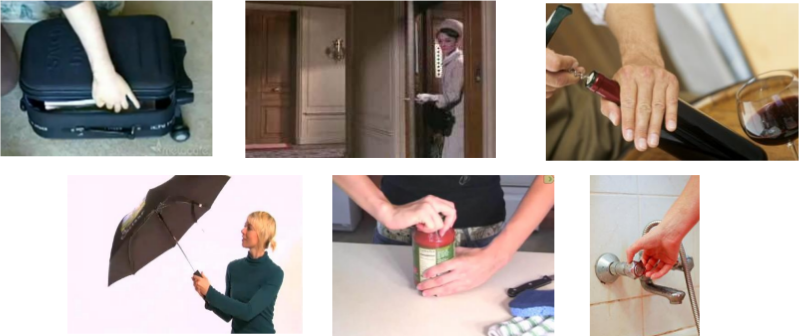
\includegraphics[scale=0.3]{open_example}
  \caption{Examples of ``Open'' action}
  \label{fig:open_example}

\end{figure}

In order to deal with those challenges, several standard action datasets have been created in order to develop
robust human action recognition systems and detection algorithms.
The first datasets included 1 actor performing using a static camera over homogeneous backgrounds.
Even though, those datasets helped us design the first action recognition algorithms, they were not able to deal with the above
challenges.
This lead us to design datasets containing more ambiguous videos, such as Joint-annotated Human Motion Database(JHMDB) (\cite{Kuehne11})
and UCF-101 (\cite{soomro2012ucf101}). These datasets contain only human actions, the second category presented above.

\subsection{JHMDB Dataset}
The JHMDB dataset (\cite{Jhuang:ICCV:2013}) is a fully annotated dataset for human actions and human poses. It is consisted of 21 action categories and 928
clips extracted from Human Motion Database (HMDB51) \cite{Kuehne11}. This dataset contains trimmed videos with duration between
15 to 40 frames. Each clip is annotated for each frame using a 2D pose and contains only 1 action.
In order to train our model for action localization, we modify 2D poses into 2D boxes containing the whole pose in each frame.
There are available 3 different splits for training data, proposed by the authors. We chose the first split which contains 660
videos for training set and 268 for validation . 

\subsection{UCF-101 Dataset}
The UCF-101 dataset (\cite{soomro2012ucf101}) contains 13320 videos from 101 action categories.
From those, for 24 classes and 3194 video spatiotemporal annotations are included. This means that there is a 2D bounding box surrounding the actor for each frame in which an action is taking place.
We separate dataset's videos into 2284 videos for training set and 910 for validation test according to the
first proposed training split. For training data, there are videos up to 641 frames, while in validation data max number of frames is 900.
Each video, both training and validation, is untrimmed, including sometimes more than 1 actions taking place simultaneously.
We took annotations from \cite{singh2016online} because those  proposed by the authors contain some mistakes.

\section{Motivation and Contributions}
The current achievements in Object Recognition Networks and in 3D Convolution Networks for Action Recognition have triggered us to try
to combine them in order to achieve state-of-the-art results for action localization. We introduce a new network structure inspired by
\cite{DBLP:journals/corr/HouCS17}, \cite{DBLP:journals/corr/abs-1712-09184},\cite{Ren:2015:FRT:2969239.2969250} and for implementation
by \cite{jjfaster2rcnn}.

Our contributions are the following:
\begin{enumerate}
\item We create a new framework for action localization extending the code taken from faster RCNN implementation. Based on the structure
  proposed by \cite{DBLP:journals/corr/HouCS17}, we modified it, using a 3D Resnet34 instead of C3D, which previous approach used.

\item Furthermore, we proposed our own TPN Network, a Network for proposing candidate action tubes give a small video segment.
  Following the approach \cite{DBLP:journals/corr/HouCS17} proposed, we firstly implement an architecture which uses
  cuboids as anchors, which then using a regressor it becomes a sequence of bounding boxes, likely to contain an action.
  We experiment with two candidate regressor's architecture and proposed and implement a 3D RoiAlign which uses trilinear
  interpolation for extracting each proposed action tube's activation maps. 
  Inspired by \cite{DBLP:journals/corr/abs-1712-09184}, we proposed and implement a TPN which uses predefined sequences of bounding
  boxes as 3D anchors. We proposed anchors that last equal with and less than video segment's duration in order our architecture to be able to
  perform temporal localization.  we explore two different regressors' architectures for better spatial precision using activation
  maps extracted from 2D RoiAlign, treating each frame separately.
\item Inspired by linking algorithm proposed by \cite{DBLP:journals/corr/HouCS17}, we introduce our own linking algorithm, which
  uses a combination of actioness and overlap scores in order to decide if 2 proposed action tubes would connect or not and some updatable lists.
  Our approach includes gathering all candidate action tubes whose score is bigger than a threshold, and use them as active action tubes for
  new possible connections. When the number of gathered active action tube is bigger than a threshold, we keep the k-best scoring action tubes
  and remove the rest.  We implement this algorithm using, also, CUDA code in order to calculate connection score faster. We proposed 3 versions of this algorithm:
  \begin{enumerate}
  \item An approach which uses an updatable scoring threshold, in order not to calculate unnecessary connection scores
  \item An approach which doesn't use an updatable scoring threshold, but it just updates ``active'' action tube more frequently.
  \item An approach which, also, uses NMS or softmax-NMS algorithms for getting wider action tube proposals.
  \end{enumerate}
  Also, we implement, from scratch, another connection algorithm proposed by \cite{DBLP:journals/corr/abs-1903-00304} and extending it in order to work for ToIs instead of frames, which they proposed.
  We modified our TPN structure in order to calculate progression and progress rate scores in order to calculate connection scores and generate candidate action tubes.
\item We experiment using several classifier in order to find the most suitable. We considered 2 feature maps extracted using 3D RoiAlign and proposed action tubes, without any other
  modification. Also, we explore the different ratios and number of groundtruth foreground tubes that should be used during training
  stage. Finally, we tried to perform only temporal localization using temporal information generated from proposed action tubes.
\end{enumerate}

\section{Thesis structure}
The rest of Thesis is organized as follows. Chapter 2 provides an general introduction to Machine Learning techniques currently used.
After that, we present the basic elements of object recognition systems and alongside with loss functions and evaluation metrics that
we used. Also, Chapter 2 presents an brief overview of literature on human action recognition and localization. Chapter 3 introduces the first basic element of our network, Tube Proposal Network (TPN), a network which proposes Tubes of Interest (ToIs), which are sequences of bounding boxes, with are likely to contain a performed action. Furthermore, it contains all the proposed architectures for achieving this.
Chapter 4 proposes algorithms for linking the proposed TOIs from every video segment and proposal performance is presented.
In Chapter 5, we present all the classification approaches we used for designing our architecture and some classification results.
Chapter 6 is used for conclusions, summary of our contribution alongside with possible future work.

% \end{document}

% \documentclass{report}

% \usepackage{subcaption} % package for subfigures
% \usepackage{hyperref}  % package for linking figures etc
% \usepackage{enumitem}  % package for description with bullets
% \usepackage{graphicx}  % package for importing images
% \usepackage{mathtools} % package for math equation
% \usepackage{mathrsfs}  % package for math font
% \usepackage{indentfirst} % package for getting ident after section or paragraph
% % \usepackage{amsmath}

% \setlength{\parindent}{2em} % how much indent to use when we start a paragraph

% \graphicspath{ {./theory/figures/} }       % path for images

% \begin{document}

\chapter{Background}


\section{Machine Learning}

\subsection{Introduction}
Machine Learning (ML) is a field which is raised out of Artificial Intelligence (AI). Applying AI, we wanted to build better and intelligent
machines. But except for few mere tasks such as finding the shortest path between point A and B, we were unable to program more complex
and constantly evolving challenges. There was a realisation that the only way to be able to achieve this task was to let machine learn
from itself. This sounds similar to a child learning from its self. So machine learning was developed as a new capability for computers.
And now machine learning is present in so many segments of technology, that we don’t even realise it while using it. \par
Finding patterns in data on planet earth is possible only for human brains. The data being very massive, the time taken to compute is
increased, and this is where Machine Learning comes into action, to help people with large data in minimum time. \\
There are three kinds of Machine Learning Algorithms :
 
\begin{enumerate}
\item Supervised Learning
\item Unsupervised Learning
\item Reinforcement Learning
\end{enumerate}

\subsubsection{Supervised Learning}
A majority of practical machine learning uses supervised learning. In supervised learning, the system tries to learn from the previous examples that are given. Speaking mathematically, supervised learning is where you have both input variables (\textit{x}) and output variables (\textit{Y}) and can use an algorithm to derive the mapping function from the input to the output. The mapping function is expressed as
$Y = f(x)$.
\begin{figure}[h]
  \centering
  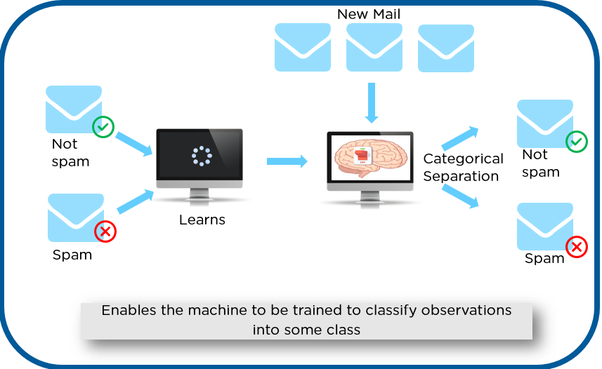
\includegraphics[scale=0.3]{supervised_leaning_example2}
  \caption{Example of supervised Learning}
  \label{fig:supervised_learning_example}
\end{figure}

As shown in Figure \ref{fig:supervised_learning_example}, we have initially taken some data and marked them as ‘Spam’ or ‘Not Spam’. This
labeled data is used by the training supervised model, in order to train the model. Once it is trained, we can test our model by testing it with some test new mails and checking of the model is able to predict the right output. 

Supervised learning problems can be further divided into two parts, namely \textbf{classification}, and \textbf{regression}.
\begin{description}
\item[ Classification] : A classification problem is when the output variable is a category or a group, such as “black” or “white” or “spam” and “no spam”.
\item[ Regression ] :  A regression problem is when the output variable is a real value, such as “Rupees” or “height.”
\end{description}
Some Supervised learning algorithms include:
\begin{itemize}
\item Decision trees
\item Support-vector machine
\item Naive Bayes classifier
\item k-nearest neighbors
\item linear regression
\end{itemize}

\subsubsection{Unsupervised Learning}

In unsupervised learning, the algorithms are left to themselves to discover interesting structures in the data. Mathematically, unsupervised
learning is when you only have input data (\textit{X}) and no corresponding output variables. This is called unsupervised learning because
unlike supervised learning above, there are no given correct answers and the machine itself finds the answers.
\begin{figure}[h]
  \centering
  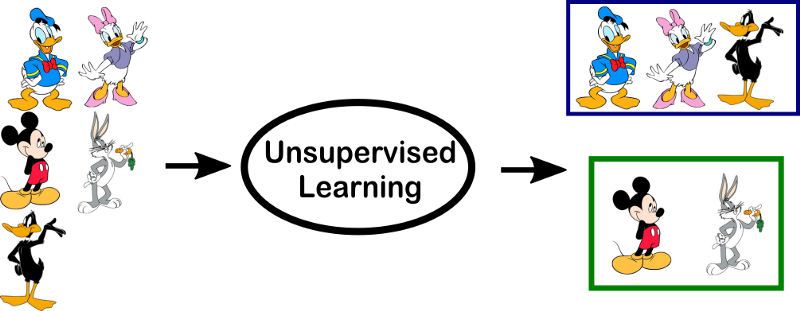
\includegraphics[scale=0.3]{unsupervised_learning_example}
  \caption{Example of unsupervised Learning}
  \label{fig:unsupervised_learning_example}
\end{figure}
In Figure \ref{fig:unsupervised_learning_example}, we have given some characters to our model which are ‘Ducks’ and ‘Not Ducks’. In our
training data, we don’t provide any label to the corresponding data. The unsupervised model is able to separate both the characters by
looking at the type of data and models the underlying structure or distribution in the data in order to learn more about it. Unsupervised
learning problems can be further divided into \textbf{association} and \textbf{clustering} problems.

\begin{description}
\item[ Association] : An association rule learning problem is where you want to discover rules that describe large portions of your data, such as “people that buy X also tend to buy Y”.
\item[ Clustering] : A clustering problem is where you want to discover the inherent groupings in the data, such as grouping customers by purchasing behaviour.
\end{description}

\subsubsection{Reinforcement Learning}
A computer program will interact with a dynamic environment in which it must perform a particular goal (such as playing a game with an
opponent or driving a car). The program is provided feedback in terms of rewards and punishments as it navigates its problem space. 
Using this algorithm, the machine is trained to make specific decisions. It works this way: the machine is exposed to an environment
where it continuously trains itself using trial and error method.
\begin{figure}[h]
  \centering
  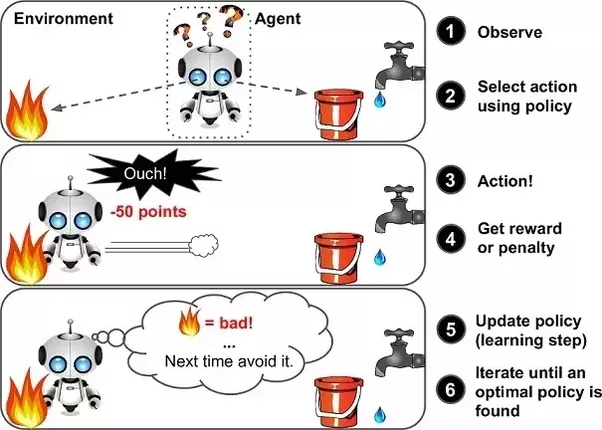
\includegraphics[scale=0.3]{reinforment_learning_example}
  \caption{Example of Reinforcement Learning}
  \label{fig:reinforment_learning_example}
\end{figure}
In Figure \ref{fig:reinforment_learning_example}, we can see that the agent is given 2 options i.e. a path with water or a path with fire. A reinforcement algorithm
works on reward a system i.e. if the agent uses the fire path then the rewards are subtracted and agent tries to learn that it should avoid
the fire path. If it had chosen the water path or the safe path then some points would have been added to the reward points, the agent then
would try to learn what path is safe and what path isn’t

\subsection{Neural Networks}
Neural Networks are a class of models within the general machine learning literature. Neural networks are a specific set of algorithms that
have revolutionized the field of machine learning. They are inspired by biological neural networks and the current so called deep neural
networks have proven to work quite very well. Neural Networks are themselves general function approximations, that is why they can be applied
to literally almost any machine learning problem where the problem is about learning a complex mapping from the input to the output space.

\subsection{A single Neuron}
The basic unit of computation in a neural network is the neuron, often called a \textbf{node} or \textbf{unit}. It receives input from some
other nodes, or from an external source and computes an output. In purely mathematical terms, a neuron in the machine learning world is a
placeholder for a mathematical function, and its only job is to provide an output by applying the function on the inputs provided.
Each input has an associated weight (\textit{w}), which is assigned on the basis of its relative importance to other inputs. The node applies
a function \textit{f  (defined below)} to the weighted sum of its inputs as shown in Figure \ref{fig:Perceptron}.
\begin{figure}[h]
  \centering
  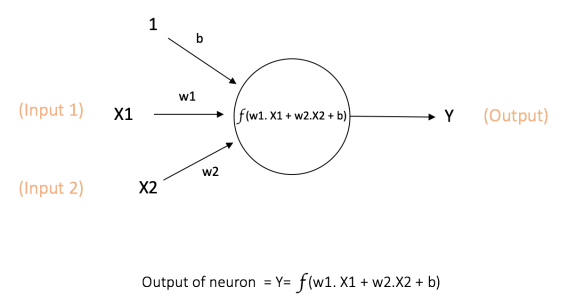
\includegraphics[scale=1.0]{perceptron}
  \caption{An example of a single Neuron}
  \label{fig:Perceptron}
\end{figure}
The network takes numerical inputs \textit{X1} and \textit{X2} and has weights \textit{w1} and \textit{w2} associated with those inputs.
Additionally, there is another \textit{input 1} with weight \textit{b} (called \textit{Bias}) associated with it. The main function of Bias is to provide every node with a trainable constant value (in addition to the normal inputs that the node receives). The output Y from the neuron
is computed as shown in the Figure \ref{fig:Perceptron}. The function \textit{f} is non-linear and is called \textbf{Activation Function}. The
purpose of the activation function is to introduce non-linearity into the output of a neuron. This is important because most real world data
are non linear and we want neurons to learn these non-linear representations.
\subsubsection{Activation Functions} 
Every activation function (or non-linearity) takes a single number and performs a certain fixed mathematical operation on it. There are
several activation functions:
\begin{description}
\item[ Sigmoid ] : takes a real-valued input and squashes it to range between 0 and 1. Its formula is:
  \[ \sigma(x) = \frac{1}{1 + e^{-x} } \]
  It is easy to understand and apply but it has major reasons which have made it fall out of popularity:
  \begin{itemize}
  \item Vanishing gradient problem
  \item Its output isn’t zero centered. It makes the gradient updates go too far in different directions.
  \item Sigmoids saturate and kill gradients.
  \item Sigmoids have slow convergence.
  \end{itemize}

\item [ Tanh ] : takes a real-valued input and squashes it to the range [-1, 1]. Its formula is:
  \[ tanh(x) = 2 \sigma(2x) -1 \]
  Now it’s output is zero centered because its range in between -1 to 1. Hence optimization is easier in this method and  in practice it is always preferred over Sigmoid function . But still it suffers from Vanishing gradient problem.

\item[ ReLU ]: ReLU stands for \textit{Rectified Linear Unit}. It takes a real-valued input and thresholds it at zero (replaces negative values with zero). So its formula is:
  \[ f(x) = max(0,x) \]
  It has become very popular in the past couple of years. It was recently proved that it had 6 times improvement in convergence from Tanh
  function. Seeing the mathamatical form of this function we can see that it is very simple and efficinent . A lot of times in Machine
  learning and computer science we notice that most simple and consistent techniques and methods are only preferred and are best.
  Hence it avoids and rectifies vanishing gradient problem . Almost all deep learning Models use ReLu nowadays.
\end{description}

Figure \ref{fig:Activation}  show each of the above activation functions.
\begin{figure}[h]
  \centering
  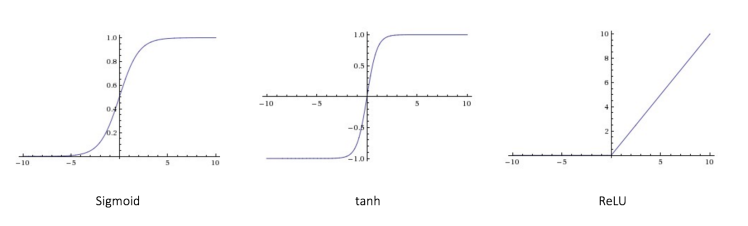
\includegraphics[scale=1.0]{activation_figures}
  \caption{Plots of Activation functions}
  \label{fig:Activation}
\end{figure}

\subsubsection{Feedforward Neural Network}
Till now we have covered neuron and activation functions which together for the basic building blocks of any neural network. The feedforward
neural network was the first and simplest type of artificial neural network devised. It contains multiple neurons (nodes) arranged in layers.
A layer is nothing but a collection of neurons which take in an input and provide an output. Inputs to each of these neurons are processed
through the activation functions assigned to the neurons. Nodes from adjacent layers have connections or edges between them. All these connections have weights associated with them.
\begin{figure}[h]
  \centering
  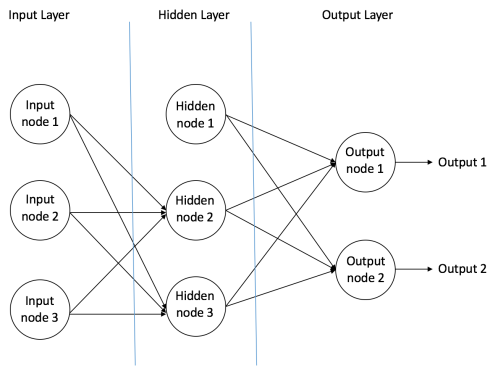
\includegraphics[scale=1.0]{feedforwardnetwork}
  \caption{An example of a Feedforward Neural Network}
  \label{fig:feedforwardnetwork}
\end{figure}
An example of a feedforward neural network is shown in Figure \ref{fig:feedforwardnetwork}. A feedforward neural network can consist of three types of nodes:
\begin{description}
\item[ Input Nodes ] The Input nodes provide information from the outside world to the network and are together referred to as the
  “Input Layer”. No computation is performed in any of the Input nodes – they just pass on the information to the hidden nodes.
\item[  Hidden Nodes ]  The Hidden nodes have no direct connection with the outside world (hence the name “hidden”). They perform
  computations and transfer information from the input nodes to the output nodes. A collection of hidden nodes forms a “Hidden Layer”.
  While a feedforward network will only have a single input layer and a single output layer, it can have zero or multiple Hidden Layers.
\item [ Output Nodes ] The Output nodes are collectively referred to as the “Output Layer” and are responsible for computations and
  transferring information from the network to the outside world.
\end{description}

In a feedforward network, the information moves in only one direction – forward – from the input nodes, through the hidden nodes (if any)
and to the output nodes. There are no cycles or loops in the network (this property of feed forward networks is different from Recurrent
Neural Networks in which the connections between the nodes form a cycle). Another important point to note here is that each of the hidden
layers can have a different activation function, for instance, hidden layer1 may use a sigmoid function and hidden layer2 may use a ReLU,
followed by a Tanh in hidden layer3 all in the same neural network. Choice of the activation function to be used again depends on the
problem in question and the type of data being used.

\subsection {2D Convolutional Neural Network}
A Convolutional Neural Network (ConvNet/CNN) is one of the variants of neural networks used heavily in the field of Computer Vision. It
derives its name from the type of hidden layers it consists of. The hidden layers of a CNN typically consist of convolutional layers, pooling
layers, fully connected layers, and normalization layers. Here it simply means that instead of using the normal activation functions defined
above, convolution and pooling functions are used as activation functions.
It can take in an input image, assing importance (learning weights and biases) to various aspects/objects in the image and be able to
differentiate one from the other. The pre-processing required in a ConvNet is much lower as compared to the other classification algorithms.
While in primitive method filters are hand-engineered, with enough training, ConvNets have the ability to learn these filters/characteristics.

The architecture of a ConvNet is analogous to that of the connectivity pattern of Neurons in the Human Brain and was inspired by the
structure of the Visual Cortex. However, most ConvNets costist mainly in 2 parts:
\begin{description}[font=$\bullet$\scshape\bfseries]
\item [ Feature extractor] : \\
  This part of the network takes as input the image and extract features that are meaningful for its classification. It amplifies aspects
  of the input that are important for discrimination and suppresses irrelevant variations. Usually, the feature extractor cosists of
  several layers. For instance, an image which could be seen as an array of pixel values. The first layer often learns reprensations
  that represent the presence or absence of edges at particular orientations and locations in the image. The second layer typically
  detects motifs by spotting particular arrangements of edges, regardeless of small variations in the edge positions. Finally, the third
  may assemble motifs into larger combinations that correspond to paths of familiar objects, and subsequent layers would detect objects
  as combinations of these parts.
  
\item [ Classifier ] : \\
  This part of the network takes as input the previously computed features and use them to predict the correct label.
\end{description}

\begin{figure}[h]
  % 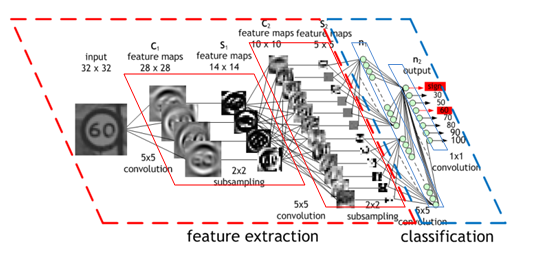
\includegraphics[scale=0.7]{convolutional_neural_network_structure} \]
  \centering
  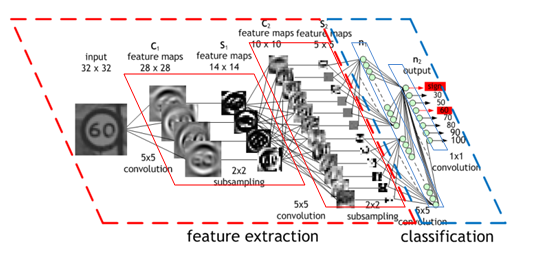
\includegraphics[scale=0.7]{convolutional_neural_network_structure}
  \caption{Typical structure of a ConvNet}
\end{figure}
\paragraph{Convolutional Layers}
In order to extract such features, ConvNets use 2D convolution operations. These operations take place in convolutional layers. Convolutional
layers consist of a set of learnable filters. Every filter is small spatially (along widht and height), but extends through the full depth of
input. During forword pass, we slide (more precisely, convolve) each filter across the width and height of the input volume and compute dot
products between the entries of the filter and the input at any position (as Figure \ref{fig:conv_example} shows). The objective of the
Convolution Operation is to extract the high-level features such as edges, from the input image. ConvNets need not be limited to only one
Convolutional Layer. Conventionally, the first ConvLayer is responsible for capturing the Low-Level features such as edges, color, gradient
orientation, etc. With added layers, the architecture adapts to the High-Level features as well, giving us a network which has the wholesome
understanding of images in the dataset, similar to how we would.

\begin{figure}[h]
  \centering
  \begin{minipage}[b]{0.4\textwidth}
    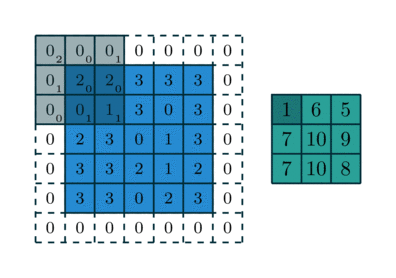
\includegraphics[width=\textwidth]{conv_1}
  \end{minipage}
  \hfill
  \begin{minipage}[b]{0.4\textwidth}
    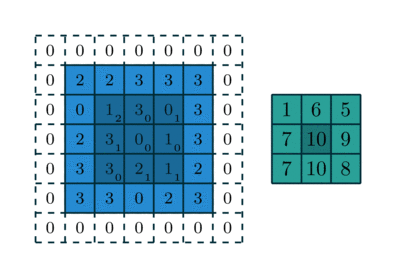
\includegraphics[width=\textwidth]{conv_2}
  \end{minipage}
  \caption{Convolution with kernel of 3, stride of 2 and padding of 1}
  \label{fig:conv_example}
\end{figure}
\paragraph{Pooling Layers}
Pooling Layers are also refered as downsampling layers and are used to reduce the spatial dimensions, but not depth, on a convolution neural network.
The intuitive reasoning behind this layer is that once we know that a specific feature is in the original input volume (there will be a high activation value),
its exact location is not as important as its relative location to the other features. The main advantages of pooling layer are:

\begin{itemize}
\item We gain computation performance since the amount of parameters is reduce.
\item Less parameters also means We deal with overfitting situations.
\end{itemize}

The pooling operation is specified, rather than learned. Two common functions used in the pooling operation are:
\begin{description}
\item[ Average Pooling ] Calculate the average value for each patch on the feature map.
\item[ Maximum Pooling (or Max Pooling) ] Calculate the maximum value for each patch of the feature map.
\end{description}

\begin{figure}[h]
  \centering
  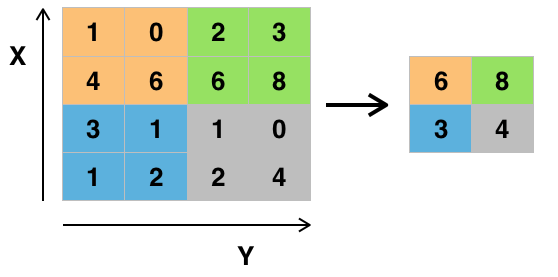
\includegraphics[scale=0.35]{max_pooling}
  \caption{Example of Max pooling operation with a 2x2 filter  and stride of 2}
  \label{fig:pooling_eg}
\end{figure}

\subsection{3D Convolutional Neural Network}
Traditionally, ConvNets are targeting RGB images (3 channels). The goal of 3D CNN is to take as input a video and extract features from it.
When ConvNets extract the graphical characteristics of a single image and put them in a vector (a low-level representation), 3D ConvNets
extract the graphical characteristics of a set of images. 3D CNNs takes in to account a temporal dimension (the order of the images in the
video). From a set of images, 3D CNNs find a low-level representation of a set of images, and this representation is useful to find the
right label of the video (a given action is performed). \\
In order to extract such features, 3D ConvNets  use 3D convolution operations.
\begin{figure}[h]
  % 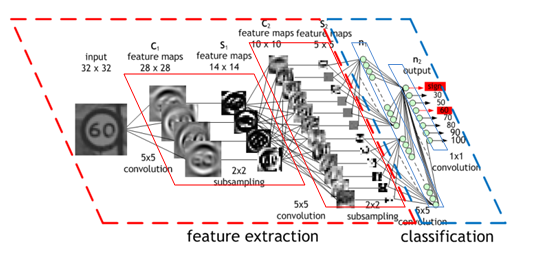
\includegraphics[scale=0.7]{convolutional_neural_network_structure} \]
  \centering
  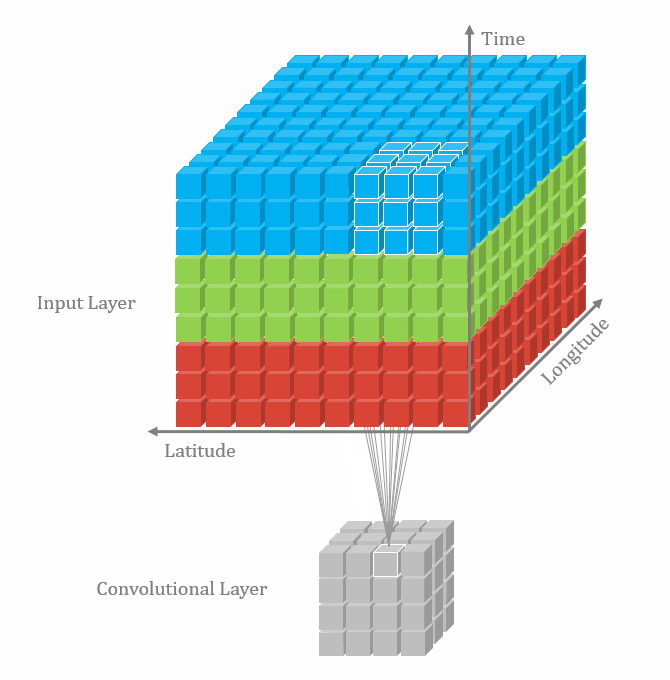
\includegraphics[scale=0.3]{3d_conv}
  \caption{3D Convolution operation}
\end{figure}

There are several existing approaches to tackle the video classification. This is a nonexaustive list of existing approaches:
\begin{description} [font=$\bullet$\scshape\bfseries]
\item[ ConvNets + LSTM cell] : Extract features from each frame with a ConvNet, passing the sequence to an RNN
\item[ Temporal Relation Networks] : Extract features from each frame with a ConvNet and pass the sequence to an MLP
\item[ Two-Stream Convolutional Networks] : Use 2 CNN, 1 spatial stream ConvNet which process one single frame at a time, and 1 Temporal stream ConvNet which process multi-frame optical flow
\end{description}

\section{Object Detection}
Within the field of Deep Learning, the sub-discipline called “Object Detection” involves processes such as identifying the objects through a picture, video or a webcam feed.
Object Detection is used almost everywhere these days. The use cases are endless such as Tracking objects, Video surveillance, Pedestrian detection etc. 
An object detection model is trained to detect the presence and location of multiple classes of objects. For example, a model might be trained with images that
contain various pieces of fruit, along with a label that specifies the class of fruit they represent (e.g. an apple, a banana, or a strawberry),
and data specifying where each object appears in the image.

The main process followed by most of CNN for Object Detection is:
\begin{enumerate}
\item Fistly, we do feature extraction using as backbone network, the first Convolutional Layers of a known pre-trained CNN such
  as AlexNet, VGG, ResNet etc.
\item Then, we propose regions of interest (ROI) in the image. These regions contain possibly an object, which we are looking for.
\item Finally, we classify each proposed ROI.
\end{enumerate}

\subsection{ Region Proposal Network}

From the 3 above steps, the 2nd step is considered to be very important. That is because, in this step, we should choose regions of
the image, which will be classified. Poor choice of ROIs means that the CNN will pass by some object that are located in the image,
because, they were not be proposed to be classified.

\begin{figure}[h]
  \centering
  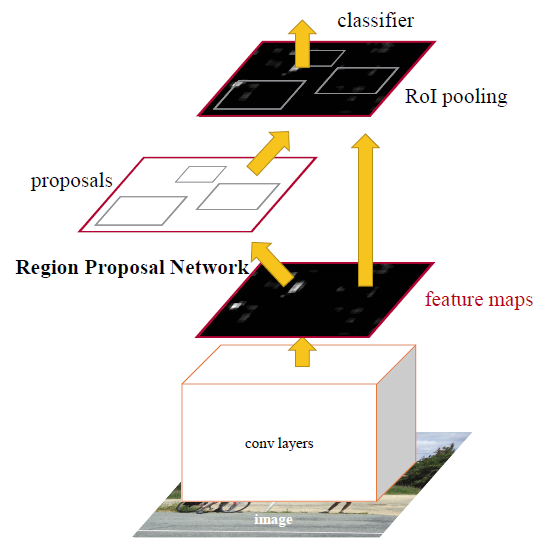
\includegraphics[scale=0.3]{RPN_structure}
  \caption{ Region Proposal Network's structure}
  \label{fig:rpn_structure}
\end{figure}

The first Object-Detection CNNs use several algorithms for proposing ROIs. For example, R-CNN\cite{DBLP:journals/corr/GirshickDDM13},
and Fast R-CNN\cite{Girshick:2015:FR:2919332.2920125} used Selective Search Algorithm for extracting ROIs.
One of noverlties introduced by the Faster R-CNN\cite{Ren:2015:FRT:2969239.2969250} is \textbf{Region Proposal Network} (RPN). Its
Function is to propose ROIs and its structure can be shown in \ref{fig:rpn_structure}. As we can see, RPN is consisted of:
\begin{itemize}
\item 1 2D Convolutional Layer
\item 1 score layer 
\item 1 regression layer
\end{itemize}

Another basic element of RPN is the \textbf{anchors}. Anchors are predefined boxes used for extracting ROIs. In figure \ref{fig:anchors} is
depicted an exaple of some anchors
\begin{figure}[h]
  \centering
  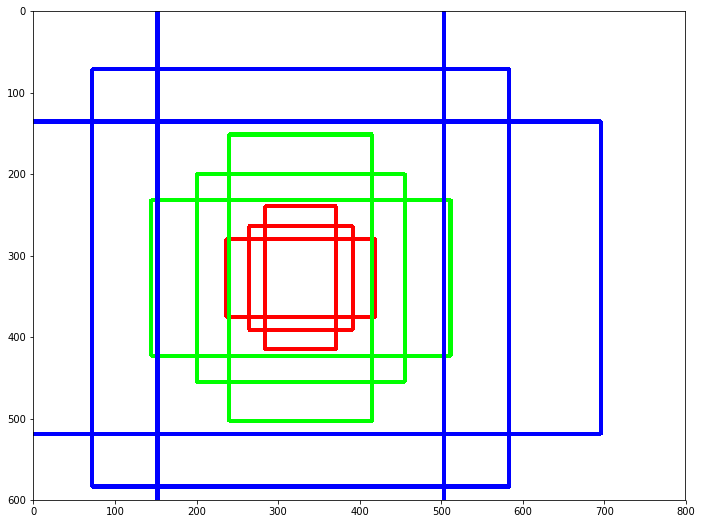
\includegraphics[scale=0.3]{anchors}
  \caption{ Anchors for pixel (320,320) of an image (600,800) }
  \label{fig:anchors}
\end{figure}

For each feature map's pixel corresponds \textbf{k (k=9)} anchors (3 different scales and 3 different ratios 1:1, 1:2, 2:1). \par
As a result, RPN gets as input feature maps extracted from the backbone CNN. Then performs 2D convolution over this input and passes
the output to its scoring layer and regression layer. Those scores represent the confidence of existing an object in this specific position.
On top of that, regression layer outputs 4k displacements, 4 for each anchor. Finally, we keep as output only the \textit{ n-best scoring} anchors.

\subsection{Roi Align}

\subsection{Non-maximum suppression (NMS) algorithm}

\section{Losses and Metrics}
In order to train our model and check its performance, we use some known Loss functions and Metrics used in Object Detection systems.
\subsection{Losses}
For training our network, we use \textbf{Cross Entropy Loss} for classification layers and \textbf{smooth L1-loss} for bounding box regression
in each frame and their diagram is show at Figure \ref{fig:cross_l1}.
\subsubsection{Cross Entropy Loss}
Cross-entropy loss, or log loss, measures the performance of a classification model whose output is a probability value between 0 and 1. \par
Entropy is the measure of uncertainty assosiated with a given distribution \textit{q(y)} and its formula is: 
\[ H = -\sum_{i=1}^n p_i \cdot \log p_i \]
Intuitively, entropy tells us how ``surprised'' we are when some event E happened. When we are sure about an event E to happened ($ p_E = 1$)
we have 0 entropy (we are not surprised) and vise versa. \par
On top of that, let's assume that we have 2 distributions, one known (our network's distribution) \textit{p(y)} and one unknown (the actual
data's distribution) \textit{q(y)}. Cross-entropy tells us how accurate is our known distribution in predicting the unknown distribution's
results. Respectively, Cross-entropy measures how accurate is our model in predicting the test data. Its formula is:
\[ H_p(q) = - \sum_{c=1}^C q(y_c) \cdot log(p(y_c)) \]

\subsubsection{Smooth L1-loss}

Smooth L1-loss can be interpreted as a combination of L1-loss and L2-loss. It behaves as L1-loss when the absolute
value of the argument is high, and it behaves like L2-loss when the absolute value of the argument is close to zero.
It is usually used for doing box regression on some object detection systems like Fast-RCNN(\cite{Girshick:2015:FR:2919332.2920125}),
Faster-RCNN(\cite{Ren:2015:FRT:2969239.2969250}) and it is less sensitive to outliers according according to \cite{Girshick:2015:FR:2919332.2920125}.
As showm in \cite{Girshick:2015:FR:2919332.2920125}, its formula is:

\[ smooth_{L1}(x) = \begin{dcases}
    0.5x^2 & \text{ if } x < 1 \\
    |x| - 0.5 & \text{otherwise}
  \end{dcases}\]

It is similar to Huber loss whose formula is:

\[
L_{\delta}(x) = \begin{dcases}
    \frac{1}{2}a^2 & \text{ for } |a| \le \delta \\
\delta(|a| - \frac{1}{2}\delta), & \text{otherwise}
\end{dcases}
\]

if we set $\delta $ parameter equal 1. \par

Smooth L1-loss combines the advantages of L1-loss (steady gradients for large values of \textit{x}) and L2-loss (less oscillations during
updates when \textit{x} is small). Figure \ref{fig:cross_l1} \subref{fig:smooth_l1} shows a comparison between L1-norm, L2-norm  and smooth-L1 .

\begin{figure}[h]
  \centering
  \begin{subfigure}{0.45\textwidth}
    % \fbox{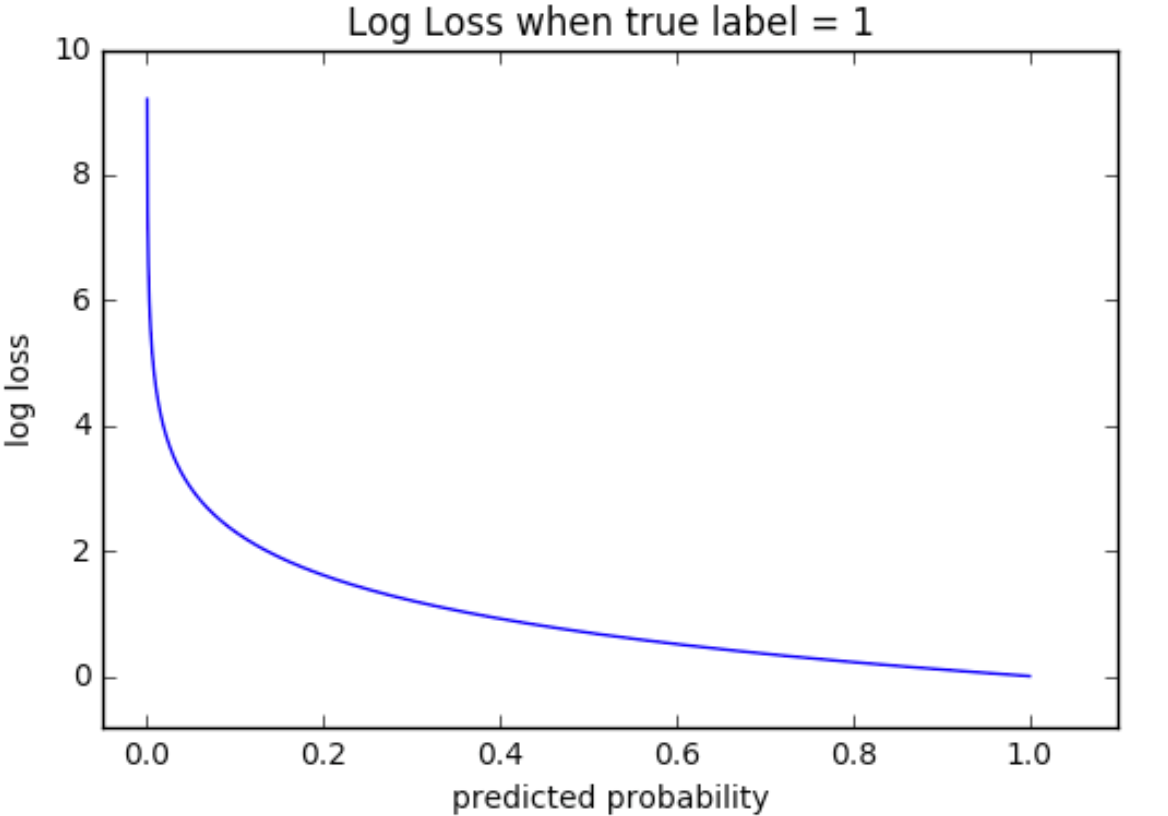
\includegraphics[width=\textwidth]{c_entropy}}
    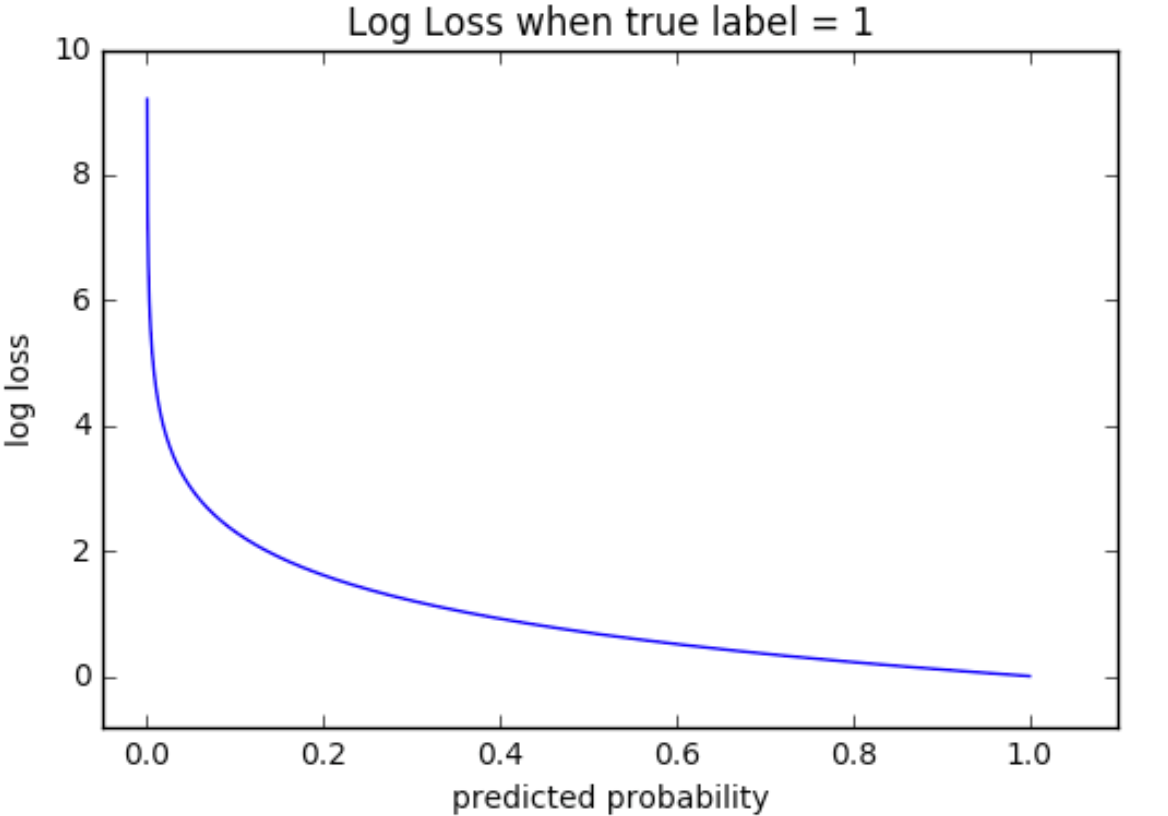
\includegraphics[width=\textwidth]{c_entropy}

      \caption{}
      \label{fig:cross_entropy}

  \end{subfigure}
  \hfill
  \begin{subfigure}{0.51\textwidth}
% \fbox{    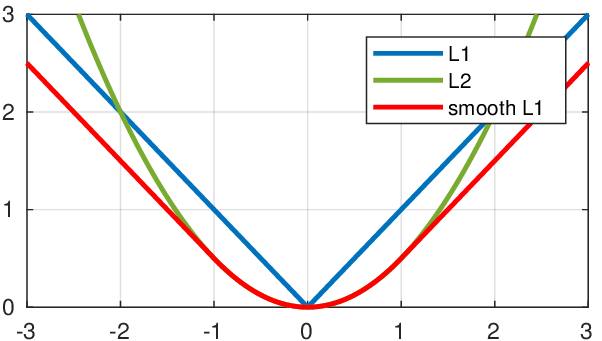
\includegraphics [width=5.5cm,height=3.8cm]{smooth_l1}}
    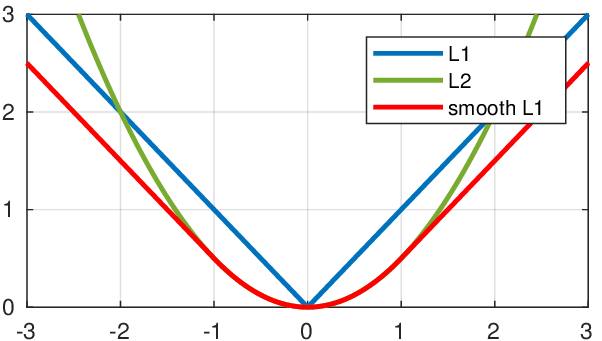
\includegraphics [width=5.5cm,height=3.8cm]{smooth_l1}
    % 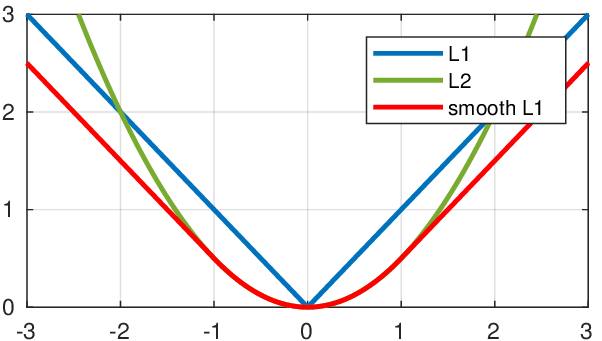
\includegraphics[width=\textwidth]{smooth_l1}
      \caption{}
      \label{fig:smooth_l1}
  \end{subfigure}

  \caption{ (\subref{fig:cross_entropy}) and (\subref{fig:smooth_l1})  show the behavior of cross-entropy loss and smooth-L1 respectively.}
  \label{fig:cross_l1}%
\end{figure}

\subsection{Metrics}
Evaluating our machine learning algorithm is an essential part of any project. The way we choose our metrics influences how the performance
of machine learning algorithms is measured and compared.
They influence how to weight the importance of different characteristics in the results and finally,
the ultimate choice of which algorithm to choose. Most of the times we use classification accuracy
to measure the performance of our model, however it is not enough to truly judge our model. \par
At first, we introduce some basic evaluation metrics in order,then, to present those we use for our assesment.

\subsection{Intersection over Union}
The first and most important metric that we use is Intersection over Union (IoU). IoU  measures the overlap between 2 boundaries.
It is usually used in Object Recognition Networks in order to define how good overlap a predicted bounding box  with the actuall
bounding box as shown in Figure \ref{fig:iou_fig}. We predefine an IoU threshold (say 0.5) in classifying whether the prediction is a true positive or a false positive.
\begin{figure}[h]
  \centering
  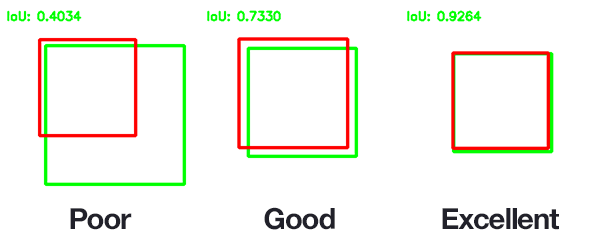
\includegraphics[scale=0.55]{iou}
  \caption{Example of IoU scoring policy}
  \label{fig:iou_fig}
\end{figure}

Intersection over Union is defined as:
\[ IoU = \frac{\text{area of overlap}}{\text{area of union}} \]
In Figure \ref{fig:iou_fig}, spatial IoU between 2 bounding boxes, $(x_1,y_1,x_2,y_2)$ and $(x_3,y_3,x_4,y_4)$,is presented, which means IoU metric is implemented for x-y dimensions.
Area of overlap and area of union can be defined as:
\[\text{ Area of overlap } = \lVert( min(x_2,x_4) - max(x_1,x_3), min(y_2,y_4)- max(y_1,y_3) )\rVert\]
\[\text{ Area of union  }  = \lVert( max(x_2,x_4) - min(x_1,x_3), max(y_2,y_4) - min(y_1,y_3) )\rVert\]
On top of that, we can implement IoU for 1 dimension and for 3 dimensions.
\paragraph{1D IoU} We can name 1D IoU as temporal overlap. Let's consider 2 temporal segments $(t_1,t_2)$ and $(t_3,t_4)$, between which we want to
estimate their overlap score. Their IoU can be described as:
\[ \text { Length of overlap } = \lVert(min(t_2,t_4) - max(t_1,t_3))\rVert  \]
\[ \text { Length of union } = \lVert(max(t_2,t_4) - min(t_1,t_3))\rVert  \]
\paragraph{3D IoU} 3-dimentional Intersection over Union which can, also, be named as spatiotemporal IoU, can be defined by 2 ways:
% categories: whether the $3^{rd}$ dimension is continuous or discrete.
\begin{description}
\item[3D boxes are cuboids] In this case, 3D boxes can be written  as $(x,y,z,x',y',z')$. So, the IoU overlap between 2 boxes, $(x_1,y_1,z_1,x_2,y_2,z_2)$
  and $(x_3,y_3,z_3,x_4,y_4,z_4)$, is defined as:
\[ \text { Volume of overlap } = \lVert(min(x_2,x_4) - max(x_1,x_3),min(y_2,y_4) -  max(y_1,y_3), min(z_2,z_4) -  max(z_1,z_3) ) \rVert \]
\[ \text { Volume of union } = \lVert(max(x_2,x_4) - min(x_1,x_3), max(y_2,y_4) - min(y_1,y_3), max(z_2,z_4) - min(z_1,z_3)  \]

\item[x-y are continuous and z discrete] In this case 3D boxes is defined as a sequence of 2D boxes $(x,y,x',y')$. For this definition, z-dimension is
  discrete, and IoU can be defined with 2 ways, which both result in the same overlapping score. Let's cosider 2 sequences of boxes, with temporal limits
  $(t_1,t_2)$ and $(t_3,t_4)$. We calculate their IoU following one of the following methods:
  \begin{enumerate}
\item IoU is the product between temporal-IoU and the average spatial-IoU between 2D boxes in the overlapping temporal area and it is described as:
\[ IoU =  IoU((t_1,t_2),(t_3,t_4)) \cdot \frac{1}{K_2-K_1} \sum_{i=K_1}^{K_2} IoU(X_1^i, X_2^i) \]
  where \begin{itemize}
  \item$K_1 = min(t_2,t_4)$
  \item$K_2 = max(t_1,t_3)$
  \item$ X_1^i =  (x_1^i,y_1^i,x_2^i,y_2^i)$ and $X_2^i =  (x_3^i,y_3^i,x_4^i,y_4^i) $
  \end{itemize}
\item IoU is the average spatial-IoU if we consider 2D boxes as $(0,0,0,0)$ if $ t \notin [t_{start},t_{finish}]$ and it is written as:
  \[ IoU = \frac{1}{K} \sum_{i = min(t_1,t_3}^{max(t_2,t_4)} IoU(X_1^i,X_2^i) \]
  \begin{itemize}
  \item $K = max(t_2,t_4) - min(t_1,t_3)$
  \item $ X_1 = (x_1,y_1,x_2,y_2)  \text{ if } i \in [t_1,t_2] \text{ or }
        (0,0,0,0)  \text{ if } i \notin [t_1,t_2]  $
  \item $ X_2 = (x_3,y_3,x_4,y_4)  \text{ if } i \in [t_3,t_4] \text{ or }
        (0,0,0,0)  \text{ if } i \notin [t_3,t_4]  $
    \end{itemize}
  
\end{enumerate}
\end{description}
From above implementations, we are involve mostly with temporal and spatiotemporal IoU.

\subsection{Precision  \& Recall }

In order to describe \textbf{precision} and \textbf{recall} metrics, we will use an example. Let's consider a group of people in which, some of them are sick and
the others are not. We use a network which is able to predict if a person is sick or not if we give it some data as input.
\begin{description}
\item[ Precision ]  measures how accurate are our model's predictions. i.e. the percentage of  predictions that are correct.
  In our case, how accurate is our model when it predicts that a person is sick.
\item[ Recall ] measures how good we found all the sick people. In our case, how many of the acctual sick people we managed to find.
\end{description}
Their definisions are:
\[ Precision = \frac{TP}{TP + FP} \]  
\[  Recall = \frac{TP}{TP + FN} \] 
where \begin{itemize}
\item TP = True positive, which means that we predict a person to be sick and he is actually sick.
\item TN = True negative, we predict that a person isn't sick and he isn't.
\item FP = False positive, we predict a person to be sick but he isn't actually.
\item FN = False negative, we predict a person not to be sick but he actually is.
\end{itemize}

From these 2 metrics we use recall metric in order to evaluate our networks performance, and more specifically, its performance on finding good action tube proposals.
We consider a groundtruth action as true positive when there is at least 1 proposed action tube that its IoU overlap score is bigger that
a predifed threshold. If there is no such action tube, then we consider this groundtruth action tube as false negative.


\subsection{mAP - TODO}
Precision and recall are single-value metrics based on the whole list of predictions. By looking their formulas, we can see that there is
a trade-off between precision and recall performance. This trade-off can be adjusted by the softmax threshold, used in model's final layer.
In order to have high precision performance, we need to decrease the number of FP. But this will lead to decrease recall performance and
vice-versa. \par
As a result, these metrics fail to determine if a model is performing well in object detection tasks as well as action detection tasks. For
that reason, we use mAP metric
\paragraph{AP (Average precision)} is a popular metric in measuring the accuracy of object detectors like Faster R-CNN, SSD, etc. Average precision computes the average precision value for recall value over 0 to 1.

In our case, we use the metrics presented in \cite{DBLP:journals/corr/GkioxariM14} in
order to quantify our results:
\begin{description}
% \item[ frame-AP ] measures the area under the precision-recallcurve of the detections for each frame (similar to the PASCAL  VOC  detection  challenge  \cite{Everingham10}).   A  detection is correct
%   if the intersection-over-union with theground truth at that frame is greater than and the ac-tion label is correctly predicted.
\item [ video-AP ] measures the area under the precision-recallcurve of the action tubes predictions. A tube is correctif the mean per frame intersection-over-union with theground truth across the
  frames of the video is greaterthan and the action label is correctly predicted.
% \item [ AUC ] measures the area under the ROC curve, a metricpreviously used on this task.  An action tube is correctunder the same conditions as invideo-AP. Following
%   \cite{Tian:2013:SDP:2514950.2515975} , the ROC curve is plotted until a false positive rateof 0.6, while keeping the top-3 detections per class andper video. Consequently,
%   the best possible AUC scoreis 60\%.
\end{description}

\subsection{MABO}

In order to evaluate more the quality of our proposals, both during TPN and connecting tube stages, recall metric isn't enough. That's because recall metric tells us only in how many
known objects there was at least 1 proposal that satified the detection criterion. However, it doen't tells us how much good. This can be better clarify if we consider figure \ref{fig:mabo_fig}.

\begin{figure}[h]
  \centering
  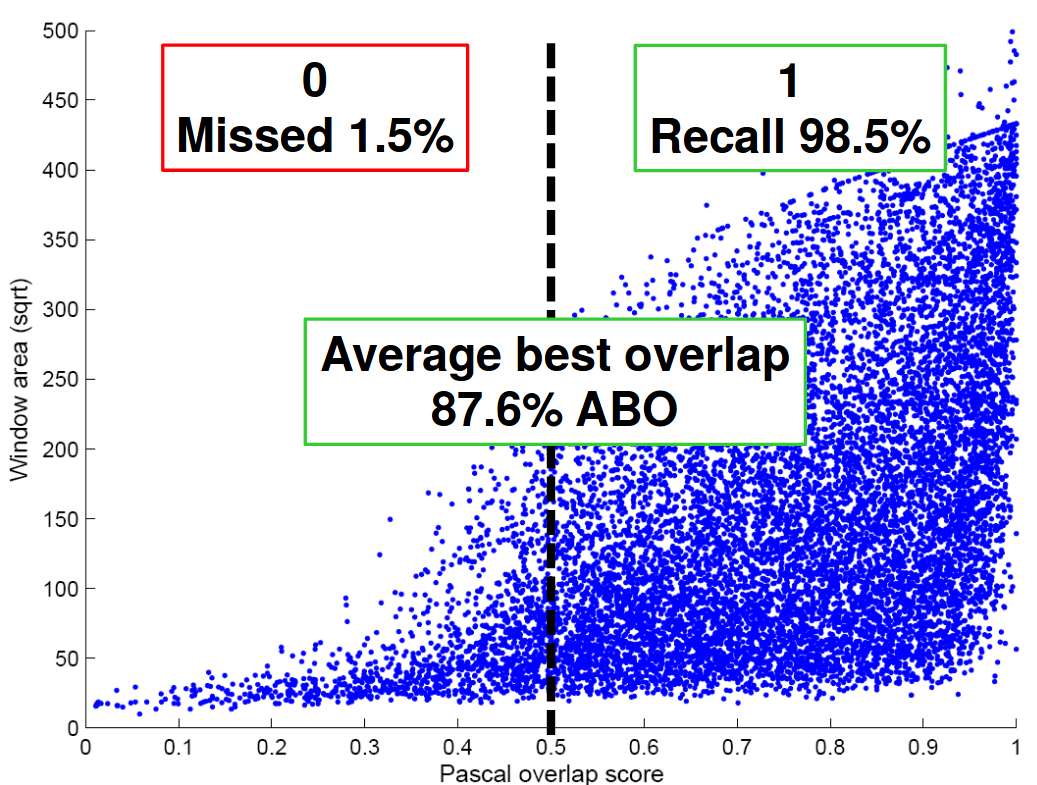
\includegraphics[scale=0.25]{mabo}
  \caption{Example of Max pooling operation with a 2x2 filter  and stride of 2}
  \label{fig:mabo_fig}
\end{figure}


% \end{document}
% \documentclass{report}

% \usepackage{hyperref}  % package for linking figures etc
% \usepackage{enumitem}  % package for description with bullets
% \usepackage{graphicx}  % package for importing images
% \usepackage{mathtools} % package for math equation
% \usepackage{mathrsfs}  % package for math font
% \usepackage{indentfirst} % package for getting ident after section or paragraph
% % \usepackage{amsmath}
% \usepackage[
%     backend=bibtex,
%     citestyle=authoryear,
%     % citestyle=authoryear-comp,
%     % citestyle=authoryear-ibid,
%     bibstyle=numeric,
%     sorting=ynt,
%     % style=numeric,
%     % style=alphabetic ,
%   ]{biblatex}
 
%  \addbibresource{References}
% \setlength{\parindent}{2em} % how much indent to use when we start a paragraph

% \graphicspath{ {./theory/figures/} }       % path for images

% \begin{document}

\chapter{Related work}


% The combination of CNN and Recurrent Neural Network (RNN) is a method widely been studied and achieved excellent results.
% The recently proposed methods can be seperated into 2 subcategories: (1) use a CNN detector in order to localize directly
% the action instance for each single frame and (2) modify the detector in order to get as input volute multiple frames and
% use 3D convolution.%  Both approaches produce the same type of output : i) an actioness score of a bounding box or a proposed
% tube ii) coordinate offsets for bounding box refinement and iii) clasification probabilities for all action classes.

% The task of action classification in approaches used features based on shape or motion sucha as HOG \cite{dalal2005histogramcvpr},
% SIFT \cite{Lowe2004}, MBH \cite{dalal2006human} and train a classifier as SVM.

% \paragraph{Frame based methods}
\section{Action Recognition}
First approaches for action classification consisted of two steps a) compute complex handcrafted features from raw video frames
such as SIFT, HOG, ORB features and b) train a classifier based on those features. These approaches made the choise of
features a signifact factor for network's performance. That's because different action classes may appear dramatically
different in terms of their appearance and motion patterns. Another problem was that most of those approaches make
assumptions about the circumstances under which the video was taken due to problems such as cluttered
background, camera viewpoint variations etc. A review of the techniques, used until 2011, is presented in \cite{Aggarwal:2011:HAA:1922649.1922653}. \par

Recent results in deep architectures and especially in image classification motivated researchers to train CNN networks for
the task of action recognition. The first significant attempt was made by \cite{6909619}. They design their architecture based on the best-scoring CNN
in the ImageNet competition. they explore several methods for fusion of spatio-temporal features using 2D operations mostly and 3D convolution only in slow fusion.
\cite{simonyan2014two}  used a 2 CNNs, one for spatial information and one for optical flow and combined them using late fusion.
They show that extacting spatial context from videos and motion context from optical flow can improve significantly action recognition accuracy.
\cite{DBLP:journals/corr/FeichtenhoferPZ16} extend this approach by using early fusion at the end of convolutional layers,  instead of late fusion which
takes places at the last layer of the network. On top that, they used a second network for temporal context which they fuse with the other network using late
fusion. Futhermore, \cite{DBLP:journals/corr/WangXW0LTG16} based their method on \cite{simonyan2014two}, too. They deal with the problem of capturing long-range
temporal context and training their network given limited training samples. Their approach, which they named Temporal Segment Network (TSN), seperates the input
video in K segments and a short snippet from each segment is chosen for analysis. Then they fuse  the extracted spatio-temporal context, making, eventually, their
prediction. \par
Some other methods included a RNN or LSTM network for classification like \cite{DBLP:journals/corr/DonahueHGRVSD14}, \cite{DBLP:journals/corr/NgHVVMT15} and
\cite{DBLP:journals/corr/MaCKA17}. \textbf{Pending... description} \par
% A comparison between RNN networks and dilated convolutions is presented in \cite{DBLP:journals/corr/abs-1803-01271}, even though they don't refer at.\textbf{Pending... description}
Additionally, \cite{Tran2014LearningSF} explored 3D Convolutional Networks (\cite{pmid:22392705}) and introduced C3D network which  has
3D convolutional layers with kernels $ 3 \times 3 \times 3$.
This network is able to  model appearence and motion context simultaneously using 3D convolutions and it can be used as a feature extractor, too.
Combining Two-stream architecture and 3D Convolutions, \cite{DBLP:journals/corr/CarreiraZ17} proposed
I3D network. On top of that, the authors emphasize in the advantages of transfer learning for the task of action recognition by repeating 2D pre-trained weights
in the 3rd dimension. \cite{DBLP:journals/corr/abs-1708-07632} proposed a 3D ResNet Network for action recognition based on Residual Networks (ResNet)
(\cite{DBLP:journals/corr/HeZRS15}) and explore the effectiveness of ResNet with 3D Convolutional kernels.
\cite{DBLP:journals/corr/abs-1711-08200} \textbf{Pending ...} \cite{DBLP:journals/corr/abs-1711-11248}
experiment with several residual network architectures using combinations of 2D and 3D convolutional layer. Their purpose is
to show that a 2D spatial convolution followed by a 1D temporal convolution achieves state of the art classification performance, naming
this type of convolution layer as R(2+1)D. A more detailed presentation for Action Recognition techniques used until 2018 is included in
\cite{DBLP:journals/corr/abs-1806-11230}.

\section{Action Localization}

As mentioned before, Action Localization can be seen as an extention of the object detection problem. Instead of outputing 2D bounding
boxes in a single image, the goal of action localization systems is to output action tubes which are sequences of bounding boxes that
contain an performed action. So, there are several approaches including an object-detector network for single frame
action proposal and a classifier. \par
The introduction of R-CNN (\cite{DBLP:journals/corr/GirshickDDM13}) achieve significant improvement
in the performance of Object Detection Networks. This architecture, firstly, proposes regions in the image which are likely to
contain an object and then it classifies them using a SVM classifier. Inspired by this architecture, \cite{DBLP:journals/corr/GkioxariM14}
design a 2-stream RCNN network in order to generate action proposals for each frame, one stream for frame level and one for optical flow.
Then they  connect them using the viterbi connection algorithm. \cite{DBLP:journals/corr/WeinzaepfelHS15} extend this approach, by performing
frame-level proposals and using a tracker for connecting those proposals using both spatial and optical flow features. Also their method performs
temporal localization using a sliding window over the tracked tubes. \par
\cite{peng:hal-01349107} and \cite{DBLP:journals/corr/SahaSSTC16} use Faster R-CNN (\cite{Ren:2015:FRT:2969239.2969250}) instead of RCNN
for frame-level proposals, using RPN for both RGB and optical flow images.
After getting spatial and motion proposals,\cite{peng:hal-01349107} fuse them exploring and from each proposed ROI, generate 4 ROIs in order to focus in specific
body parts of the actor. After that, they connect the proposal using Viterbi algorithm for each class and perform temporal localization by using a sliding window, with multiple
temporal scales and stride using a maximum subarray method. From the other hand, \cite{DBLP:journals/corr/SahaSSTC16} perform, too, frame-level classification. After that,
their method performs fusion based on a combination between the actioness scores of the appearence and motion based proposals and their overlap score. Finally, temporal localization
takes place using dynamic programming. \par
On top of that, \cite{singh2016online} and \cite{kalogeiton17iccv:hal-01519812} design their networks based on the Single Shot Multibox Detector \cite{DBLP:journals/corr/LiuAESR15}).
\cite{singh2016online} created an online real-time spatio-temporal network. In order their network to execute real-time,  \cite{singh2016online} propose a novel and efficient algorithm
by adding boxes in tubes in every frame if they overlap more than a threshold, or alternatively, terminate the action tube if for k-frames no box was added.  \cite{kalogeiton17iccv:hal-01519812}
designed a two-stream network, which they called ACT-detector, and introduced anchor cuboids. For K frames, for both networks, \cite{kalogeiton17iccv:hal-01519812} extract spatial
features in frame-level, then they stack these features. Finally, using cuboid anchors, the network extracts tubelets, that is a sequence of boxes, with their corresponding classification
scores and regression targets. For linking the tubelets, \cite{kalogeiton17iccv:hal-01519812} follow about the same steps as \cite{singh2016online} did. For temporal localization, they use
a temporal smoothing approach. \par

Most recently, YOLO Network (\cite{DBLP:journals/corr/RedmonDGF15}) became the inspiration for \cite{DBLP:journals/corr/abs-1903-00304} and
\cite{DBLP:journals/corr/abs-1802-08362}. In \cite{DBLP:journals/corr/abs-1903-00304}, concepts of progression and progress
rate were introduced. Except from proposing bounding boxes in frame level, they use YOLO together with a RNN classifier for extracting temporal information for the proposals.
Based on this information, they create action tubes, seperated into classes. Some other approaches include pose estimation like \cite{DBLP:journals/corr/abs-1802-09232}, \cite{} and
\cite{}. In \cite{DBLP:journals/corr/abs-1802-09232} uses \textbf{pending description...}. \par
Most of aforementioned networks use per-frame spatial proposals and extract their temporal infomation by calculating optical flow. On the other hand, \cite{DBLP:journals/corr/HouCS17} design
an architecture which icludes proposal in video segment level, which they called Tube CNN (T-CNN). Video segment level means that the whole video is seperated into equal length video clips, and
using a C3D for extracting features, it returns spatio-temporal proposals. After getting proposals, \cite{DBLP:journals/corr/HouCS17} link the tube proposals by an algorithm based on tubes'
actioness score and overlap. Finally, classification operation is performed for the linked video proposals.
% Edw na diavasw ...\cite{Li_2018_ECCV}

\section{Our implementation}
We propose a network similar to \cite{DBLP:journals/corr/HouCS17}. Our architecture is consisted by the following basic elements:
\begin{itemize}
\item One 3D Convolutional Network, which is used for feature extraction. In our implementaion we use a 3D Resnet network which is taken from
  \cite{hara3dcnns} and it is based on ResNet CNNs for Image Classification \cite{DBLP:journals/corr/HeZRS15}.
\item Tube Proposal Network for proposing action tubes (based on the idea presented in \cite{DBLP:journals/corr/HouCS17}).
\item A classifier for classifying video tubes.
\end{itemize}

\textbf{Pending ... more commentary and a figure}

% \printbibliography

% \end{document}
% \documentclass{report}

% \usepackage{subcaption} % package for subfigures
% \usepackage{hyperref}  % package for linking figures etc
% \usepackage{enumitem}  % package for description with bullets
% \usepackage{graphicx}  % package for importing images
% \usepackage{mathtools} % package for math equation
% \usepackage{mathrsfs}  % package for math font
% \usepackage{indentfirst} % package for getting ident after section or paragraph
% \usepackage[export]{adjustbox}
% \usepackage{multirow}  % package for tables, multir
% \usepackage{amssymb}
% % \usepackage{tabu}   % for tables 
% \setlength{\parindent}{2em} % how much indent to use when we start a paragraph

% \graphicspath{ {./theory/figures/} }       % path for images

% \begin{document}

\chapter{Tube Proposal Network}

\section{ Our implementation's architecture}
In this chapter, we get involved with Tube Proposal Network(TPN), one of the basic elements of ActionNet. Before describing it, we present
the whole structure of our model. We propose a network similar to \cite{DBLP:journals/corr/HouCS17}.
Our architecture is consisted by the following basic elements:
\begin{itemize}
\item One 3D Convolutional Network, which is used for feature extraction. In our implementation we use a 3D Resnet network whose implementation  is taken from   \cite{hara3dcnns} and it is based on ResNet CNNs for Image Classification (\cite{DBLP:journals/corr/HeZRS15}).
\item Tube Proposal Network for proposing ToIs (based on the idea presented in \cite{DBLP:journals/corr/HouCS17}).
\item A classifier for classifying proposed action video tubes.
\end{itemize}

The basic procedure ActionNet follows is:
\begin{enumerate}
\item Given a video, we separate it into video segments. These video segments in some cases overlap temporally and in some others don't.
\item For each video segment, after performing spatiotemporal resizing, we feed its frames into ResNet34 in order to perform feature
  extraction. These activation maps are, next, fed into TPN for proposing sequences of bounding boxes. We name these sequences as Tubes of Interest (ToIs), 
  like \cite{DBLP:journals/corr/HouCS17} did because they are likely to contain a person performing an action.
\item After getting proposed ToIs for each video segment, using a linking algorithm, ActionNet finds final candidate action tubes. These
  action tubes are given as input to a classifier in order to get their action class.
\end{enumerate}

A diagram of ActionNet is shown at Figure \ref{fig:whole_network_}.

\begin{figure}[h]
  % 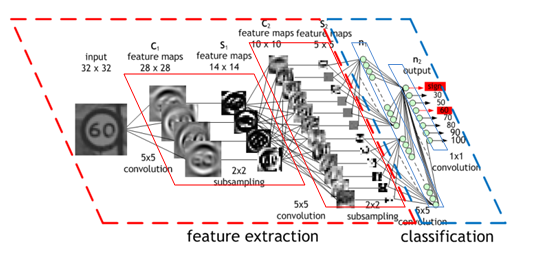
\includegraphics[scale=0.7]{convolutional_neural_network_structure} \]
  \centering
  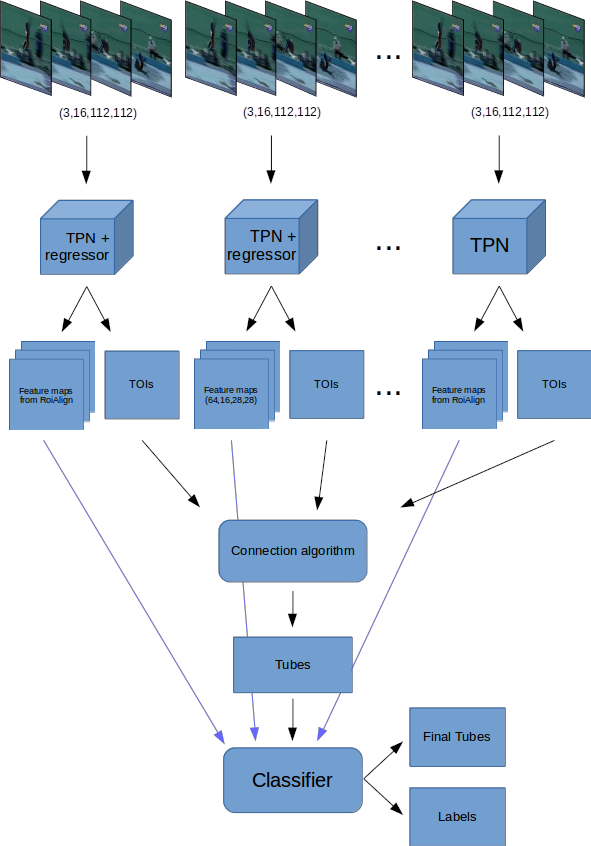
\includegraphics[scale=0.42]{model_prenms}
  \caption{The structure of the whole network}
  \label{fig:whole_network_}
\end{figure}

\section{Introduction to TPN}
 The main purpose of Tube Proposal Network (TPN)  is to propose
\textbf{Tube of Interest}(TOIs). These tubes are likely to contain an known action and are consisted of some 2D boxes
(1 for each frame). TPN is inspired from RPN introduced by FasterRCNN (\cite{Ren:2015:FRT:2969239.2969250}), but instead of images, TPN
is used in videos as performed by \cite{DBLP:journals/corr/HouCS17}. In full correspondence with RPN, the structure
of TPN is similar to RPN. The only difference, is that TPN uses 3D Convolutional Layers and 3D anchors instead of 2D. \par
We designed 2 main structures for TPN. Each approach has a different definition of the used 3D anchors.
The rest structure of the TPN is mainly the same with some little differences in the regression layer. \par

\section{Preparation before TPN}

\subsection{Preparing data}
Before getting a video as input to extract its features and ToIs, this video has to be preprocessed.
Preprocess procedure  is the same for both approaches of TPN.
Our architecture gets as input a sequence of frames which has a fixed  width, height and duration. However, each video has a different resolution. That's creates the
need to resize each frame before feeding it to the architecture.
As mentioned in the previous chapter, the first element of our network is a 3D ResNet taken from \cite{hara3dcnns}. This network is designed to
get images with dimensions (112,112). As a result, we resize each frame from datasets' videos into (112,112) frames. In order to keep aspect ratio, we pad each frame either
left and right, either above and bellow depending which dimension is bigger. In figure  \ref{fig:Preprocess_example} we can see the original frame and the resize and padded one.
In full correspondence, we resize the groundtruth bounding boxes for each frame (figure \ref{fig:original_image_rois} and \ref{fig:trans_image_rois} show that).

\begin{figure}[h]
  \centering
  \begin{subfigure}{0.35\textwidth}
    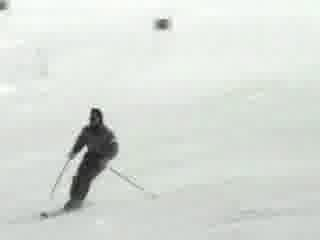
\includegraphics[width=\textwidth]{./figures/original_image.jpg}
    \caption{}
    \label{fig:original_image}
  \end{subfigure}
  \hfill
  \begin{subfigure}{0.35\textwidth}
    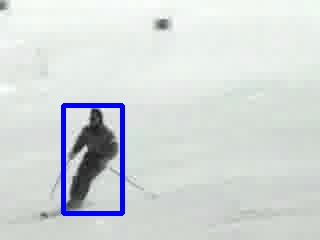
\includegraphics[width=\textwidth]{./figures/original_image_rois.jpg}
    \caption{}
    \label{fig:original_image_rois}
  \end{subfigure}
  \hfill
  \begin{subfigure}{0.35\textwidth}
    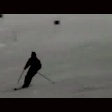
\includegraphics[width=\textwidth]{./figures/transformed_image.jpg}
    \caption{}
    \label{fig:trans_image}
  \end{subfigure}
  \hfill
  \begin{subfigure}{0.35\textwidth}
    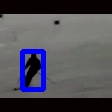
\includegraphics[width=\textwidth]{./figures/transformed_image_rois.jpg}
    \caption{}
    \label{fig:trans_image_rois}
  \end{subfigure}

  \caption{ At (a), (b) frame is its original size and at (c), (d) same frame after preprocessing part}
  \label{fig:Preprocess_example}
\end{figure}


\subsection{3D ResNet}
Before using the Tube Proposal Network, we extract spatiotemporal features of the video. In order to do so, we extract the 3 first Layers of a
pretrained 3D ResNet34. This Network is pretrained in Kinetics dataset \cite{DBLP:journals/corr/KayCSZHVVGBNSZ17} for sample duration
equal to 16  frames and sample size equal to (112, 122). \par
This network normally is used for classifying the whole video, so some of its layers use temporal stride equal to 2.
We set their temporal stride equal to 1 because we don't want to miss any temporal information during the process.
So, the output of the third layer is a feature maps with dimensions (256,16,7,7). We feed this feature map to TPN, which is described
in the following sections.

\section{ 3D anchors as 6-dim vector}
\subsection{First Description}
We started designing our TPN inspired by \cite{DBLP:journals/corr/HouCS17}. We consider each anchor as a 3D bounding box written as
$(x_1, y_1, t_1, x_2, y_2, t_2)$ where $x_1, y_1, t_1$
are the upper front left coordinates of the cuboid and $x_2, y_2, t_2$ are the lower back left as shown in figure \ref{fig:anchor_6d}.
\begin{figure}[h]
  \centering
  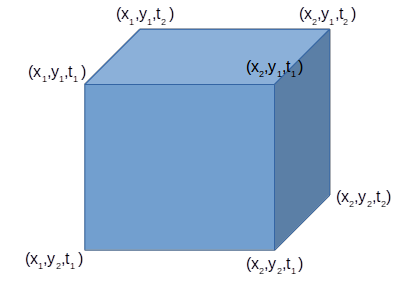
\includegraphics[scale=0.5]{anchor_6d}
  \caption{An example of the anchor $(x_1,y_1,t_1,x_2,y_2,t_2)$}
  \label{fig:anchor_6d}
\end{figure}

The main advantage of this approach is that, except from x-y dims, the dimension of time is mutable. As a result, the proposed TOIs have
no fixed time duration. This will help us deal with untrimmed videos, because proposed TOIs would exclude background frames.
For this approach, we use \textbf{n = 4k = 60} anchors for each pixel in the feature map of TPN. We have k anchors for each anchor 
duration( 5 scales of 1, 2, 4, 8, 16, 3 aspect ratios of 1:1, 1:2, 2:1 and 4 durations of 16,12,8,4 frames).
In \cite{DBLP:journals/corr/HouCS17},  network's anchors are defined according to the dataset most common anchors. This, however,
creates the need to redesign the network for each dataset. In our approach, we use the same anchors for both datasets, because we want our network not
to be dataset-specific but to be able to generalize for several datasets. As sample duration, we chose 16 frames per video segment because
our pre-trained ResNet is trained for video clips with that duration.
So the structure of TPN is:
\begin{itemize}
\item 1 3D Convolutional Layer with kernel size = 3, stride = 3 and padding = 1
\item 1 classification layer outputs \textit{2n scores,} whether there is an action or not for \textit{n tubes}.
\item 1 regression layer outputs \textit{6n coordinates} ($x_1,y_1,t_1,x_2,y_2,t_2$) for \textit{n tubes}.
\end{itemize}

The structure of TPN is shown in figure \ref{fig:tpn_1_1}. The output of TPN is the k-best scoring cuboid,which are most likely to contain an action.
\begin{figure}[h]

  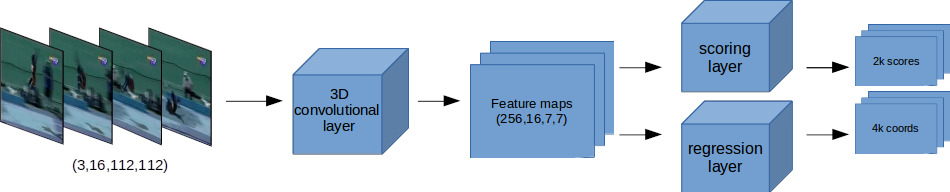
\includegraphics[width=1.\textwidth]{tpn_1_1}
  \caption{Structure of TPN}
  \label{fig:tpn_1_1}
\end{figure}

\subsection{Training}
As mentioned before, TPN extracts TOIs as 6-dim vectors. For that reason, we modify out groundtruth ROIs to groundtruth Tubes.
We take for granted that the actor cannot move a lot during 16 frames, so that's why we use this kind of tubes. As shown 
in figure \ref{fig:gt_tubes_and_rois}, these tubes are 3D boxes which include all the groundtruth rois, which are different
for each frame.

\begin{figure}[h]
  \centering
  \begin{subfigure}{0.15\textwidth}
    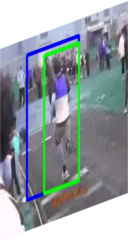
\includegraphics[width=\textwidth]{output/img_0.jpg}
  \end{subfigure}
  \begin{subfigure}{0.15\textwidth}
    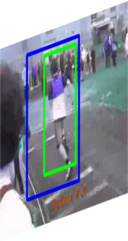
\includegraphics[width=\textwidth]{output/img_3.jpg}
  \end{subfigure}
  \begin{subfigure}{0.15\textwidth}
    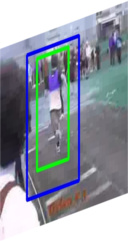
\includegraphics[width=\textwidth]{output/img_5.jpg}
  \end{subfigure}
  \begin{subfigure}{0.15\textwidth}
    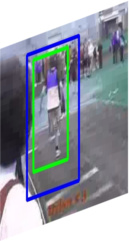
\includegraphics[width=\textwidth]{output/img_7.jpg}
  \end{subfigure}
  \begin{subfigure}{0.15\textwidth}
    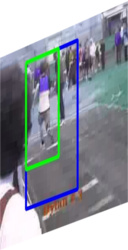
\includegraphics[width=\textwidth]{output/img_11.jpg}
  \end{subfigure}
  \begin{subfigure}{0.15\textwidth}
    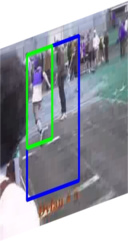
\includegraphics[width=\textwidth]{output/img_15.jpg}
  \end{subfigure}
  \caption{Groundtruth tube is colored with blue and groundtruth rois with color green}
  \label{fig:gt_tubes_and_rois}
\end{figure}

For training procedure, for each video, we randomly select a part of it which has duration 16 frames. We consider an anchor as foreground if its overlap score with a groundtruth
action tube is bigger than 0.5. Otherwise, it is considered as background anchor. We use scoring layer in order to correctly classify those anchors and we use
Cross Entropy Loss as loss function. We have a lot of anchors for proposing an action, but a small number of per-video actions, so we choose 256 anchors in total for each batch. We set the maximum
number of foreground anchors to be  25\% of the 256 anchors and the rest are the background.\par
Classifying correctly an anchor isn't enough for proposing an action tube. It is,also necessary, the anchors  overlap as much as possible with the groundtruth action tubes. That's the reason we use a
regression layer. This layer ``moves'' the cuboid closer to the area that it is believed that is closer to the action.
For regression loss we use smooth-L1 loss as proposed from \cite{DBLP:journals/corr/GirshickDDM13}. In order to calculate
the regression targets, we use pytorch FasterRCNN implementation (\cite{jjfaster2rcnn}) for bounding box regression and 
we modified the code in order to extend it for 3 dimensions. % \textbf{TODO more details}
So we have:
\[ \begin{matrix}
    t_x = (x-x_a)/w_a, & t_y = (y-y_a)/h_a, & t_z= (z-z_a)/d_a, \\
    t_w= log(w/w_a), & t_h= log(h/h_a), & t_d = log(d/d_a), \\
    t^*_x = (x^* - x_a)/w_a, & t^*_y = (y^* - y_a)/h_a, & t^*_z = (z^* - z_a)/d_a, \\
    t^*_w = log(w^* /w_a), & t^*_h = log(h^*/h_a), & t^*_d = log(d^*/d_a),
    % t∗x= (x∗−xa)/wa,  t∗y= (y∗−ya)/ha,t∗w= log(w∗/wa),  t∗h= log(h∗/ha)
  \end{matrix}
\]
where \textit{x, y, z, w, h, d} denote the 3D box's center coordinates and its width, height and duration. Variables $x, x_a, \text{ and } x^*$
are for the predicted box, anchor box, and groundthruth box respectively (likewise for \textit{y, z, w, h, d}). Of course, we calculate the
regression loss only for the foreground anchors and not for the background, so at the most we will calculate 64 targets
for each batch. \par

To sum up training procedure, we train 2 layers for our TPN, scoring and regression layers. The training loss includes the training losses
obtained by these layers and its formula is:
% \[ L  = \frac{1}{N_{cls}} \sum_iL_{cls}(p_i, p^*) + \frac{1}{N_{reg}}\sum_ip_i^*L_{reg}(t_i,t_i^*) \]
\[ L  =  \sum_iL_{cls}(p_i, p_i^*) + \sum_ip_i^*L_{reg}(t_i,t_i^*) \]
where:
\begin{itemize}
\item $L_{cls} $ is the Cross Entropy loss we use for classifying the anchors, with $p_i$ is the predicted label, $p_i^*$ is the groundtruth class and
  $p_i, p_i^* \in \{0,1\}$
\item $L_{reg} $ is the smooth-L1 loss function, which is multiplied  with $p_i^*$ in order to be set active only when there is a positive anchor $(p_i^* = 1)$
  and to be deactivated for background anchors $(p_i^* = 0)$.
\end{itemize}

\subsection{Validation}

Validation procedure is a bit similar to training procedure.
We randomly select 16 frames from a validation video and we examine if there is at least 1 proposed TOI
which overlaps $\ge$ 0.5 with each groundtruth action tube and we get recall score. 
In order to get good proposals, after getting classification scores and target prediction from the
corresponding layers, we use Non-Maximum Suppression (NMS) algorithm.  We set NMS threshold equal to 0.7,
and we keep the first 150 cuboids with the biggest score.

\subsection{Modified Intersection over Union(mIoU)} 
During training, we get numerous anchors. We have to classify them as foreground anchors or
background anchors. Foreground anchors are those which contain some action, and, respectively, background
don't. As presented before, IoU for cuboids calculates the ratio between the volume of overlap and volume of
union.
Intuitively, this criterion is good for evaluating 2 tubes if they overlap, but it has one big drawback:
it considers x-y dimensions to have the same importance with time dimension, which we do not desire. That's because
firstly we care to be accurate in time dimension, and then we can fix x-y domain.
As a result, we change the way we calculate the Intersection Over Union. We calculate separately
the IoU in x-y domain (IoU-xy) and in t-domain (IoU-t). Finally, we multiply them in order to get the final IoU.
So the formula for 2 tubes ($x_1, y_1, t_1, x_2, y_2, t_2$) and ($x'_1, y'_1, t'_1, x'_2, y'_2, t'_2$) is:
\[ IoU_{xy} = \frac{ \text{Area of Overlap in x-y}} { \text{Area of Union in x-y}}  \]
\[ IoU_t = \frac { max(t_1, t'_1) - min(t_2, t'_2)} {min(t_1,t'_1) - max(t_2,t'_2)} \]
\[ IoU = IoU_{xy} \cdot  IoU_t \]
The above criterion help us balance the impact of time domain in IoU. For example, let us consider 2 anchors:
a = (22, 41, 1, 34, 70, 5) and b = (20, 45, 2, 32, 72, 5). These 2 anchors in x-y domain have IoU score equal to 0.61.
But they are not exactly overlapped in time dimension. Using the first approach we get 0.5057 IoU score and using the
second approach we get 0.4889. So, the second criterion would reject this anchor, because there is a difference in time
duration.  \par

In order to verify our idea, we train TPN using both IoU and mIoU criterion for tube-overlapping. At Table \ref{table:iou_miou}
we can see the performance in each case for both datasets, JHMDB and UCF. The recall threshold for this case is 0.5 and during validation,
we use regular IoU for defining if 2 tubes overlap.
\begin{table}[h]
\centering
  \begin{tabular}{|| c | c || c ||}
    \hline
    \textbf{Dataset} & \textbf{Criterion} & \textbf{Recall(0.5)} \\
    \hline  \hline
    \multirow{2}{4em}{JHMDB} & IoU & 0.70525 \\
    \cline{2-3}
    {} & mIoU & 0.7052 \\
    \hline
    \multirow{2}{4em}{UCF} & IoU & 0.4665 \\
    \cline{2-3}
    {} & mIoU & 0.4829 \\
    \hline      
  \end{tabular}
  \caption{Recall results for both datasets using IoU and mIoU metrics}
  \label{table:iou_miou}
\end{table}

Table \ref{table:iou_miou} shows that modified-IoU give us slightly better recall performance only in UCF dataset. That's reasonable, because JHMDB dataset
uses trimmed videos so time duration doesn't affect a lot. So, from now own, during training we use mIoU as overlapping scoring policy.

\subsection{Improving TPN score}
After first tests, we came with the idea that in a video lasting 16 frames, in time domain, all kinds of actions can be separated into the following categories:
\begin{enumerate}
\item The action starts in the n-th  frame and finishes after the 16th frame of the sampled video.
\item The action has already begun before the 1st frame of the video and ends in the n-th frame.
\item The action has already begun before the 1st frame of the video and finishes after the 16th video frame.
\item The action starts and ends in that 16 frames of the video.
\end{enumerate}

On top of that, we noticed that most of actions, in our datasets, last more that 16 frames. So, we came with the idea to add  1 scoring layer and 1 regression layer
which will propose ToIs with fixed duration equal to the sample duration (16 frames) and they will take into account the spatial information produced by activation maps.
The new structure of TPN is shown in figure \ref{fig:tpn_1_2}. After getting proposals from both scores, we concat them with ratio 1:1 between ToI extracted
from those 2 subnetworks.

\begin{figure}[h]
  \centering
  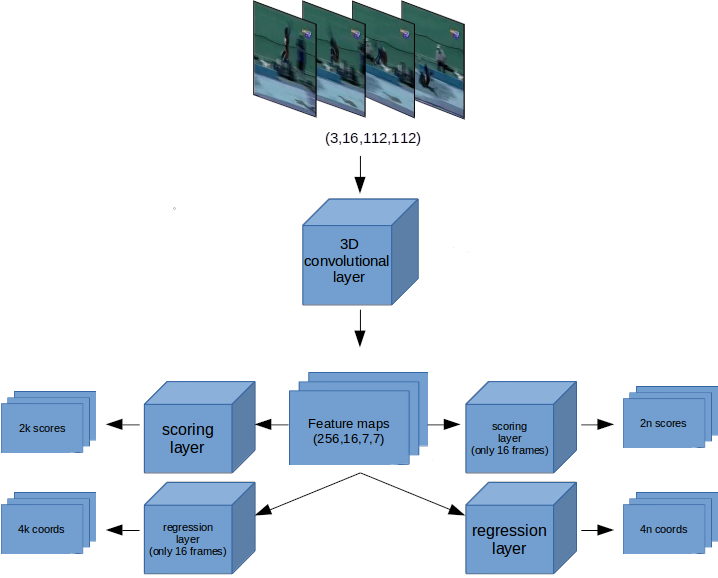
\includegraphics[scale=0.5]{tpn_1_2}
  \caption{TPN structure after adding 2 new layers, where k = 5n.}
  \label{fig:tpn_1_2}
\end{figure}
Our goal is to ``compress'' feature maps in the temporal dimension in order to propose ToIs based only on the spatial information.
So, we came with 2 techniques for doing such thing:
\begin{enumerate}
\item Use 3D Convolutional Layers with kernel size = (sample duration, 1,1), stride =1 and no padding for scoring and regression.
  This kernel ``looks'' only in the temporal dimension of the activation maps and doesn't consider any spatial dependencies.
\item Get the average values from temporal dimension and then use a 2D Convolutional Layer for scoring and regression.
\end{enumerate}

% \textbf{TODO na perigrapsw oti thelw na exw ola ta xronika features}
\par
Training and Validation procedures remain the same. The only big difference is that now we have losses obtained from 2 different systems which propose TOIs. On top of that,
during validation, we,at first, concate proposed ToIs and, then, we follow the same procedure, which is calculating recall performance. For training loss, we have 2 different cross-entropy losses and 2 different smooth-L1 losses, each for every
layer correspondingly. So training loss is, now, defined as :

  % \begin{aligned}
 % L  =  \sum_iL_{cls}(p_i, p_i^*) + \sum_iL_{cls}(p_{fixed,i}, p_{fixed,i}^*) +  
 %  \sum_ip_i^*L_{reg}(t_i,t_i^*) + \sum_ip_{fixed,i}^*L_{reg}(t_{fixed,i},t_{fixed,i}^*) 
% L  =2


% \[ L  =  \sum_iL_{cls}(p_i, p_i^*) + \sum_iL_{cls}(p_{fixed,i}, p_{fixed,i}^*) +  \newline
%   \sum_ip_i^*L_{reg}(t_i,t_i^*) + \sum_ip_{fixed,i}^*L_{reg}(t_{fixed,i},t_{fixed,i}^*) \]
% \end{aligned}


\begin{equation} 
\begin{split}
 L  =  \sum_iL_{cls}(p_i, p_i^*) + \sum_iL_{cls}(p_{fixed,i}, p_{fixed,i}^*) + \\
   \sum_ip_i^*L_{reg}(t_i,t_i^*) + \sum_ip_{fixed,i}^*L_{reg}(t_{fixed,i},t_{fixed,i}^*) 
  % \sum_iL_{cls}(p_i, p_i^*) + \sum_iL_{cls}(p_{fixed,i}, p_{fixed,i}^*) 
\end{split}
\end{equation}

where:
\begin{itemize}
  \item $L_{cls} $ is the Cross Entropy loss we use for classifying the anchors, with $p_i$ is the predicted label, $p_i^*$ is the groundtruth class and
  $p_i, p_i^* \in \{0,1\}$
\item $L_{reg} $ is the smooth-L1 loss function, which multiply it with $p_i^*$ in order to set active only when we have a positive anchor $(p_i^* = 1)$
  and to be deactivated for background anchors $(p_i^* = 0)$.
\item $p_i $ are the anchors from scoring and regression layers with mutable time duration and $p_i^*$ are their corresponding groundtruth label.
\item $p_{fixed,i} $ are the anchors from scoring and regression layers with fixed time duration = 16 and $p_{fixed,i}^*$ are their corresponding groundtruth label.
\end{itemize}

We train our TPN Network using both techniques and their recall performance is shown in Table \ref{table:add_16}.

\begin{table}[h]
  \centering
  \begin{tabular}{||c | c | c || c ||}
    \hline
    \textbf{Dataset} & \textbf{Fix-time anchors} & \textbf{Type} & \textbf{Recall(0.5)} \\
    \hline  \hline
    \multirow{3}{4em}{JHMDB} & No &  - & 0.7052 \\
    \cline{2-4}
    {} & \multirow{2}{*}{Yes} & Kernel & 0.6978 \\
    \cline{3-4}
    {} & {} & Mean & 0.7463 \\
    \hline
    \multirow{3}{4em}{UCF} & No & - & 0.4829 \\
    \cline{2-4}
    {} & \multirow{2}{*}{Yes} & Kernel & 0.4716 \\
    \cline{3-4}
    {} & {} & Mean & 0.4885 \\
    \hline      
  \end{tabular}
  \caption{Recall results after adding fixed time duration anchors}
  \label{table:add_16}
\end{table}

As we can see from the previous results, the new layers increased recall performance significantly. On top of that, Table \ref{table:add_16} shows that
getting the average values from the time dimension gives us the best results.


\subsection{Adding regressor}
The output of TPN is the $\alpha$-highest scoring anchors moved according to their regression prediction. After that, we have to turn the proposed anchors into ToIs.
In order to do so, we add a regressor system which gets as input cuboids' feature maps and returns a sequence of 2D boxes, one per every frame.
The only problem is that the regressor needs as input feature maps with fixed size . This problem is already solved by R-CNNs which use roi pooling and roi align
in order to get fixed size feature maps from ROIs with changing sizes. In our situation, we extend roi align operation, presented by Mask R-CNN(\cite{DBLP:journals/corr/HeGDG17}),
and we
call it \textbf{3D Roi Align}.

\paragraph{3D Roi Align}
3D Roi align is a modification of roi align presented by Mask R-CNN . The main difference between those two is that Mask R-CNN's roi align uses
bi-linear interpolation for extracting ROI's features and ours 3D roi align uses trilinear interpolation for the same reason. Again, the 3rd dimension is
time.
So, we have as input a feature map extracted from ResNet34 with dimensions (64,16,28,28) and a tensor containing the proposed TOIs.
For each TOI whose activation map has size equal to (64,16,7,7), we get as output a feature map with size (64, 16, 7, 7). \par

\subsubsection{Regression procedure}
At first, for each proposed ToI, we get its corresponding activation maps using 3D Roi Align. These features are given as input to a regressor. This regressor returns 16 $\cdot$ 4 predicted
transforms $(\delta_x,\delta_y, \delta_w,\delta_h)$, 4 for each frame, where $ \delta_x, \delta_y$ specify the coordinates of proposal's center and $\delta_w, \delta_h$ its width and height, as specified
in \cite{DBLP:journals/corr/GirshickDDM13}.  We keep only the predicted translations, for the frames that are $\ge t_1$ and $< t_2$ and for the other frames, we set a zero-ed 2D box. 
After that, we modify each anchor from a cuboid written like $(x_1,y_1,t_1, x_2, y_2, t_2)$ to a sequence of 2D boxes, like: \\
$(0,0,0,0, ..., x_{T_1},y_{T_1},x'_{T_1},y'_{T_1}, ... ,x_{i},y_{i},x'_{i}, ..., x_{T_2},y_{T_2},x'_{T_2},y'_{T_2}, 0,0,0,0, ....)$, \\
where:
\begin{itemize}
\item $ T_1 \le i \le T_2$, for $T_1 < t_1 + 1,  T_2 < t_2 \text{ and }T_1,T_2 \in \mathbb{Z} $
\item $ x_i = x_1, y_i= y_1, x'_i = x_2, y'_i = y_2 $.
\end{itemize}

\paragraph{ Training}
In order to train our Regressor, we follow about the same steps followed previously for previous TPN's training procedure. This means that
we randomly pick 16 ToI from those proposed by TPN's scoring layer. From those 16 tubes, 4 are foreground tubes, which means 25\% of the total
number of the tubes as happened previously. We extract their corresponding features using 3D Roi Align and calculate their targets like
we did for regression layer. We feed Regressor Network with these features and compare the predicted targets with the expected.
Again, we use smooth-L1 loss for loss function, calculated only for foreground ToIs. So, we add another parameter in
training loss formula which is now defined as:
% \textbf{TODO Describe training procedure}
% \textbf{TODO Training Loss formula}
\begin{equation} 
\begin{split}
 L  =  \sum_iL_{cls}(p_i, p_i^*) + \sum_iL_{cls}(p_{fixed,i}, p_{fixed,i}^*) + \\
 \sum_ip_i^*L_{reg}(t_i,t_i^*) + \sum_ip_{fixed,i}^*L_{reg}(t_{fixed,i},t_{fixed,i}^*) + \\
  \sum_iq_i^*L_{reg}(c_{i}, c_{i}^*) + \\
  % \sum_iL_{cls}(p_i, p_i^*) + \sum_iL_{cls}(p_{fixed,i}, p_{fixed,i}^*) 
\end{split}
\end{equation}
where  except the previously defined parameters, we set  $c_{i} $ as the regression targets for picked tubes $q_i$.
These tubes are the ones randomly selected from the proposed ToIs and $q_i^*$ are their corresponding groundtruth action tubes, which are the closest to each $q_i$ tube.
Again, we use $q_i^*$ as a factor because we consider a tube as background when it doesn't overlap with any groundtruth action tube more that 0.5 .

\subsubsection{First regression Network} 

The architecture of reggression network is shown in Figure \ref{fig:regressor_3d}, and it is described below:
\begin{figure}[h]
  \centering
  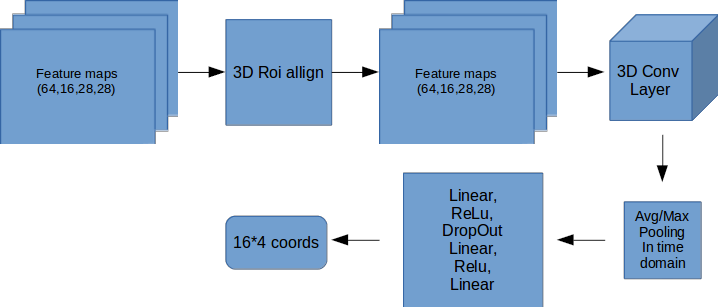
\includegraphics[scale=0.48]{regressor_1_1}
  \caption{Structure of Regressor}
  \label{fig:regressor_3d}
\end{figure}

\begin{enumerate}
\item Regressor is consisted, at first, with a 3D convolutional layer with kernel = 1, stride = 1 and no padding. This layer gets as input ToI's normalized activation map extracted from 3D Roi Align.
\item After that, we calculate the average value in time domain, so from a feature map with dimensions (64,16,7,7), we get as output a feature map (64,7,7).
\item These feature maps are given as input to a Linear layer, followed by a Relu Layer, a Dropout Layer, another Linear Layer and Relu Layer and a final Linear.
\end{enumerate}

We use Recall metric In order to assess the performance of regressor. We calculate 3 recall performances:
\begin{description}
\item [Cuboid Recall,] which is the recall performance for proposed cuboids. We interested in this metric because, we
  want to know how good are our proposals before modifying them into sequences of boxes.

\item [Single frame Recall,] which is the recall performance for the proposed ToI against the groundtruth tubes.
\item[Follow-up Single Frame Recall,] which is the recall performance for only the cuboids that were over the overlap threshold between
  proposed cuboids and groundtruth cuboids. We use this metric in order to know how many of our proposed cuboids end up in being good proposals.
\end{description}

\begin{table}[h]
  \centering
  \begin{tabular} {||c | c || c | c | c ||}
    \hline
    \textbf{Dataset} & \textbf{Pooling} & \textbf{Cuboid} & \textbf{Singl. Fr. } &  \textbf{Follow-up S.F.}\\
    \hline                
    \multirow{2}{*}{JHMDB} & avg & 0.8545 & 0.7649 & 0.7183 \\
    \cline{2-5}
    {} & max & 0.8396 & 0.7761 & 0.5783 \\
    \cline{1-5}
    \multirow{2}{*}{UCF} & avg & 0.5319 & 0.4694 & 0.5754 \\
    \cline{2-5}
    {} & max & 0.5190 & 0.5021 & 0.5972 \\
    \cline{1-5}
                                   
  \end{tabular}
  \caption{Recall results after converting cuboids into sequences of frames}
  \label{table:reg_1_1}
\end{table}

As the above results show, we get lower recall performance in frame-level. On top of that, when we translate a cuboid into
a sequence of boxes, we miss 20-40\% of our proposals. This means that we don't modify good enough our cuboids, although
we get only 10\% decrease. Probably, we get such score from cuboids, that even though, didn't overlap well (according to
overlap threshold), achieve to become a good proposal in frame-level and in temporal level. 


\subsection{Changing Regressor - from 3D to 2d}
After getting first recall results, we experiment using another architecture for the regressor network, in order to solve the modification
problem, introduced in the previous section. Instead of having a 3D Convolutional Layer, we will use a 2D Convolutional Layer
in order to treat the whole time dimension as one during convolution operation. So, as shown in Figure \ref{fig:reg_1_2},
the $2^{nd}$ Regression Network is about the same with first one, with 2 big differences:
\begin{enumerate}
\item We performing a pooling operation at the feature maps extracted by the 3D Roi Align operation, after we are normalized.
\item Instead of a 3D Convolutional Layer, we have a 2D Convolutional Layer with kernel size = 1, stride = 1 and no padding.
\end{enumerate}

\begin{figure}[h]

  \centering
  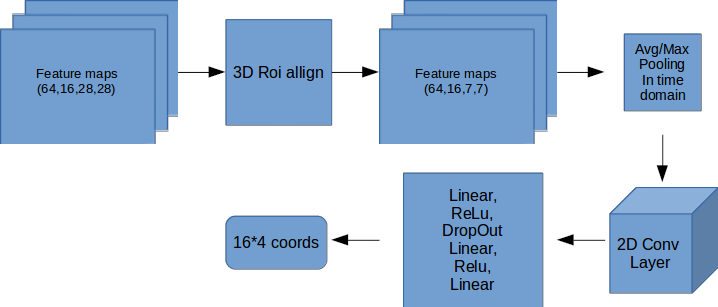
\includegraphics[scale=0.48]{regressor_1_2}
  \caption{Structure of Regressor}
  \label{fig:reg_1_2}
\end{figure}

On top of that, we tried to determine which feature map is the most suitable  for getting best-scoring recall performance. This feature map will be given as
input to the Roi Algin operation.  At Table \ref{table:reg_1_2}, we can see the recall performance for different feature maps and different pooling methods.

\begin{table}[h]
  \centering
  \begin{tabular}{||c | c | c || c  c  c ||}
    \hline
    \textbf{Dataset} & \textbf{Pooling} & \textbf{F. Map} & \textbf{Recall} &  \textbf{ Recall SR}  &  \textbf{Recall SRF} \\
    \hline
    \multirow{6}{*}{JHMDB} & \multirow{3}{*}{mean} & 64 &  0.6828  & 0.5112  & 0.7610 \\
    \cline{3-6}
    {} & {} & 128 & 0.8694 & 0.7799 & 0.6756 \\
    \cline{3-6}
    {} & {} & 256 & 0.8396 & 0.7687 & 0.7029 \\
    \cline{2-6}
    {} & \multirow{3}{*}{max} & 64 &  0.8582 & 0.7985 & 0.5914\\
    \cline{3-6}
    {} & {} & 128 & 0.8358 & 0.7724 & 0.8118 \\
    \cline{3-6}
    {} & {} & 256 & 0.8657 & 0.8022 & 0.7996 \\
    \hline
    \multirow{6}{*}{UCF} & \multirow{3}{*}{mean} & 64 & 0.5055 & 0.4286 & 0.5889 \\
    \cline{3-6}
    {} & {} & 128 & 0.5335 & 0.4894 & 0.5893 \\
    \cline{3-6}
    {} & {} & 256 & 0.5304 & 0.4990 & 0.6012 \\
    \cline{2-6}
    {} & \multirow{3}{*}{max} & 64 & 0.5186 & 0.4990 & 0.5708 \\
    \cline{3-6}
    {} & {} & 128 & 0.5260 & 0.4693 & 0.5513 \\
    \cline{3-6}
    {} & {} & 256 & 0.5176 & 0.4878 & 0.6399 \\
    \hline

  \end{tabular}
  \caption{Recall performance using 3 different feature maps as Regressor's input and 2 pooling methods}
  \label{table:reg_1_2}
\end{table}

As we noticed from the above results, again, our system has difficulty in translating cuboids into 2D sequence of ROIs.
So, that makes us rethink the way we designed our TPN.


\section{ 3D anchors as 4k-dim vector}
In this approach, we set 3D anchors as 4k coordinates (k = 16 frames = sample duration). So a typical anchor is written as ($x_1, y_1, x'_1, y'_1, x_2, y_2, ...$)
where $x_1, y_1, x'_1, y'_1 $ are the coordinates for the 1st frame, $x_2, y_2, x'_2, y'_2$ are the coordinates for the 2nd frame etc, as presented in \cite{DBLP:journals/corr/abs-1712-09184}.
In figure \ref{fig:anchor_4k} we can an example of this type of anchor.

\begin{figure}[h]
  \centering
  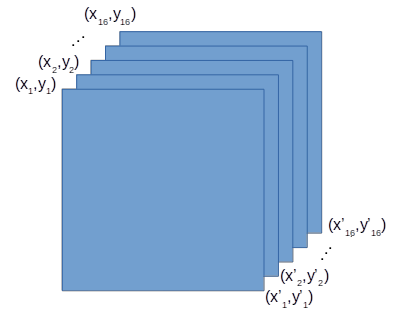
\includegraphics[scale=0.5]{anchor_4k}
  \caption{An example of the anchor $(x_1,y_1,x'_1,y'_1,x_2,y_2, ...)$}
  \label{fig:anchor_4k}
\end{figure}

The main advantage of this approach is that we don't need to translate the 3D anchors into 2D boxes, which caused many problems at the previous approach.
However, it has a big drawback, which is the fact that this type of anchors has fixed time duration.
In order to deal with this problem, we set anchors with different time durations, which are 16, 12, 8 and 4.
Anchors with duration $ < $ sample duration (16 frames) can be written as 4k vector with zeroed coordinates in the frames bigger that the time duration. For example, an anchor with
2 frames duration, starting from the 2nd frame and ending at the 3rd can be written as (0, 0, 0, 0, $x_1, y_1, x'_1, y'_1, x_2, y_2, x'_2, y'_2$, 0, 0, 0, 0) if the sample
duration is 4 frames. 

\begin{figure}[h]
  \centering
  % 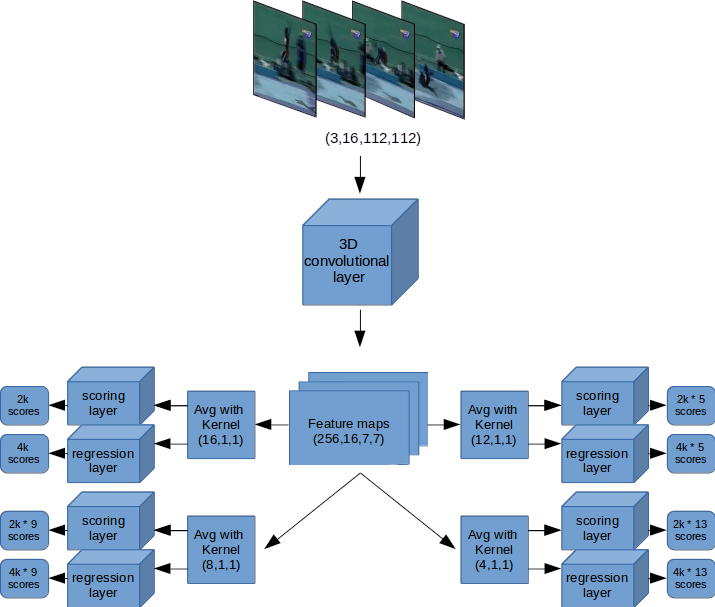
\includegraphics[width=1.\textwidth]{tpn_2}
  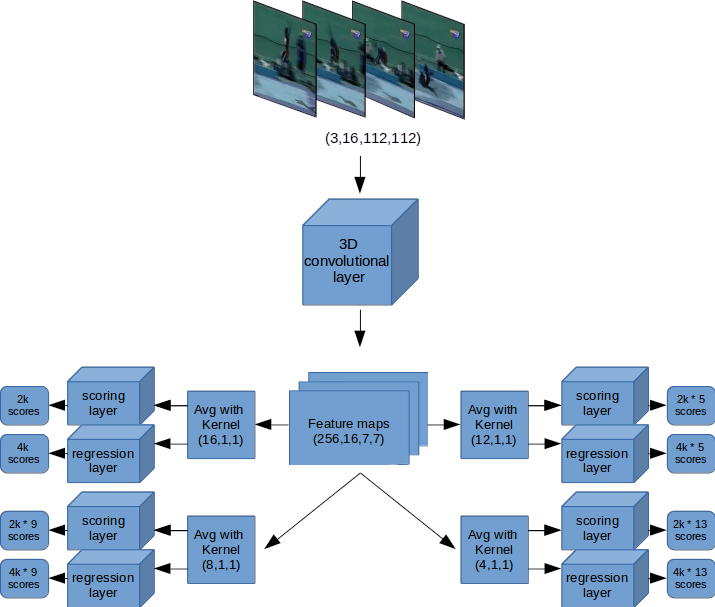
\includegraphics[scale=0.4]{tpn_2}
  \caption{The structure of TPN according to new approach}
  \label{fig:New_structure}
\end{figure}

This new approach led us to change the structure of TPN. The new one  is presented in figure \ref{fig:New_structure}. As we can see, we \
added scoring and regression layers for each duration. So, TPN follows the upcoming steps in order to propose ToIs:
\begin{enumerate}
\item At first, we get the feature map, extracted by ResNet, as input to a 3D Convolutional Layer with kernel size = 1, stride = 1 and no padding.
\item From Convolutional Layer, we get as output an activation map with dimensions (256,16,7,7). For reducing time dimension, we use 4 pooling layer,
  one for each sample duration with kernel sizes \textit{(16,1,1), (12,1,1,), (8,1,1) and (4,1,1)} and stride = 1,  for sample durations 16, 12, 8 and 4 respectively.
  So, we get activation maps with dimensions \textit{(256,1,7,7), (256,5,7,7), (256,9,7,7) and (256,13,7,7)}, in which second dimension is the number of possible
  time variations. For example, in $(256,5,7,7)$ feature map, which is related with anchors with duration 12 frames, we can have 5 possible cases, from frame 0 to frame
  11, frame 1 to frame 12 etc.
  
\item Again, like in previous approach, for each pixel of the activate map we correspond \textbf{n = k = 15}
  anchors (5 scale of 1, 2, 4, 8, 16, 3 aspect rations of  1:1, 1:2, 2:1). Of course, we have 4 different activate maps, with 1, 5, 9 and 13
  different cases and a $7 \times 7$ shape in each filter. So, in total we have $28 \cdot 15 \cdot 49 = 20580$ different anchors.
  Respectively, we have 20580 different regression targets.

\end{enumerate}

\subsection{Training}
Training procedure stays almost the same like previous approach's. So, again, we randomly choose  a video segment and its corresponding groundtruth action tubes. But in this training procedure,
we consider anchors as foreground when they overlap more than 0.7 with any groundtruth tube, alongside with background anchors whose overlap is bigger that 0.1 and smaller than 0.3. We are not
concerned about the rest of the anchors.

\begin{table}[h]
  \centering
  \begin{tabular}{||c | c || c  c c||}
    \hline
    \textbf{Dataset} & \textbf{Pooling} &  \textbf{Recall(0.5)} & \textbf{Recall(0.4)} & \textbf{Recall(0.3)} \\
    \hline  \hline
    \multirow{2}{4em}{JHMDB} & mean & 0.6866 & 0.7687 & 0.8582 \\
    \cline{2-5}
    {} & max &  0.8134 & 0.8694 & 0.9216 \\
    \hline
    \multirow{2}{4em}{UCF} & avg &  0.5435 & 0.6326 & 0.7075 \\
    \cline{2-5}
    {} & max & 0.6418 & 0.7255 & 0.7898 \\
    \hline
  \end{tabular}
  \caption{Recall results using 2nd approach for anchors}
  \label{table:tpn_2_1}
\end{table}

As Table \ref{table:tpn_2_1} shows, it is obvious that we get better recall performances compared to previous' approach.
Additionally, we can see that 3D max pooling performs better than 3D avg pooling. The difference
between max pooling and avg pooling is about 10\%, which is big enough to make us choose max pooling operation as pooling method before getting anchors' scores
and regression targets.

\subsection{Adding regressor}

Even though, our TPN outputs frame-level boxes, we need to improve these predictions in order to overlap
with the groundtruth boxes as well as possible.
So, in full correspondence with the previous approach, we added an regressor for trying to get better recall results.

\paragraph{3D Roi align}
In this approach, we know already the 2D coordinates. So, we can use the method proposed from \cite{DBLP:journals/corr/abs-1712-09184}. They
extend RoiAlign operator by splitting the tube into $T$ 2D boxes. Then, they use classic RoiAlign to extract a region from each one 
of the temporal slices in the feature map. After that, they concatenate the region in time domain so they get a $T \times R \times R$
feature map, where $R$ is the output resolution of RoiAlign, which is 7 in our situation. \par

As a first approach, we use a 3D convolutional layer, followed by 2 linear layers. Our regressors follows the following steps:
\begin{enumerate}
\item At first, use 3D RoiAlign in order to extract the feature maps of the proposed action tubes. We normalize them, and give them as input to the 3D
  convolutional layer.
\item The output of the 3D Convolutional Layer is fed into 2 Linear layers with ReLu faction between them and finally we get $sample duration \times 4$
  regression targets. We keep only the proposed targets, that there is a corresponding 2D box.
\end{enumerate}


We train our regressor using the same loss function as previous approach's formula which is:
\begin{equation*} 
\begin{split}
 L  =  \sum_iL_{cls}(p_i, p_i^*) + \sum_iL_{cls}(p_{fixed,i}, p_{fixed,i}^*) + \\
 \sum_ip_i^*L_{reg}(t_i,t_i^*) + \sum_ip_{fixed,i}^*L_{reg}(t_{fixed,i},t_{fixed,i}^*) + \\
  \sum_iq_i^*L_{reg}(c_{i}, c_{i}^*) + \\
  % \sum_iL_{cls}(p_i, p_i^*) + \sum_iL_{cls}(p_{fixed,i}, p_{fixed,i}^*) 
\end{split}
\end{equation*}

We want again to find the best matching feature maps, so we train our regressor for feature maps
$(64,8,7,7)$ and $(128,8,7,7)$. We didn't experiment using $(256,8,7,7)$ feature map because
we got OutOfMemory error during training, despite several modifications we did in the
implementation code.

\begin{table}[h]
  \centering
  \begin{tabular}{||c | c || c  c  c||}
    \hline
    \textbf{Dataset} & \textbf{Feat. Map} & \textbf{Recall(0.5)} & \textbf{Recall(0.4)} & \textbf{Recall(0.3)}\\
    \hline
    \multirow{2}{*}{JHMDB} &  64 & 0.7985 & 0.903 & 0.9552 \\
    \cline{2-5}
    {} & 128 & 0.7836 & 0.8881 & 0.944\\
    \hline
    \multirow{2}{*}{UCF}  & 64 & 0.5794 & 0.7206 & 0.8134 \\
    \cline{2-5}
    {} & 128 & 0.5622 & 0.7204 & 0.799 \\
    \hline

  \end{tabular}
  \caption{Recall performance when using a 3D Convolutional Layer in Regressor's architecture}
  \label{table:reg_2_1}
\end{table}

According to Table \ref{table:reg_2_1}, we got the best results when we use $(64,16,7,7)$ feature map. This is the expected result, because these feature maps
are closer to the actual pixels of the actor, than $(128,16,7,7)$ feature maps, in which because of $3 \times 3 \times 3$ kernels, which combine spatiotemporal
information from neighbour pixels. However, as we can see, we got worst recall performance than when we didn't use any regressor if we compare the results from Tables
\ref{table:tpn_2_1} and \ref{table:reg_2_1}.

\subsection{From 3D to 2D}

Following the steps we used before, we design an architecture that uses instead of a 3D Convolutional Layer, a 2D. Unlike we did before, in this case, we haven't 
used any pooling operation before feeding the first 2D Convolutional Layer. On the contrary, we manipulate our feature maps like not being spatiotemporal but,
only spatial. So, our steps are:
\begin{enumerate}
\item At first, we use, again ,3D RoiAlign in order to extract the feature maps of the proposed action tubes and normalize them. Let us consider a feature map
  extracted from ResNet, which has dimensions $(64,sample duration,7,7)$ and after applying RoiAlign and normalization, we get a $(k,64,sample duration,7,7)$ feature map,
  where \textit{k} is the number of proposed  action tubes for this video segment.
\item We slice the proposed action tubes into T 2D boxes, so the dimensions of the Tensor, which contains the coordinates of action tubes, from $(k,4\cdot sample duration)$
  become $(k,sample duration, 4)$. We reshape the Tensor into $(k\cdot sample duration, 4)$, in which, first k coordinates refer to the first frame, the
  second k coordinates refer to the second frame and so on.
\item Respectively, we reshape extracted feature maps from $(k, 64, sample duration, 7, 7)$ to $(k\cdot sample duration, 64, 7, 7)$. So, now we deal with 2D feature maps, for which as we said before,
  we consider that contain only spatial information. So, we use 3 Linear Layers in order to get 4 regression targets. We keep only those we have a corresponding bounding
  box.
\end{enumerate}

Again, we experiment using 64, 128 and 256 feature maps (in this case, there is no memory problem). The results of our experiments are shown in Table \ref{table:reg_2_2}.
% After getting first recall results, we experiment using another architecture for the regressor network. Our idea was that we can treat feature maps like not having
% temporal dependencies between their frames. So, at first, we get from Roi Align operation activation maps with dimensions \textit{(k,64,16,7,7)} where k is the number
% of ToIs proposed for this video segment. We reshape this feature map to \textit{ (k*16,64,7,7) }, and in same time, we reshape their proposed action tubes from \textit{(k,16,4)}
% to \textit{(k*16,4)}. So, the new regression Network is consisted with:
% % \begin{enumerate}
% % \item a 2D Convolutional Network
% \paragraph{From 3D to 2d}
% The first idea we thought, was to change the first Convolutional layer from 3D to 2D. This means that we consider  features  not to have temporal dependencies for
% each frame. As we can see in the figure \ref{}, we got worse results, so, we rejected this idea.

% \subsection{Trying to  improve performance}
% TODO
% \subsection{Changing training procedure}
% TODO

\begin{table}[h]
  \centering
  \begin{tabular}{||c | c || c  c  c||}
    \hline
    \textbf{Dataset}  & \textbf{Feat. Map} & \textbf{Recall(0.5)} & \textbf{Recall(0.4)} & \textbf{Recall(0.3)}\\
    \hline
    \multirow{3}{*}{JHMDB} & 64 & 0.8358 & 0.9216 & 0.9739\\
    \cline{2-5}
    {} & 128 & 0.8172 & 0.9142 & 0.9627 \\
    \cline{2-5}
    {} & 256 & 0.7724 & 0.8731 & 0.9328 \\
    \hline
    \multirow{3}{*}{UCF} & 64 & 0.6368 & 0.7346 & 0.7737 \\ 
    \cline{2-5}
    {} & 128 & 0.6363 & 0.7133 & 0.7822 \\
    \cline{2-5}
    {} & 256 &  0.6363 & 0.7295 & 0.7822 \\
    \hline

  \end{tabular}
  \caption{Recall performance when using a 2D Convolutional Layer instead of 3D in Regressor's model}
  \label{table:reg_2_2}
\end{table}

As we can see, we get improved recall performance up 3\% for JHMDB dataset and about the same performance for UCF dataset. Again, we get best performance
if we choose $(64, 16, 7, 7)$ feature maps.

\subsection{Changing sample duration}
After trying all the previous versions, we noticed that we get about the same recall performances with some small improvements. So, we thought that we could try
to reduce the sample duration. This idea is based on the fact that reducing sample duration, means that anchor dimensions will reduce, so the number of
candidate anchors. That's because, now we have a smaller number of cases, so smaller number of parameters alongside with a small number of dimensions for regression targets.
We train our TPN for sample duration = 8 frames 4 frames. We use, of course, TPN's second  architecture, because as shown before, we get better recall performance.

\subsubsection{Without Regressor}

At first, we train TPN, again without regressor. We do so, in order to compare recall performance for all sample durations, without using any regressor. The results
are shown in Table \ref{table:new_sample}. For all cases, we use max pooling before scoring and regression layers, and we didn't experiment at all with
avg pooling. Of course, for sample duration = 16, we used the calculated one in  Table \ref{table:tpn_2_1}.

\begin{table}[h]
  \centering
  \begin{tabular}{|c | c || c c c|}
    \hline
    \textbf{Dataset} & \textbf{Sample dur} & \textbf{Recall(0.5)} &  \textbf{Recall(0.4)} &  \textbf{Recall(0.3)} \\
    \hline
    \multirow{3}{*}{JHMDB} & 16 & 0.8134 & 0.8694 & 0.9216 \\
    \cline{2-5}
    {} & 8 & 0.9515 & 0.9888 & 1.0000 \\
    \cline{2-5}
    {} & 4 & 0.8843 & 0.9627 & 0.9888 \\
    \hline
    \multirow{3}{*}{UCF} & 16 & 0.6418 & 0.7255 & 0.7898 \\
    \cline{2-5}
    {} & 8 & 0.7942 & 0.8877 & 0.9324\\
    \cline{2-5}
    {} & 4 & 0.7879 & 0.8924 & 0.9462 \\
    \hline
    
  \end{tabular}
  \caption{Recall results when reducing sample duration to 4 and 8 frames per video segment}
  \label{table:new_sample}
\end{table}

According to Table \ref{table:new_sample}, we notice that we get best performance for sample duration = 8 for both datasets. For dataset JHMDB sample duration equal to 8
gets far better results from the other approaches, followed by approach with sample duration = 4. For UCF dataset, although sample duration equal to 8 gives us best performances
sample duration equal to 4 gives us about the same. The difference between those 2 duration is less that 1\%. 

\subsubsection{With Regressor}                                             

Following the idea of reducing the sample duration for getting better recall performance, we trained TPN with a regressor. We trained for both approaches, which means both 3D and 2D Convolutional
Layer approaches were trained. Recall performances are presented in Table \ref{table:new_sample_reg}.

\begin{table}[h]
  \centering
  \begin{tabular}{|c | c | c || c c c|}
    \hline
    \textbf{Dataset} & \textbf{Sample dur} & \textbf{Type} & \textbf{Recall(0.5)} &  \textbf{Recall(0.4)} &  \textbf{Recall(0.3)} \\
    \hline
    \multirow{4}{*}{UCF} & \multirow{2}{*}{8} & 2D & 0.8078 & 0.8870 & 0.9419 \\
    \cline{3-6}
    {} & {} & 3D & 0.8193 & 0.8930 & 0.9487 \\
    \cline{2-6}
    {} & \multirow{2}{*}{4}& 2D & 0.7785 & 0.8914 & 0.9457 \\
    \cline{3-6}
    {} & {} & 3D & 0.7449 & 0.8605 & 0.9362 \\
    \hline
    \multirow{4}{*}{JHDMBD} & \multirow{2}{*}{8} & 2D &  0.9366 & 0.9851 & 0.9925  \\
    \cline{3-6}
    {} & {} & 3D & 0.8918 & 0.9776 & 0.9963  \\ 
    \cline{2-6}
    {} & \multirow{2}{*}{4}& 2D & 0.9552 & 0.9963 & 1.0000 \\
    \cline{3-6}
    {} & {} & 3D & 0.9142 & 0.9701 & 0.9888  \\
    \hline
    
  \end{tabular}
  \caption{Recall results when a regressor and sample duration equal to 4 or 8 frames per video segment}
  \label{table:new_sample_reg}
\end{table}

According to \ref{table:new_sample_reg}, it is clear that using a 2D Convolutional Layer as presented above results in better recall performance that using a 3D. Furthermore, we notice that
the addition of a regressor causes both improvements and deteriorations in recall performances. For dataset UCF, approach with sample duration = 8 improves by about 1-2\% recall performance,
but for sample duration = 4 it reduce it by 1-3\%. On the other hand, for dataset JHMDB, now, sample duration = 4 gets better results by adding a regressor and sample duration = 8 gets
worse. So, after considering both results from Tables \ref{table:new_sample} and \ref{table:new_sample_reg}, we think that the best approach is using sample duration equal to 8, with the
addition of a regressor, which uses a 2D Convolutional Layer. We know that this approach gets worse performance at JHMDB but it gives us the best results in UCF. But, since JHMDB's results are
high enough, we are most interested in improving UCF's results. That's the reason, we will use the aforementioned approach in the rest chapters.

\section{General comments}

In the previous section, we presented 2 different approaches for proposing sequences of bounding boxes which are likely to include an
actor performing an action. After considering both approaches, we deduce that the second approach results in better proposals
according to their recall performance. In Figure \ref{fig:proposals}, 3 different generated ToIs are presented.

\begin{figure}[h]
  \begin{subfigure}{1\textwidth}
    \centering
    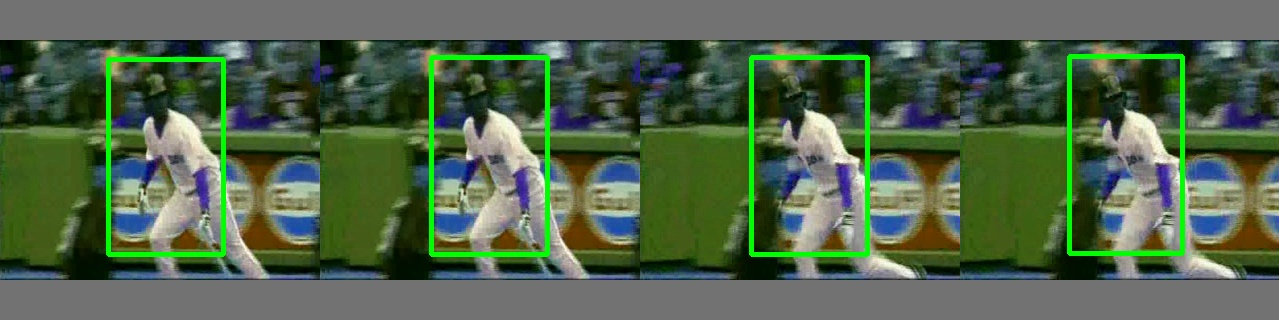
\includegraphics[width= 0.8\textwidth, height=0.1\textheight]{proposals0_half}
    \caption{}
    \label{fig:proposals0}
  \end{subfigure}

  \begin{subfigure}{1\textwidth}
    \centering
    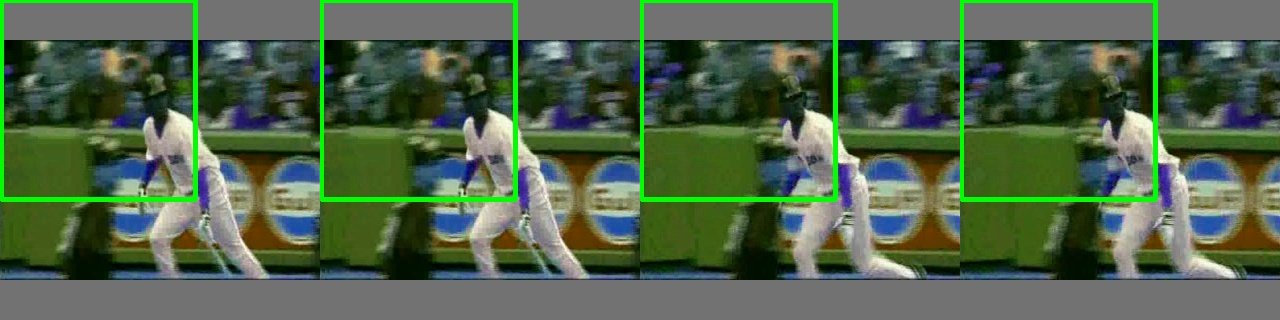
\includegraphics[width= 0.8\textwidth, height=0.1\textheight]{proposals1_half}
    \caption{}
    \label{fig:proposals1}
  \end{subfigure}

  \begin{subfigure}{1\textwidth}
    \centering
    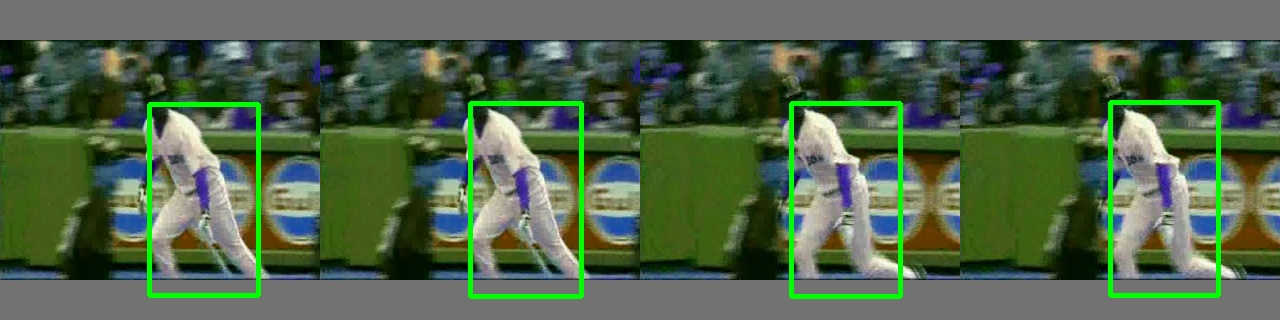
\includegraphics[width= 0.8\textwidth, height=0.1\textheight]{proposals2_half}
    \caption{}
    \label{fig:proposals2}
  \end{subfigure}

  \begin{subfigure}{1\textwidth}
    \centering
    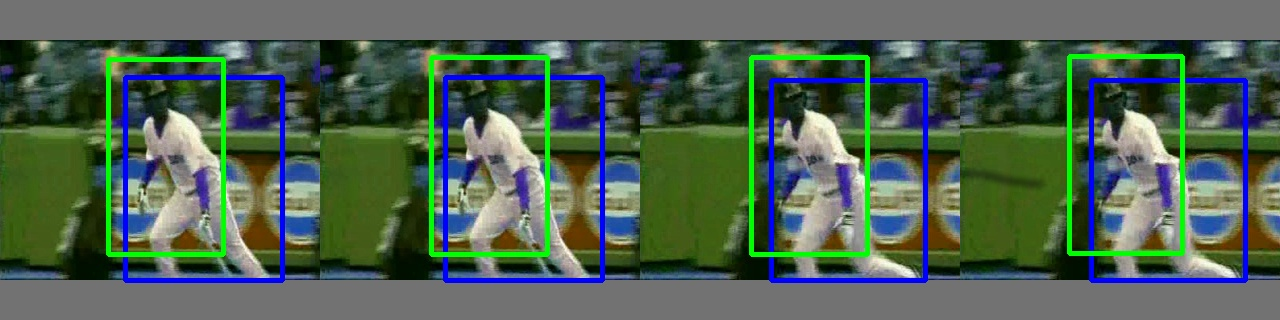
\includegraphics[width= 0.8\textwidth, height=0.1\textheight]{proposal_gt}
    \caption{}
    \label{fig:proposals_gt0}
  \end{subfigure}

  \begin{subfigure}{1\textwidth}
    \centering
    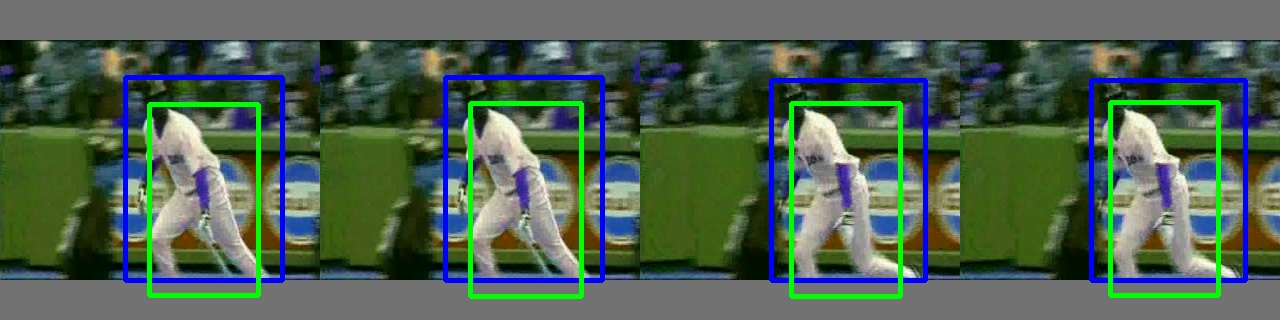
\includegraphics[width= 0.8\textwidth, height=0.1\textheight]{proposal_gt1}
    \caption{}
    \label{fig:proposals_gt1}
  \end{subfigure}
  \centering
  % \caption{(\protect\subref{fig:proposals0}),(\protect\subref{fig:proposals1}),(\protect\subref{fig:proposals2})
  %   present 3 ToIs while (\protect\subref{fig:proposals_gt0}),(\protect\subref{fig:proposals_gt1})
  %   present first 2 proposals with their corresponding grouthtruth ToI}
  \caption{ Visualization of Tois including grouthtruth action tubes, too }


  \label{fig:proposals}
\end{figure}

Our goal is  the bounding boxes to overlap with the actor precisely. According to Figure \ref{fig:proposals}, all of three proposed actions tubes
presented in Figures \ref{fig:proposals0}, \ref{fig:proposals1} and \ref{fig:proposals2} overlap with the actor to some degree.
However, by looking, it is clear that ToI, presented in Figure \ref{fig:proposals1}, doesn't overlap very well like those appearing at Figures \ref{fig:proposals0} and \ref{fig:proposals2}
Intuitively, comparing proposals from \ref{fig:proposals0} and \ref{fig:proposals2}, we think that \ref{fig:proposals0} overlaps better than \ref{fig:proposals2}.

However, as shown in Figures \ref{fig:proposals_gt0} and \ref{fig:proposals_gt1}, the second ToI better overlaps with the groundtruth. It is clear that even though
the first proposal overlaps very well with the upper body of the actor, it fails to capture the left leg, which may be a crucial factor for determining the class of the
action. The ToI shown in Figure \ref{fig:proposals_gt1} manages to capture most of the actor's body, excluding only the head, which usually doesn't move a lot
during an action. Although, judging intuitively, we would choose the first ToI, in reality, the second one is more preferable.

% \end{document}


% \documentclass{report}

% \usepackage{subcaption} % package for subfigures
% \usepackage{hyperref}  % package for linking figures etc
% \usepackage{enumitem}  % package for description with bullets
% \usepackage{graphicx}  % package for importing images
% \usepackage{mathtools} % package for math equation
% \usepackage{mathrsfs}  % package for math font
% \usepackage{indentfirst} % package for getting ident after section or paragraph
% \usepackage{multirow}  % package for tables, multirow
% \usepackage{longtable} % package for multi pages tables


% \usepackage[export]{adjustbox}
% % \usepackage{amsmath}

% \setlength{\parindent}{2em} % how much indent to use when we start a paragraph

% \graphicspath{ {./theory/figures/} }       % path for images

% \begin{document}

\chapter{Connecting Tubes}
\section{Introduction}
In the previous chapter, we described methods for generating candidate action tubes given a small video segment lasting 8 or 16 frames. However, actual videos
and actual human actions, in the  wild, last more than 16 frames most of the times. Current networks are unable to process a whole video at once, in order to generate action tubes
due to memory and computing power issues.  As mentioned in chapter 2, a lot action localization approaches deal with this situation by giving a video either
propose candidate areas in the frame-level and then they connect these in order to generate action tube proposal either, separate it into video segments,
proposing  sequences of bounding boxes for each video segment and then link them in order to generate action proposals. Both aforementioned techniques make
the suitable choice of linking method an important factor for the performance of the network. That's because, even though frame-level or video segment-level proposals
might be very good, if the proposed connection algorithm doesn't work well, final action tube proposals won't be efficient, so the final model will never
be able to achieve high classification performance. In other words, if connecting algorithm doesn't generate action proposals with great recall and MABO performance,
the model's classifier won't be able to perform suitable classification, because probably it would be given action tubes without any context.
In this chapter, we present 3 different approaches used for linking proposed ToIs generated from TPN in the previous chapter.

\section{First approach: combine overlap and actioness}
Our algorithm is inspired by \cite{DBLP:journals/corr/HouCS17}, which calculates all possible sequences of ToIs. In order find the best candidate action tubes,
it uses a score, which tells us how likely a sequence of TOIs is  to contain an action. This score is a combination of 2 metrics:
\begin{description}
\item[ Actioness,  ] which is the TOI's possibility to contain an action. This score is produced by TPN's scoring layers.
\item [ TOIs' overlapping, ] which is the IoU of the last bounding boxes of the first TOI and the first frames of the second TOI.
\end{description}

The above scoring policy can be described by the following formula:
\[ S = \frac{1}{m} \sum_ {i=1}^{m} Actioness_i + \frac{1}{m-1} \sum_{j=1}^{m-1} Overlap_{j,j+1} \]

For every possible combination of TOIs we calculate their score as show in figure \ref{fig:connection_algo}.

\begin{figure}[h]
  \centering
  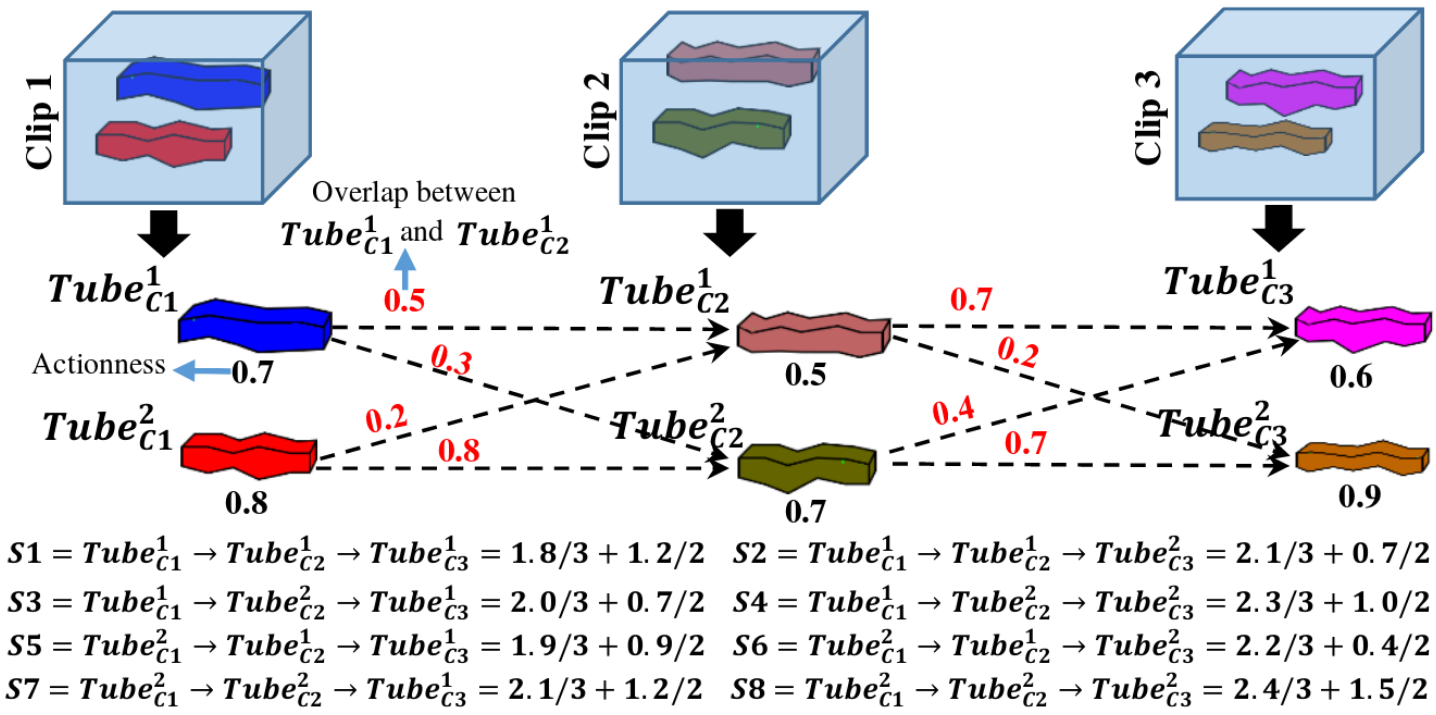
\includegraphics[scale=0.225]{connection_algo}
  \caption{An example of calculating connection score for 3 random TOIs taken from \cite{DBLP:journals/corr/HouCS17}}
  \label{fig:connection_algo}
\end{figure}

The above approach, however, needs too much memory for all needed calculations, so a memory usage  problem is
appeared. The reason is, for every new video segment, we propose \textit{k TOIs} (16 during training and 150 during validation).
As a result, for a small video separated into  \textbf{10 segments}, we need to calculate 
\textbf{  150\textsuperscript{10} scores} during validation stage. This causes our system to overload and it takes too much time to process
just one video. \par

In order to deal with this problem, we create a greedy algorithm in order to find the candidates tubes. Intuitively, this algorithm after
getting  a new video segment, keeps tubes with a score higher than a threshold, and deletes the rest. So, we don't need to calculate combinations with a
very low score. We wrote code for calculating tubes' scores in CUDA language, which has the ability to
parallel process the same code using different data. Our algorithm is described below:

\begin{enumerate}
\item Firstly,  initialize empty lists for the final tubes, final tubes' duration, their scores, active tubes, their corresponding duration,
  active tubes' overlapping sum and actioness sum where:
  \begin{itemize}
  \item Final tubes list contains all tubes which are the most likely to contain an action, and their score list contains their
    corresponding scores. We refer to each tube by its index, which is related a tensor, in which we saved all the ToIs proposed
    from TPN for each video segment.
  \item Active tubes list contains all tubes that will be matched with the new TOIs. Their overlapping sum list and actioness sum list
    contain their sums in order to avoid calculating then for each loop. 
  \end{itemize}
Also, we initialize  connection threshold equal to 0.5 .
\item For the first video segment, we add all the TOIs to both active tubes and final tubes. Their scores are only their actioness because
  there are no tubes for calculating their overlapping score. So, we set their overlaping sum equal to 0.
\item For each next video, after getting the proposed ToIs, firstly we calculate their overlapping score with each active tube. Then, we
  empty active tubes, active tubes' duration, overlapping sum and actioness score lists.  For each new tube that has a score higher than the
  connection threshold,  we add both to final tubes and to active tubes and their corresponding lists, and we increase their duration.
\item If the number of active tubes is higher than a threshold, we set connection threshold equal to the score of
  the 100th higher score. On top of that, we update the final tubes list, removing all tubes that have score lower than the threshold.
\item After that, we add in active tubes, the current video segment's proposed TOIs, alongside with their actioness scores in the  actioness sum list and
  zero values in corresponding positions in the overlaps sum list (such as in the 1st step).
\item We repeat the previous 3 steps until there is no video segment left.
\item Finally, as we mentioned before, we have a list which contains the indexes of the saved tubes. So, we modify them in order to have
  the corresponding bounding boxes. However, 2 succeeding ToIs do not, always, have exactly the same bounding boxes in the frames that overlap. For example,
  ToIs from the $1^{st}$ video segment start from frame 1 to frame 16. If we have video step equal to 8, these ToIs overlap temporally
  with the ToIs from the  succeeding video segment in frames 8-16. In those frames, in final tube, we choose the area that contains both bounding boxes which is
  denoted as $(min(x_1,x'_1), min(y_1,y'_1), max(x_2,x'_2), max(y_2,y'_2))$ for bounding boxes $(x_1,y_1,x_2,y_2)$ and $(x'_1,y'_1,x'_2,y'_2)$.
\end{enumerate}
% We implement this algorithm using CUDA language for counting the scores. In \cite{DBLP:journals/corr/HouCS17}, they use temporal \textit{stride = sample duration} during testing. We want 
\subsection{JHMDB Dataset}

In order to validate our algorithm, we firstly experiment in JHMDB dataset's videos in order to define the best overlapping policy and
the video overlapping step. Again, we use recall as evaluation metric. A groundtruth action tube is considered to be found, as well as positive,
if there is at least 1 video tube which overlaps with it over a predefined threshold, otherwise it .  These thresholds are again 0.5, 0.4 and 0.3.
We set TPN to return 30 ToIs per video segment.
We chose to update threshold when active tubes are more than 500 and to keep the first 100 tubes as active. We did so, because, a big part of the
code is performing in the CPU. That's because, we use lists, which are very easy to handle for adding and removing elements. So, if we use bigger update
limits, it takes much more time to process them.

\paragraph{Sample duration equal to 16 frames} At first we use as sample duration = 16 and video step = 8. As overlapping frames we count frames
\textit{(8...15)} so we have \#8 frames. Also, we use only \#4 frames with combinations \textit{(8...11), (10...13) and (12...15)} and 
\#2 frames with combinations \textit{(8,9), (10,11), (12,13), and (14,15)}. The results are shown in Table \ref{table:step8_16} (in bold are
the frames with which we calculate the overlap score).

\begin{center}
\begin{longtable}{||c||c c c||}

  \hline
  \multirow{2}{5em}{combination} & {} &overlap thresh & {} \\
                                    &  0.5  &  0.4 &  0.3 \\         
  \hline  \hline
  0,1,...,\textbf{\{8,...,15\}}               & {} & {} & {} \\
  \textbf{\{8,9,...,15\}},16,...,23           & 0.3172 & 0.4142 & 0.6418 \\
  \hline     \hline                          


  0,1,...,\textbf{\{8,...,11,\}}...,14,15     & {} & {} & {} \\
  \textbf{\{8,...,11\}},12,...,22,23          & 0.3172 & 0.4142& 0.6381 \\
  \hline
  0,1,...,\textbf{\{10,...,13,\}}14,15,       & {} & {} & {} \\
  8,9,\textbf{\{10,...,13\}},14,...,22,23     & 0.3209 &0.4179   & 0.6418 \\
  \hline
  0,1,...,\textbf{\{12,...,15,\}}             & {} & {} & {} \\
  8,9,...,\textbf{\{12,...,15\}},16,...,23,   & 0.3284 & 0.4216 & 0.6381 \\
  \hline     \hline                          

  0,1,...,\textbf{\{8,...,11,\}},...,14,15,   & {} & {} & {} \\
  \textbf{\{8,9,...,11,\}}12,...,22,23        & 0.3172   & 0.4142& 0.6381 \\
  \hline
  0,1,...,\textbf{\{10,...,13,\}}14,15,       & {} & {} & {} \\
  \textbf{\{10,...,13\}},14,...,22,23         & 0.3209 &0.4179   & 0.6418 \\
  \hline
  0,1,...,\textbf{\{12,...,15\}}              & {} & {} & {} \\
  8,9,...,\textbf{\{12,...,15\}},16,...       & 0.3284 & 0.4216 & 0.6381 \\
  \hline \hline
  
  0,1,...,\textbf{\{8,9,\}},10,...,14,15,     & {} & {} & {} \\
  \textbf{\{8,9,\}}10,11,...,22,23            & 0.3134   & 0.4104 & 0.6381 \\
  \hline
  0,1,...,\textbf{\{10,11,\}},12,...,14,15,   & {} & {} & {} \\
  8,9,\textbf{\{10,11,\}}12,...,22,23         & 0.3209   & 0.4216 & 0.6418 \\
  \hline
  0,1,...,\textbf{\{12,13,\}},14,15,          & {} & {} & {} \\
  8,9,...,\textbf{\{12,13,\}}14,...,22,23     & 0.3246   & 0.4179 & 0.6418 \\
  \hline
  0,1,...,13,\textbf{\{14,15,\}}              & {} & {} & {} \\
  8,9,...,\textbf{\{14,15,\}}16,...,22,23     & 0.3321   & 0.4216 & 0.6306 \\
  \hline \hline
  \caption{Recall results for step = 8}
  \label{table:step8_16}
\end{longtable} 
\end{center}

As we can from the above table, generally we get very bad performance and we got the best performance when we calculate the overlap between only 2 frames (either \textit{14,15} or \textit{12,13}).
So, we thought that we should increase the video step because, probably, the connection algorithm is too strict into big movement variations during  the video. As a result, we set video step = 12 which
means that we have only 4 frames overlap. In this case,  for \#4 frames, we only have the combination \textit{(12...15)}, for \#2 frames we have \textit{(12,13), (13,14) and (14,15)} as shown in
Table \ref{table:step12_16}.

\begin{center}
\begin{longtable}{||c||c c c||}

  \hline
  \multirow{2}{5em}{combination} & {} &overlap thresh & {} \\
                                    &  0.5  &  0.4 &  0.3 \\         
  \hline  \hline
  0,1,...,11,\textbf{\{12,...,15\}}           & {} & {} & {} \\
  \textbf{\{12,13,...,15\}},16,...,26,27         & 0.3769 & 0.4627 & 0.6828 \\
  \hline     \hline                          

  0,1,...,\textbf{\{12,13,\}},14,15,          & {} & {} & {} \\
  \textbf{\{12,13,\}}14,15,...,26,27          & 0.3694   & 0.4627 & 0.6903 \\
  \hline                          
  0,1,...,12\textbf{\{13,14,\}},15,           & {} & {} & {} \\
  12,\textbf{\{13,14,\}}15,...,26,27          & 0.3843   & 0.4627 & 0.6828 \\
  \hline                          
  0,1,...,12,13\textbf{\{14,15,\}}            & {} & {} & {} \\
  12,13,\textbf{\{14,15,\}}16,...,26,27       & 0.3694   & 0.459 & 0.6828 \\
  \hline     \hline                          

  \caption{Recall results for step = 12}
  \label{table:step12_16}
\end{longtable} 
\end{center}

As we can see, recall performance is increased so that means that our assumption was correct. So again, we increase video step into 14, 15 and 16 frames
and recall score is shown in Table \ref{table:step14_16}
\begin{center}
\begin{longtable}{||c||c c c||}

  \hline
  \multirow{2}{5em}{combination} & {} &overlap thresh & {} \\
                                    &  0.5  &  0.4 &  0.3 \\         
  \hline  \hline
  0,1,...,13\textbf{\{14,15\}}                & {} & {} & {} \\
  \textbf{\{14,15\}},16,...,28,29                & 0.3731 & 0.5336 & 0.6493 \\
  \hline     \hline                          

  0,1,...,13,\textbf{\{14,\}}15,              & {} & {} & {} \\
  \textbf{\{14,\}}15,...,28,29                & 0.3694   & 0.5299 & 0.6455 \\
  \hline                          
  0,1,...,14,\textbf{\{15\}}                  & {} & {} & {} \\
  14,\textbf{\{15,\}}16,...,28,29             & 0.3731   & 0.5187 & 0.6381 \\
  \hline  \hline

  0,1,...,14,\textbf{\{15\}}                & {} & {} & {} \\
  \textbf{\{15\}},16,...,30                 & 0.3918 & 0.5187 & 0.6381 \\
  \hline     \hline                          
  0,1,...,14,\textbf{\{15\}}                & {} & {} & {} \\
  \textbf{\{16\}},17,...,31                 & 0.4067 & 0.7313 & 0.8731 \\
  \hline                          
  \caption{Recall results for steps = 14, 15 and 16}
  \label{table:step14_16}
\end{longtable} 
\end{center}

The results show that we get the best recall performance when we have no overlapping steps and video step = 16 = sample duration. We try to improve
more our results, using smaller duration because, as we saw from TPN recall performance, we get better results when we have sample duration = 8 or 4.

\paragraph{Sample duration equal to  8}
We wanted to confirm that we get the best results, when we have no overlapping frames and step = sample duration. So Table \ref{table:step4_8}
shows recall performance for sample duration = 8 and video step = 4 and Table \ref{table:step8_678 } for video steps = 6, 7 and 8.


\begin{center}
\begin{longtable}{||c||c c c||}

  \hline
  \multirow{2}{5em}{combination} & {} &overlap thresh & {} \\
                                    &  0.5  &  0.4 &  0.3 \\         
  \hline  \hline
  0,1,2,3,13\textbf{\{4,5,6,7\}}                & {} & {} & {} \\
  \textbf{\{4,5,6,7\}},8,9,10,11                & 0.2015   & 0.3582 & 0.5858 \\
  \hline     \hline                          

  0,1,2,3,\textbf{\{4,5,\}}6,7                  & {} & {} & {} \\
  \textbf{\{4,5,\}}6,7,8,9,10,11                & 0.1978   & 0.3582 & 0.5933 \\
  \hline                          
  0,1,2,3,4\textbf{\{5,6,\}}7                   & {} & {} & {} \\
  4,\textbf{\{5,6,\}}7,8,9,10,11                & 0.1978   & 0.3507 & 0.5821 \\
  \hline                          
  0,1,2,3,4,5\textbf{\{6,7\}}                   & {} & {} & {} \\
  4,5,\textbf{\{6,7,\}}8,9,10,11                & 0.194   & 0.3433 & 0.585 \\
  \hline                           
  \caption{Recall results for step = 4}
  \label{table:step4_8}
\end{longtable} 
\end{center}

\begin{center}
\begin{longtable}{||c||c c c||}

  \hline
  \multirow{2}{5em}{combination} & {} &overlap thresh & {} \\
                                    &   0.5  &  0.4 &  0.3 \\         
  \hline  \hline
  0,1,2,3,4,5\textbf{\{6,7\}}           & {} & {} & {} \\
  \textbf{\{6,7\}},8,9,10,11,12,13      & 0.3134  & 0.7015 & 0.8619 \\
  \hline     \hline                          

  0,1,2,3,4,5,\textbf{\{6,\}}7          & {} & {} & {} \\
  \textbf{\{6,\}}7,8,9,10,11,12,13      & 0.3209  & 0.6679 & 0.847 \\
  \hline                          
  0,1,2,3,4,5,6,\textbf{\{7\}}          & {} & {} & {} \\
  6,\textbf{\{7\}}8,9,10,11,12,13       & 0.3172  & 0.6567 & 0.8507 \\
  \hline                          
  0,1,2,3,4,5,6\textbf{\{7\}}           & {} & {} & {} \\
  \textbf{\{7,\}}8,9,10,11,12,13,14     & 0.5597  & 0.7687 & 0.903 \\
  \hline                           
  0,1,2,3,4,5,6\textbf{\{7\}}           & {} & {} & {} \\
  \textbf{\{8\}}9,10,11,12,13,14,15     & 0.653	  & 0.8396 &0.9179  \\
  \hline                           
  \caption{Recall results for steps = 6, 7 and 8}
  \label{table:step8_678 }
\end{longtable} 
\end{center}

According to Tables \ref{table:step4_8} and \ref{table:step8_678 }, it is clearly shown that, we achieve the  best results, for $step = sample duration$ and overlapping scores is calculated between the last box of the current tubes and the first box of next tubes.

\subsection{UCF dataset}
In previous steps, we tried to find the best overlap policy for our algorithm in JHMDB dataset. After that, it's time to apply our algorithm in UCF dataset using the best scoring
overlap policy. We did some modifications in the code, in order to use less memory and we moved most parts of the code to the GPU. This happened by using tensors instead of lists for scores while
most operations are, from now on, matrix operations. On top that, the last step of the algorithm, which is the modification from indices to actual action tubes is written, now, in CUDA code so
it takes place in the GPU, too. So, we are now able to increase the number of ToIs returned by TPN, the max number of active tubes before updating threshold and the max number of final
tubes. \par
The first experiments we performed were related to the number of the final tubes, our network proposes alongside with TPN's proposed
tubes' number. We experiment for cases, in which TPN proposes 30, 100 and 150 ToIs, our final network proposes 500, 2000 and 4000
candidate action tubes for sample durations equal to 8 and 16 frames.
For the sample duration equal to 8 we return 100 ToIs because, when we tried to return 150 proposed ToIs, we got OutOfMemory error.
Table \ref{table:ucf_recall} show the spatiotemporal recall and MABO performance of those approaches. Furthermore, Table \ref{table:ucf_temp_recall } show their temporal recall and MABO performance. We are interested in temporal performance, because UCF consists of
untrimmed videos, unlike JHMDB which has only trimmed videos. So, we want to know how well our network is able to propose action tubes that
overlap temporally with the groundtruth action tubes over a ``big'' threshold. For temporal localization, we don't use 0.5, 0.4 and 0.3
overlapping threshold, but instead, we use 0.9, 0.8 and 0.7, because it is very important our network to be able to propose tubes that
 contain an action, at least from the temporal perspective. In order to calculate the temporal overlap, we use IoU for 1 dimension as described before.

\begin{center}
\begin{longtable}{||c | c | c ||c c c | c|}

  \hline
  \multirow{2}{*}{combination} & \multirow{2}{2.5em}{TPN tubes} & \multirow{2}{2.5em}{Final tubes} &  \multicolumn{3}{}{overlap thresh} & \multirow{2}{*}{MABO} \\
  {} & {} & {} &  0.5 &  0.4 & 0.3 & {}\\         
  \hline
  
  \multirow{6}{7em}{0,1,...,6,\textbf{\{7,\}}
  \textbf{\{8,\}}9,...,14,15 }  & \multirow{3}{*}{30} & 500   & 0.2829  & 0.4395 & 0.5817  & 0.3501 \\
  \cline{3-7}
  {} &  {}   & 2000   & 0.3567  & 0.4996 & 0.6289 & 0.3815\\
  \cline{3-7}
  {} &  {}   & 4000   & 0.3749  & 0.5316 & 0.6487 & 0.3934 \\
  \cline{2-7}
  {} &  \multirow{3}{*}{100}   & 500   & 0.2966  & 0.451 & 0.5947 & 0.356 \\
  \cline{3-7}
  {} &  {}   & 2000   & 0.3757  & 0.5163 & 0.6471 & 0.3902 \\
  \cline{3-7}
  {} &  {}   & 4000  & 0.3977  & 0.5506 & 0.6624 & 0.4029 \\
  \hline                                    
  \multirow{6}{7em}{0,1,...,14,\textbf{\{15,\}}
  \textbf{\{16,\}}17,18,...,23 }  & \multirow{3}{*}{30} & 500   & 0.362  & 0.5042 & 0.6243 & 0.3866 \\
  \cline{3-7}
  {} &  {}   & 2000   & 0.416  & 0.5468 & 0.6631 & 0.4108  \\
  \cline{3-7}
  {} &  {}   & 4000   & 0.4281  & 0.5589  & 0.6779 & 0.4182 \\
  \cline{2-7}
  {} &  \multirow{3}{*}{150}   & 500 & 0.3589  & 0.4981 & 0.6198 & 0.3845 \\
  \cline{3-7}
  {} &  {}   & 2000   & 0.4129  & 0.5392  & 0.6563 & 0.4085 \\
  \cline{3-7}
  {} &  {}   & 4000   & 0.4266  & 0.5521 & 0.6722 & 0.4162\\
  \hline                                    

  \caption{Recall results for UCF dataset}
  \label{table:ucf_recall}
\end{longtable} 
\end{center}

\begin{center}
\begin{longtable}{||c | c | c ||c c c| c|}

% \begin{table}
%   \centering
%   \setlength{\tabcolsep}{4pt}
%   \begin{tabular}{||c | c | c ||c c c| c|}

  \hline
  \multirow{2}{*}{combination} & \multirow{2}{2.5em}{TPN tubes} & \multirow{2}{2.5em}{Final tubes} &  {} &overlap thresh & {} & \multirow{2}{*}{MABO} \\
  {} & {} & {} &  0.9 &  0.8 & 0.7 & {}\\         
  \hline
  
  
  \multirow{6}{7em}{0,1,...,6,\textbf{\{7,\}}
  \textbf{\{8,\}}9,...,15 }  & \multirow{3}{*}{30} & 500   & 0.4464  & 0.581 & 0.6844  & 0.7787 \\
  \cline{3-7}
  {} &  {}   & 2000   & 0.635  & 0.7665 & 0.8403 & 0.8693 \\
  \cline{3-7}
  {} &  {}   & 4000   & 0.7034  & 0.8228 & 0.8875 & 0.8973 \\
  \cline{2-7}
  {} &  \multirow{3}{*}{100}   & 500   & 0.454 & 0.5924 & 0.692 & 0.783 \\
  \cline{3-7}
  {} &  {}   & 2000   & 0.651 & 0.7696 & 0.8441 &0.8734 \\
  \cline{3-7}
  {} &  {}   & 4000   & 0.7209 &0.8312 & 0.8913 & 0.9026 \\

  \hline                                    
  \multirow{6}{7em}{0,1,...,14,\textbf{\{15,\}}
  \textbf{\{16,\}}17,18,...,23 }  & \multirow{3}{*}{30} & 500   & 0.6844 &0.8327 & 0.9027 & 0.8992 \\
  \cline{3-7}
                                    {} &  {}   & 2000   & 0.7475 & 0.8684 & 0.9217 & 0.9175 \\
  \cline{3-7}
                                    {} &  {}   & 4000   & 0.7567  & 0.8745  & 0.9255 & 0.9211 \\
  \cline{2-7}
                                    {} &  \multirow{3}{*}{150}   & 500   & 0.7498 &0.8707 &0.9171 & 0.9125 \\
  \cline{3-7}
                                    {} &  {}   & 2000   & 0.8243 & 0.911 & 0.9392 & 0.9342\\
  \cline{3-7}
                                    {} &  {}   & 4000   &  0.8403  & 0.9179 & 0.9437 & 0.9389\\
  \hline                                    
  % \end{tabular}
  \caption{Temporal Recall results for UCF dataset}
  \label{table:ucf_temp_recall }
% \end{table}
\end{longtable} 
\end{center}

According to Table \ref{table:ucf_recall}, we achieve better recall and MABO performance when we set sample duration equal to 16.
In all cases,  recall performance of simulations with sample duration equal to  16 outweight the corresponding with 8, with the difference
varying from 2\% to 8\%. In addition, we get best recall and MABO performance when our system proposes 4000 tubes. As we can see,
the ratio of good proposals increases about 5\%-7\% when we change number of proposed tubes from 500 to 2000. This ratio increases more
when we double returned action tubes, from 2000 to 4000. However, this increase is only about 1\%-2\%, which make us rethink if this increase
is worth to be performed. That's because, this modification increases memory usage, because of 4000 proposed action tubes, instead of
2000. Finally, Table \ref{table:ucf_recall} shows that, for sample duration = 8, changing the number of ToIs produced by TPN, slightly
helps our network to achieve better results. This contribution is measured about 1\%-2\%.
On the contrary, when we set sample duration equal to 16, it slightly reduces network's performance. Taking all the aforementioned
results into account, we think that the most suitable choices for connection approaches are, for the sample duration equal to 8, the one in
which TPN returns 100 ToIs and our network proposes 4000 action tubes, and for the sample duration equal to 16, the one in which,
TPN returns 30 ToIs and the network 4000 action tubes. \par
Additionally, Table \ref{table:ucf_temp_recall } shows some interesting facts, too. At first, it confirms that increasing the number of proposed
action tubes, from 500 to 4000, increases recall and MABO performance. Also, we get better results when network has 16 frames as sample
duration, too. However, unlike Table \ref{table:ucf_recall}, Table \ref{table:ucf_temp_recall } shows that when we increase TPN's number
of proposed ToIs, it increases performances for both sample durations. For sample duration equal to 8, this increase results in improving
recall performances by 2\% and MABO performance by 1\% like spatiotemporal recall and MABO. For the sample duration equal to 16, recall
performance is increasing by about 8\% and MABO by 1\%-2\%.  \par
Taking both tables into consideration, we think that the best approach is TPN returning 30 proposed ToIs, network returning 4000 proposed
action tubes and sample duration equals with 16. We didn't choose TPN returning 150 proposed ToIs because, based on MABO performances,
they different only by 1\%, difference which is insignificant.


\subsubsection{Adding NMS algorithm}

Previous section describes the performances of network's proposals for variations in the number of  TPN's  returned ToIs, number of returned
proposed action tubes and sample duration. For each situation, we choose the k-best scoring action tubes, without taking into account
any relation between these action tubes, like their spatiotemporal overlap. So, like TPN's approach, we thought that we should apply
nms algorithm before choosing k-best scoring tubes, in order to further improve  spatiotemporal and temporal, recall and MABO  performance.
We experiment using again two sample durations, 16 and 8 frames per video segment, number or TPN's returning tubes equal to 30 and the
number of final picked action tubes equal to 4000. NMS algorithm uses a threshold in order to choose if 2 action tubes overlap enough. We
experiment setting this threshold equal to 0.7 and 0.8 and  the results are shown in Table \ref{table:ucf_nms_recall} for Spatiotemporal
performance and at Table \ref{table:ucf_nms_temp_recall} for temporal performance.

\begin{center}
  \setlength{\tabcolsep}{2pt}
\begin{longtable}{||c | c | c | c c c| c|}

  \hline
  \multirow{2}{*}{combination} & \multirow{2}{2.5em}{NMS thresh} & \multirow{2}{3.5em}{PreNMS tubes} &  {} &overlap thresh & {} & \multirow{2}{*}{MABO} \\
  {} & {} & {} &  0.9 &  0.8 & 0.7 & {}\\         
  \hline
  \multirow{3}{7em}{0,1,...,6,\textbf{\{7,\}}
  \textbf{\{8,\}}9,...,15 }  & 0.7 &\multirow{3}{*}{20000}  & 0.346 & 0.5202 & 0.657 & 0.3824685269 \\
  \cline{2-2} \cline{4-7} 
  {} &  0.8   & {}   & 0.3643 & 0.5392 & 0.6578 & 0.3904727407 \\
  \cline{2-2} \cline{4-7} 
  {} &  0.9   & {}   & 0.397  & 0.5574 & 0.6677 & 0.4031543642 \\
  \hline                                    
  \multirow{3}{7em}{0,1,...,14,\textbf{\{15,\}}
  \textbf{\{16,\}}17,...,23 }  & 0.7 & \multirow{3}{*}{20000}   & 0.3939 & 0.5559  & 0.6882 & 0.404689056 \\
  \cline{2-2} \cline{4-7} 
                                    {} &  0.8   & {}   & 0.4259 & 0.5764 & 0.6981 & 0.419487652 \\
  \cline{2-2} \cline{4-7} 
                                    {} &  0.9   & {}   & 0.4494 & 0.5856 & 0.7019 & 0.4302611039 \\

  \hline                                    

  \caption{Spatiotemporal Recall results for UCF dataset}
  \label{table:ucf_nms_recall}
\end{longtable} 
\end{center}

\begin{center}
  \setlength{\tabcolsep}{2.2pt}
\begin{longtable}{||c | c | c | c c c| c|}

  \hline
  \multirow{2}{*}{combination} & \multirow{2}{2.5em}{NMS thresh} & \multirow{2}{3.5em}{PreNMS tubes} &  {} &overlap thresh & {} & \multirow{2}{*}{MABO} \\
  {} & {} & {} &  0.9 &  0.8 & 0.7 & {}\\         
  \hline
  \multirow{3}{7em}{0,1,...,6,\textbf{\{7,\}}
  \textbf{\{8,\}}9,...,15 }  & 0.7 &\multirow{3}{*}{20000}  & 0.6281 & 0.8251 & 0.9027 & 0.8885141223  \\
  \cline{2-2} \cline{4-7} 
  {} &  0.8   & {}   & 0.7369 & 0.8616 & 0.9148 & 0.9106069806 \\
  \cline{2-2} \cline{4-7} 
  {} &  0.9   & {}   &  0.7787 & 0.8753 & 0.9209 & 0.9212593589 \\
  \hline                                    
  \multirow{3}{7em}{0,1,...,14,\textbf{\{15,\}}
  \textbf{\{16,\}}17,...,23 }  & 0.7 & \multirow{3}{*}{20000}   & 0.7452 & 0.8920 & 0.9361 & 0.920331595 \\
  \cline{2-2} \cline{4-7} 
  {} &  0.8   & {}   & 0.8160 & 0.9278 & 0.9506 & 0.93612757 \\
  \cline{2-2} \cline{4-7} 
  {} &  0.9   & {}   & 0.854 & 0.9346 & 0.9529 & 0.9434986107 \\
  \hline                                    

  \caption{Temporal Recall results for UCF dataset}
  \label{table:ucf_nms_temp_recall}
\end{longtable} 
\end{center}

Comparing Table \ref{table:ucf_nms_recall} with Table \ref{table:ucf_recall},  we notice that NMS algorithm improves recall and MABO
performance when NMS threshold is equal to 0.9. When we set it equal to 0.7 or 0.8, we get worse results. This happens, probably, because
nms algorithm removes some good proposals. Comparing these results with results presented at Tables \ref{table:ucf_recall} and \ref{table:ucf_temp_recall } it becomes clear that using NMS algorithm is very useful. That's because, even though we get the same number of proposed action tubes,
these tubes are not very close spatiotemporally, so this makes proposed action tubes more likely to contain actual foreground action tubes.

\subsubsection{Stop updating threshold}

In previous approaches, scoring threshold was updated each time our algorithm gathered a significant number of ``active'' tubes in order not
to add action tubes with score below this score. However, after serious consideration, we came to the conclusion that sometimes, the updated
threshold leads to not detecting action tubes that start after some frames. That's because, until then, linking threshold may be too big that
won't let new action tubes to be created. So, we came with the modification of not updating linking threshold, but just filtering proposed
tubes, by keeping k-best scoring each time their number is bigger that the a specific number. The rest algorithm remains the same. Tables
\ref{table:ucf_nms_noup_recall} and \ref{table:ucf_nms_noup_temp_recall} show spatiotemporal and temporal, recall and MABO performance respectively.
We experiment for cases in which either we don't use the  NMS algorithm at all, either we set overlap threshold equal to 0.7 and 0.9 as shown
below.

\begin{center}
  \setlength{\tabcolsep}{2pt}
\begin{longtable}{||c | c | c | c c c| c|}

  \hline
  \multirow{2}{*}{combination} & \multirow{2}{2.5em}{NMS thresh} & \multirow{2}{3.5em}{PreNMS tubes} &  {} &overlap thresh & {} & \multirow{2}{*}{MABO} \\
  {} & {} & {} &  0.9 &  0.8 & 0.7 & {}\\         
  \hline
  \multirow{3}{7em}{0,1,...,6,\textbf{\{7,\}}
  \textbf{\{8,\}}9,...,15 }   &   \multicolumn{2}{|c|}{-}     &  0.3779 & 0.5316 & 0.6471 & 0.393082961 \\
  \cline{2-7}
  {} & 0.7 &\multirow{2}{*}{20000}  & 0.3483  & 0.5194 & 0.6471 & 0.3783524086 \\
  \cline{2-2} \cline{4-7} 
  {} &  0.9   & {}   & 0.416 & 0.5605 & 0.6722 & 0.4074053106 \\
  \hline                                    
  \multirow{3}{7em}{0,1,...,14,\textbf{\{15,\}}
  \textbf{\{16,\}}17,...,23 }  &   \multicolumn{2}{|c|}{-} & 0.438 & 0.5635 & 0.6829 & 0.4231788 \\
  \cline{2-7}
  {} & 0.7 & \multirow{2}{*}{20000}   & 0.4525 & 0.5848 & 0.7034 & 0.429747438 \\
  \cline{2-2} \cline{4-7} 
  {} &  0.9   & {}   & 0.3802 & 0.5133 & 0.6068 & 0.3862278851848662 \\

  \hline                                    

  \caption{Spatiotemporal Recall results for UCF dataset}
  \label{table:ucf_nms_noup_recall}
\end{longtable} 
\end{center}

\begin{center}
  \setlength{\tabcolsep}{2.2pt}
\begin{longtable}{||c | c | c | c c c| c|}

  \hline
  \multirow{2}{*}{combination} & \multirow{2}{2.5em}{NMS thresh} & \multirow{2}{3.5em}{PreNMS tubes} &  {} &overlap thresh & {} & \multirow{2}{*}{MABO} \\
  {} & {} & {} &  0.9 &  0.8 & 0.7 & {}\\         
  \hline

  \multirow{3}{7em}{0,1,...,6,\textbf{\{7,\}}
    \textbf{\{8,\}}9,...,15 }  &   -   & -    & 0.7087 & 0.8281 & 0.8913 & 0.899210587 \\
  \cline{2-7} 
  {} & 0.7 &\multirow{2}{*}{20000}  & 0.6586 & 0.854 & 0.9278 & 0.903373468 \\
  \cline{2-2} \cline{4-7} 
  {} &  0.9   & {}   &  0.8137 & 0.8973 & 0.9361 & 0.9333068498 \\
  \hline                                    
  \multirow{3}{7em}{0,1,...,14,\textbf{\{15,\}}
  \textbf{\{16,\}}17,...,23 }  &   \multicolumn{2}{|c|}{-} & 0.8327 & 0.9156 &0.9399 & 0.940143272 \\
  \cline{2-7}
  {} & 0.7 & \multirow{2}{*}{20000}& 0.8646 & 0.9369 & 0.9567 & 0.946701832 \\
  \cline{2-2} \cline{4-7} 
  {} &  0.9   & {}   & 0.6183 & 0.7696 & 0.8388 & 0.8628507037919737 \\
  \hline                                    

  \caption{Temporal Recall results for UCF dataset}
  \label{table:ucf_nms_noup_temp_recall}
\end{longtable} 
\end{center}

Comparing recall and MABO performances shown at Table \ref{table:ucf_nms_noup_recall} with those included in Tables \ref{table:ucf_nms_recall}
and \ref{table:ucf_recall}, we deduce that for the sample duration equal to 8, stopping updating linking threshold results in worse performance
when we set nms threshold equal to 0.7, but it achieves the best performances  when setting NMS threshold equal to 0.9 . Furthermore, for sample duration
equal to 16, we get, now,  best performance performance when we set nms threshold equal to 0.7 and worse performance for nms threshold equal to 0.9 .

\subsubsection{Soft-nms instead of nms}

After widely experiment using NMS algorithm, we thought that we should try to use Soft-NMS algorithm, introduced by \cite{DBLP:journals/corr/BodlaSCD17} and described in chapter 2. We implement our own soft-nms algorithm modifying it in order to calculate spatiotemporal overlapping
scores, and not just spatial, like the one implemented by \cite{DBLP:journals/corr/BodlaSCD17}. As mentioned before, instead of removing action tubes, Soft-NMS algorithm just reduces their score for those which overlap over a predefined threshol. We experiment for the sample duration
equal to 8 and thresholds equal to 0.7 and 0.9, because, our implementation ran out of memory for sample duration equal to 16.
Recall and MABO performance are presented in Tables \ref{table:ucf_softnms_recall} and \ref{table:ucf_softnms_temp_recall}

\begin{center}
  \setlength{\tabcolsep}{2pt}
\begin{longtable}{||c | c | c | c c c| c|}

  \hline
  \multirow{2}{*}{combination} & \multirow{2}{2.5em}{NMS thresh} & \multirow{2}{3.5em}{PreNMS tubes} &  {} &overlap thresh & {} & \multirow{2}{*}{MABO} \\
  {} & {} & {} &  0.9 &  0.8 & 0.7 & {}\\         
  \hline
  \multirow{2}{7em}{0,1,...,6,\textbf{\{7,\}}
  \textbf{\{8,\}}9,...,15 }  & 0.7 &\multirow{2}{*}{20000}  & 0.3916 & 0.5384 & 0.6464 & 0.3964639 \\
  \cline{2-2} \cline{4-7} 
  {} &  0.9   & {}   & 0.4023 & 0.5430 & 0.6502 & 0.398845313 \\
  \hline                                    

  \caption{Spatiotemporal Recall results for UCF dataset using Soft-NMS}
  \label{table:ucf_softnms_recall}
\end{longtable} 
\end{center}

\begin{center}
  \setlength{\tabcolsep}{2.2pt}
\begin{longtable}{||c | c | c | c c c| c|}

  \hline
  \multirow{2}{*}{combination} & \multirow{2}{2.5em}{NMS thresh} & \multirow{2}{3.5em}{PreNMS tubes} &  {} &overlap thresh & {} & \multirow{2}{*}{MABO} \\
  {} & {} & {} &  0.9 &  0.8 & 0.7 & {}\\         
  \hline

  \multirow{2}{7em}{0,1,...,6,\textbf{\{7,\}}
    \textbf{\{8,\}}9,...,15 }  & 0.7 &\multirow{2}{*}{20000}  & 0.7521 & 0.8586 & 0.9110 & 0.915746097  \\
  \cline{2-2} \cline{4-7} 
  {} &  0.9   & {}   & 0.7741 & 0.8768 & 0.9255 & 0.922677864 \\
  \hline                                    

  \caption{Temporal Recall results for UCF dataset using SoftNMS}
  \label{table:ucf_softnms_temp_recall}
\end{longtable} 
\end{center}

Taking results at Tables \ref{table:ucf_softnms_recall} and \ref{table:ucf_softnms_temp_recall} into consideration, alongside with those
at Tables \ref{table:ucf_nms_noup_recall} and \ref{table:ucf_nms_noup_temp_recall} for sample duration equal to 8, we notice that
using softNMS results in slightly better results. This happens when we set overlapping threshold equal to 0.9, otherwise, for
overlapping threshold 0.7, we get worst performance. Despite the fact that softnms results in better recall and MABO performance,
our implementation is very slow, which means that for a 201-frame video, softNMS part lasts about 32 seconds on the contrary with
standard NMS algorithm without updating linking threshold, in which this part last only 2 seconds. So, we choose to use the standard NMS
algorithm without updating liking threshold as an algorithm for  removing overlapping action tubes.

\section{Second approach: use progression and progress rate}
As we saw before, our first connecting algorithm doesn't have very good recall results. So, we created another algorithm which is based on
the one proposed by \cite{DBLP:journals/corr/abs-1903-00304}. This
algorithm introduces two new metrics according to \cite{DBLP:journals/corr/abs-1903-00304}:

% TODO add more description
\begin{description}
\item[ Progression,  ] which describes the probability of a specific action being performed in the TOI. 
  We add this factor because we have noticed that actioness is tolerant to false positives. Progression is
  mainly a rescoring mechanism for each class (as mentioned in \cite{DBLP:journals/corr/abs-1903-00304})

\item [ Progress rate, ] which is defined as the progress proportion that each action class has been performed.
  
\end{description}

So, each action tube is described as a set of TOIs
\[  T = {\{ {\bf t}_i^{(k)} | {\bf t}_i^{(k)} = ( t_i^{(k)}, s_i^{(k)}, r_i^{(k)} ) \}}_{i=1:n^{(k)},k=1:K} \]
where $ t_i^{(k)} $ contains TOI's spatiotemporal information, $ s_i^{(k)} $ its confidence score and $ r_i^{(k)} $ its progress rate.

In this approach, each class is handled separately, so for the rest section, we discuss action tube generation for one class only. In order to link 2 TOIs, for
a video with N video segments, the following steps are applied:
\begin{enumerate}
\item For the first video segment (k = 1), initialize an array with the M best scoring TOIs, which will be considered as active action tubes ( AT ).
  Correspondingly, initialize an array with M progress rates  and M confidence scores.
\item For k = 2:N, execute (a) to (c) steps:
  \begin{enumerate}
  \item Calculate overlaps between $ AT^{(k)} $ and $ TOIs^{(k)}. $
  \item Connect all tubes which satisfy the following criteria:
    \begin{enumerate}
    \item $ overlap score(at_i^{(k)},t_j^{(k)})   < \theta, 
      at  \varepsilon AT^{(k)}, t \varepsilon TOIs^{(k)}  $
    \item $r(at_i^{(k)}) < r(t_j^{(k)}) $ or 
      $r(t_i^{(k)}) - r(at_i{(k)}) < \lambda $
    \end{enumerate}
    
  \item For all new tubes update confidence score and progress rate as follows:
    \begin{description}
    \item The new confidence score is the average score of all connected TOIs:
      \[  s_z^{(k+1)} = \frac {1} {n} \sum_{n=0}^{k} s_i^{(n)}\]
    \item New progress rate is the highest progress rate:
      \[r(at_z^{(k+1)} = max(r(at_i^{(k)}), r(t_j^{(k)})) \]
    \end{description}
    % \item If $ progressrate(at_i^{(k)}) < progressrate(t_i^{(k)}) $ then $ progressrate(at_i^{(k+1)}) =
  \item Keep M best scoring action tubes as active tubes and keep K best scoring action tubes for classification.
  \end{enumerate}
  
\end{enumerate}

This approach has the advantage that we don't need to perform classification again because we already know the class of
each final tube. In order to validate our results, now, we calculate the recall only from the tubes which have the same
class as the groundtruth tube. Again, we considered a groundtruth  tube as positive if there is at least one proposed  tube
that overlaps with it over the predefined threshold

\begin{center}
\begin{longtable}{||c c||c c c||}
  \hline
  \multicolumn{2}{||c||}{\textbf{combination}} &\multicolumn{3}{|c||}{\textbf{overlap thresh}}\\

  \hline
  sample dur & step &   0.5  &  0.4 &  0.3 \\
  \hline   \hline
  8 & 6 & 0.3284 & 0.5 & 0.6082  \\
  \hline
  8 & 7 & 0.209	& 0.459 & 0.6119 \\
  \hline
  8 & 8 & 0.3060 & 0.5672 & 0.6866 \\
  \hline
  16 & 8  & 0.194 & 0.4366 & 0.7164 \\
  \hline
  16 & 12 & 0.3358 & 0.5336 & 0.7537 \\
  \hline
  16 & 16 & 0.2649 & 0.4664 & 0.709 \\
  
  \hline     \hline                          

  \caption{Recall results for second approach with step = 8, 16 and their corresponding steps }
  \label{table:conn_app2}
\end{longtable} 
\end{center}

According to  Table \ref{table:conn_app2}, we get the best performance when we set sample duration equal to  16 and overlap step equal to 12.
Comparing this performance with the first approach, for both sample durations equal to 8 and 16, we notice that second approach falls short
comparing to the first one. 

\section{Third approach : use naive algorithm - only for JHMDB}

As mention in the first approach, \cite{DBLP:journals/corr/HouCS17} calculate all possible sequences of ToIs in order to the find the best
candidates. We rethought about this approach and we concluded that it could be implemented for JHMDB dataset if we reduce the number of proposed
ToIs, produced by TPN,  to 30 for each video clip. We exploited the fact that JHMDB dataset's videos are trimmed, so we do not need to look
for action tubes starting in the second video clip which saves us a lot of memory. On top of that, we modified our code
in order to be more memory efficient  writing some parts using CUDA programming language, saving a lot of processing power, too. \par
So, after computing all possible combinations starting of the first video clip and ending in the last video clip, we keep only the
\textbf{k-best scoring tubes (k = 500) }. We run experiments which have sample duration equal to 8 and 16 frames and we modify the video step each time.
For sample duration = 8, we return only 15 ToIs and for sample duration = 16, we return 30 because, if we return more, we get ``out of memory error''.
In the following table, we can see the recall results. \par  

\begin{center}
\begin{longtable}{||c c||c c c||}

  \hline
  \multicolumn{2}{||c||}{\textbf{combination}} &\multicolumn{3}{|c||}{\textbf{overlap thresh}}\\
  \hline
  sample dur & step &  0.5  &  0.4 &  0.3 \\
  \hline   \hline

  8 & 6 & 0.7873 & 0.8657 & 0.9366  \\
  \hline
  8 & 7 & 0.7836 & 0.8731 & 0.9366  \\
  \hline
  8 &  8 & 0.7910 & 0.8806 & 0.9515 \\
  \hline 

  16 & 8  & 0.7873 & 0.8843 & 0.9291 \\
  \hline
  16 & 12 & 0.7948 & 0.8881 & 0.9403 \\
  \hline
  16 & 16 & 0.7985 & 0.8918 & 0.9515 \\
  \hline \hline
  \caption{Recall results for second approach with  }
  \label{table:conn_app3}
\end{longtable} 
\end{center}

From the above table, firstly, we confirm that when video step is equal to the sample duration gives us the best recall results.
Also, we notice that when sample duration is equal to 16  frames recall gets slightly better that when sample duration is
equal to 8. However, using  16 frames per video segment sample increases the memory usage even though it reduces the number of video segments, because of the
need to process bigger videos, bigger feature maps etc. So for the classification stage we will experiment using mostly sample duration equal
with 8 frames.

\section {General comments}

\begin{figure}[h]
  % 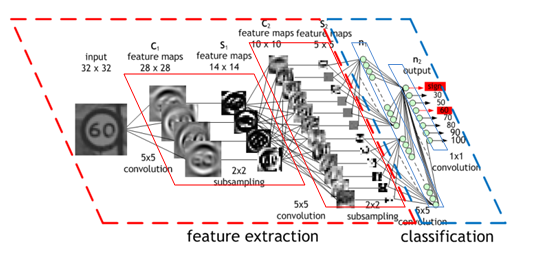
\includegraphics[scale=0.7]{convolutional_neural_network_structure} \]
  \centering
  % \includegraphics[scale=0.2]{tube_ex2_half}
  \includegraphics[width= 0.8\textwidth, height=0.45\textheight]{tube_ex2_half}
  \caption{Example of connected tubes}
  \label{fig:tube_ex}
\end{figure}

Figure \ref{fig:tube_ex} shows the example presented in chapter 3, after linking first video segment's first ToI with a ToI proposed for the second video segment. For this case, we used the third proposed method, including calculating all possible combinations. As shown in the Figure,
our algorithm manages to track the actor performing the action efficiently enough. This means that even though the actor moves during the
video, our approach manages not to loose contact with him. On top of that, it clear that the silhouette of the actor changes, and so does the area of proposed action tubes. The only problem which appears is that proposed action tubes sometimes exceeds the area of the actual video.
In order to deal with this problem, we set bounding boxes not to exceed these areas by keeping the limits of the original picture. So,
from now on, no bounding box will overlap with padding area.
% \end{document}

\documentclass{report}

\usepackage{subcaption} % package for subfigures
\usepackage{hyperref}  % package for linking figures etc
\usepackage{enumitem}  % package for description with bullets
\usepackage{graphicx}  % package for importing images
\usepackage{mathtools} % package for math equation
\usepackage{mathrsfs}  % package for math font
\usepackage{indentfirst} % package for getting ident after section or paragraph
\usepackage[export]{adjustbox}
\usepackage{longtable} % package for multi pages tables
\usepackage{multirow}  % package for tables, multirow
% \usepackage{amsmath}

\setlength{\parindent}{2em} % how much indent to use when we start a paragraph

\graphicspath{ {./theory/figures/} }       % path for images

\begin{document}

\chapter{Classification stage}
\section{Description}
After getting all proposed tubes, it's time to do classification. As classifiers we use several approaches includingn
a Recursive Neural Network (RNN) Classifier, a Support Vector Machine (SVM) Classifier and a Multilayer perceptron (MLP).

\begin{figure}[h]
  % \includegraphics[scale=0.7]{convolutional_neural_network_structure} \]
  \centering
  \includegraphics[scale=0.42]{model_prenms}
  \caption{Structure of the whole network}
  \label{fig:whole_network}
\end{figure}

The whole procedure of classification is consisted from the following steps:
\begin{enumerate}
\item Seperate video into small video clips. Feed TPN network those video clips and get as output
  k-proposed ToIs and their corresponding features for each video clip.
\item Connect the proposed ToIs in order to get video tubes which may contain an action.
\item For each candidate video tube, which is a sequence of ToIs, feed it into the classifier
  for verification.
\end{enumerate}

The general structure of the whole network is depicted in figure \ref{fig:whole_network}, in which we can see the previous steps if we
follow the arrows.  \par
In first steps of classification stage we refer only to JHMDB dataset because it has smaller number of video than UCF dataset which
helped us save a lot of time and resources. That's because  we performed most experiments only JHMDB and after we found the optimal
situation, we implemented to UCF-dataset, too. 

\section{Preparing data for classification -  RNN Classifier}

% \textbf{(Pending... Introduction about Linear and RNN classifiers)}
\textbf{(Pending.. also an image of RNN classifier)}
Recurrent neural networks, or RNNs for short, are a type of neural network that was designed to learn from sequence data,
such as sequences of observations over time, or a sequence of words in a sentence.
RNN takes many input vectors to process them and output other vectors.
It can be roughly pictured like in the Figure \ref{fig:rnn} below,
imagining each rectangle has a vectorial depth and other special hidden quirks in the image below.
For our case, we choose \textbf{many to one} approach, because we want only one prediction, at the end of
the action tube. \par
\begin{figure}[h]
  \centering
  \includegraphics[width=1.\textwidth]{rnn.jpeg}
  \caption{Types of RNN}
  \label{fig:rnn}
\end{figure}



In order to train our classifier, we have to execute the previous steps for each video. However, each video
has different number of frames and reserves too much memory in the GPU. In order to deal with this situation,
we give as input one video per GPU. So we can handle 4 videos simultaneously. This means that a regular
training session takes too much time for just 1 epoch. \par
The solution we came with, is to precompute the features for both positive video tubes and negative video tubes.
Then we feed those features to our classifier and we train it in order to disciminate their classes.
At first, we extract only groundtruth video tubes' features and the double number of background video tubes. We chose this
ratio between positive and negative tubes inspired by \cite{jjfaster2rcnn}, in which it has 0.25 ratio between foreground
and background rois and chooses 128 roi in total. Respectively, we chose a little bigger ratio because we have only 1 groundtruth
video tube in each video. So, for each video we got 3 video tubes in total, 1 for positive and 2 for background. We considered
background tubes those whose overlap scores with groundtruth tubes are $ \ge 0.1 $ and $ \le 0.3 $. \par

Then, after extracting those features, we trained both Linear and RNN classifiers. The Linear classifier needs a fixed input size,
so we used a pooling function in the dimension of the videos. So, at first we had a feature map of 3,512,16 dimensions and then we
get as output a feature maps of 512,16 dimensions. We used both max and mean pooling as show in the results below. For the RNN
classifier, we do not use any pooling function before feeding it. For both classifiers, at first, we didn't considered a fixed
threshold for confidence score. 

\begin{table}[h]
  \centering
  \begin{tabular}{|| c || c  c  c ||}
    \hline
    \multirow{2}{*}{\textbf{Classifier}} & {} & \textbf{mAP} & {} \\
    {} & 0.5 & 0.4 & 0.3 \\
    \hline
    Linear & TODO & TODO & TODO \\
    \hline
    RNN    & 11.3 & 14.14 & 14.84 \\
    \hline
  \end{tabular}
  \caption{}
  \label{fig:rnn_linear}
\end{table}

  
\textbf{(Pending results RNN... Table)}
\textbf{(Pending results RNN... commentary)}
% The results are disappointing.
% As we can see in the table, RNN classifier cannot classify very well because, probably, the duration of the videos are so small
% so we stopped using it in jHMDB dataset. In the Linear classifier, we noticed that every tube is considered as background tube.
% That means that Linear classifier gets overfitted with trained data and cannot handle unknown data. So, we thought that we
% need a classifier which can \"learn\" very easily, with little data. So we chose to try a support vector machine classifier.

\section{Support Vector Machine (SVM)}
\subsection{First steps}
SVMs are classifiers defined by a separating hyperplane between trained data in a N-dimensional space. The main advantage of using a SVM
is that can get very good classification results when we have few data available. 
\textbf{write more introduction and a pic, Pending...} \par
The use of SVM is inspired from \cite{Girshick:2015:FR:2919332.2920125} and it is trained using hard negative mining. 
This means that we have 1 classifier per class which has only 2 labels, positive and negative. We mark as positive the feature maps of the
groundtruth action, and as negative groundtruth actions from other classes, and feature maps from background classes.
As we know, SVM is driven by small number of examples near decision boundary. Our goal is to find a set of negatives that are the closest to
the seperating hyperplane. So in each iteration, we update this set of negatives adding those which our SVM didn't perform very well. Each
SVM is trained independently. \par
SVM code is take from Microsoft's Azure \href{https://github.com/Azure/ObjectDetectionUsingCntk} {github page} in which there is an implementation
of Fast RCNN using a SVM classifier. We didn't modify its parameters which means that it has a linear kernelr, uses  L2-norm as penalty and L1-norm
as loss during training. Also, we consider as hard-negatives the tubes that got score $ >  -1.0 $ during classification.\par
This whole process makes the choise of the negatives a crutial factor. In order to find the best policy,  we came with 5 different cases to consider
as negatives:
\begin{enumerate}
\item Negatives are other classes's positives and all the background tubes
\item Negatives are only all the background videos
\item Negatives are only other classes's positives
\item Negatives are other classes's positives and background tubes taken only from videos that contain a positive tube
\item Negatives are only background tubes taken from videos that contain a positive tube
\end{enumerate}

On top of that, we use 2 pooling functions in order to have a fixed input size. \par
In the next tables, we show our architecture's  mAP performance when we follow each one of the above policies. Also,
we experimented for 2 feature maps, \textit{(64,8,7,7)} and \textit{(256,8,7,7)} where 8 equals with the sample duration.
Both feature maps were extracted by using 3D RoiAlign procedure from feature maps with dimensions \textit{(64,8,28,28)} and
\textit{(256,8,7,7)} respectively (in the second case, we just add zeros in the feature map outsize from the bounding boxes for
each frame). Table \ref{table:svm_first_results} contains the first classification results. At first column we have the dimensions
of feature maps before pooling fuction, where k = 1,2,..5 . At second column we have feature maps' dimensions after pooling, and at
the next 2 column, the type of pooling function and the policy we followed. Finally in the last 3 collumns we have the mAP performance
when we have threshold equal with 0.3, 0.4 and 0.5 respectively. During validation, we keep only the best scoring tube because we know that
we have only 1 action per video.

\begin{center}
\begin{longtable}{||c | c | c| c||c c c||}

  \hline
  \multicolumn{2}{||c|}{\textbf{Dimensions}} & \multirow{2}{*}{ \textbf{Pooling}} &\multirow{2}{*}{\textbf{Type}} & \multicolumn{3}{|c||}{\textbf{mAP precision}}\\

   before & after &  {} & {} &  0.5 &  0.4 & 0.3 \\
 \hline   \hline
 \multirow{5}{*}{(k,64,8,7,7)} & \multirow{5}{*}{(1,64,8,7,7)} & \multirow{5}{*}{mean}  & 1 &  3.16 & 4.2 & 4.4    \\
  \cline{4-7}
  {} & {} & {} & 2 & 2.29 & 2.68 & 2.86    \\
    \cline{4-7}
  {} & {} & {} & 3 & 1.63 & 3.16 &  4  \\
    \cline{4-7}
  {} & {} & {} & 4 & 2.42 & 4.83 & 5.46  \\  
    \cline{4-7}
  {} & {} & {} & 5 & 0.89 &1.12 & 1.21  \\
  \hline
 \multirow{5}{*}{(k,64,8,7,7)} & \multirow{5}{*}{(1,64,8,7,7)} & \multirow{5}{*}{max}  & 1 & 1.11 & 2.35 & 2.71 \\
    \cline{4-7}
  {} & {} & {} & 2 & 2.31 & 2.62 & 2.64 \\
    \cline{4-7}
  {} & {} & {} & 3 & 1.11 & 2.35 & 2.71 \\
    \cline{4-7}
  {} & {} & {} & 4 & 1.41 & 2.76 & 3.84  \\
    \cline{4-7}
  {} & {} & {} & 5 & 0.33 & 0.51 &0.58  \\

  \hline   \hline

 \multirow{5}{*}{(k,256,8,7,7)} & \multirow{5}{*}{(1,256,8,7,7)} & \multirow{5}{*}{mean}  & 1 &  11.41 & 11.73 & 11.73 \\

    \cline{4-7}
  {} & {} & {} & 2 & 10.35 & 10.92 &11.89 \\
    \cline{4-7}
  {} & {} & {} & 3 & 8.93 & 9.64 & 9.94 \\
    \cline{4-7}
  {} & {} & {} & 4 & 12.1 & 13.04 &13.04 \\
    \cline{4-7}
  {} & {} & {} & 5 & 5.92 & 6.92 & 7.79 \\
    \hline
 \multirow{5}{*}{(k,256,8,7,7)} & \multirow{5}{*}{(1,256,8,7,7)} & \multirow{5}{*}{max}  & 1  & 22.07 & 24.4 & 25.77  \\
    \cline{4-7}
  {} & {} & {} & 2  & 14.07 & 16.56 & 17.74 \\
    \cline{4-7}
  {} & {} & {} & 3  & 14.22 & 18.94 &21.6 \\
    \cline{4-7}
  {} & {} & {} & 4  & 21.05 & 24.63 & 25.93 \\
    \cline{4-7}
  {} & {} & {} & 5  & 11.6 & 13.92 & 15.81 \\
  \hline   
  
  \caption{Our architecture's performance using 5 different policies and 2 different feature maps while pooling in
  tubes' dimension. With bold is the best scoring case}
  \label{table:svm_first_results}

\end{longtable} 
\end{center}

From the above results we notice that features map with dimension (256,8,7,7) outperform in all cases, both for mean and max pooling and
for all the policies. Also, we can see that max pooling outperforms mean pooling in all cases, too. Last but not least, we notice that policies
2, 3 and 5 give us the worst results which means that svm needs both data from other classes positives and from background tubes. 

\subsection{Modifying 3D Roi Align}
As we mentioned before, we extract from each tube its activation maps using 3D Roi Align procedure and we set equal to zero the pixels outside
of bounding boxes for each frame. We came with the idea that the enviroment surrounding the actor sometimes help us determine the class
of the action which is performed. This is base in the idea that 3D Convolutional Networks use the whole scene in order to classify the action
that is performed. We thought to extend a little each bounding box both in width and height. So, during Roi Align procedure, after resizing
the bounding box into the desired spatial scale  ( in our case 1/16 because original sample size = 112 and resized sample size = 7 )
we increase by 1 both width and height. According to that if we have a resized bounding box $( x_1,y_1,x_2,y_2) $ our new bounding box becomes
$ (max(0,x_1-0.5),max(0,y_1-0.5),min(7,x_2+0.5),min(7,y_2+0.5)) $ ( we use \textit{ min} and \textit{max} functions in order to avoid exceeding feature maps' limits).
We just experiment in policies 1 and 4 for both (256,8,7,7) and (64,8,7,7) feature maps as show in  Table \ref{table:svm_mod_roialign}


\begin{center}
\begin{longtable}{||c | c | c| c||c c c||}

  \hline
  \multicolumn{2}{||c|}{\textbf{Dimensions}} & \multirow{2}{*}{ \textbf{Pooling}} &\multirow{2}{*}{\textbf{Type}} & \multicolumn{3}{|c||}{\textbf{mAP precision}}\\

   before & after &  {} & {} &  0.3 &  0.4 & 0.5 \\
 \hline   \hline
 \multirow{2}{*}{(k,64,8,7,7)} & \multirow{2}{*}{(1,64,8,7,7)} & \multirow{2}{*}{mean}  & 1 & 9.75 & 11.92 & 13.34 \\
  \cline{4-7}
  {} & {} & {} & 4 &  5.74 &6.62 & 7.59 \\
  \hline
 \multirow{2}{*}{(k,64,8,7,7)} & \multirow{2}{*}{(1,64,8,7,7)} & \multirow{2}{*}{max}  & 1 &  6.46 & 10.26 & 10.83 \\
    \cline{4-7}
  {} & {} & {} & 4 & 4.19 & 6.27 & 7.52 \\
    \cline{4-7}
  \hline
  \caption{Our architecture's performance using 2 different policies and 2 different pooling methods using modified Roi Align.}
  \label{table:svm_mod_roialign}

\end{longtable} 
\end{center}


\textbf{Pending commetary...}
\\

\subsection{Temporal pooling}
After getting first results, we implement a temporal pooling function inspired from \cite{DBLP:journals/corr/HouCS17}. We need a
fixed input size for the SVM. However, our tubes' temporal stride varies from 2 to 5. So we use as fixed temporal pooling equal
with 2. As pooling function we use 3D max pooling, one for each filter of the feature map.  So for example, for an action tube
with 4 consecutive ToIs, we  have 4,256,8,7,7 as feature size. We seperate the feature map into 2 groups using \textit{linspace}
function and we reshape the feature map into 256,k,8,7,7 where k is the size of each group, After using 3D max pooling, we get
a feature map 256,8,7,7 so finally we concat them and get 2,256,8,7,7. In this case we didn't experiment with (64,8,7,7) feature
maps because it wouldn't performed better that (256,8,7,7) ferature maps as noticed from the previous section.

\begin{center}
\begin{longtable}{||c | c| c| c||c c c||}

  \hline
 \multicolumn{2}{||c|}{\textbf{Dimensions}} & \multirow{2}{*}{\textbf{Pooling}} &\multirow{2}{*}{ \textbf{Type}} &\multicolumn{3}{|c||}{\textbf{mAP precision}}\\

  before & after & {} & {} & 0.5 &  0.4 & 0.3\\
  \hline   \hline

  \multirow{4}{*}{k,256,8,7,7} & \multirow{4}{*}{2,256,8,7,7} & \multirow{2}{*}{RoiAlign}  & 1 & 25.07 & 26.91 & 29.11 \\
  \cline{4-7}
  {} & {} & {} & 4 &  23.27 & 25.96 & 28.25 \\
  \cline{3-7}
  {} & {} & \multirow{2}{*}{mod RoiAlign} & 1 & 7.01 & 9.69 & 10.52 \\
  \cline{4-7}
  {} & {} & {} & 4 & 5.5 & 7.25 & 8.99 \\
  \hline

  \caption{mAP results using temporal pooling for both RoiAlign approaches}
  \label{table:svm_temp_pooling}
\end{longtable} 
\end{center}

\subsection{Increasing sample duration to 16 frames}

\textbf{Pending description...}
\begin{center}
\begin{longtable}{||c | c| c| c||c c c||}

  \hline
 \multicolumn{2}{||c|}{\textbf{Dimensions}} & \multirow{2}{4.5em}{\textbf{Temporal Pooling}} &\multirow{2}{*}{ \textbf{Type}} &\multicolumn{3}{|c||}{\textbf{mAP precision}}\\

  before & after & {} & {} &  0.5 &  0.4 & 0.3 \\
  \hline   \hline

  \multirow{5}{*}{k,256,16,7,7} & \multirow{5}{*}{1,256,16,7,7} & \multirow{5}{*}{No}  & 1 & 23.4 & 27.57 &28.65  \\
  \cline{4-7}

  {} & {} & {} & 2 & Pending \\
  \cline{4-7}
  {} & {} & {} & 3 & Pending \\
  \cline{4-7}
  {} & {} & {} & 4 & 22.7 & 26.95 & 28.05 \\
  \cline{4-7}
  {} & {} & {} & 5 & Pending \\
  \hline

  \multirow{5}{*}{k,256,16,7,7} & \multirow{5}{*}{2,256,16,7,7} & \multirow{5}{*}{Yes}  & 1 & 21.12 & 24.07 & 24.36  \\
  \cline{4-7}

  {} & {} & {} & 2 & Pending \\
  \cline{4-7}
  {} & {} & {} & 3 & Pending \\
  \cline{4-7}
  {} & {} & {} & 4 & 18.36 & 23.09 & 23.75 \\
  \cline{4-7}
  
  {} & {} & {} & 5 & Pending \\
  \hline
  \caption{mAP results for   }
  \label{table:svm_temp_pooling_16}
\end{longtable} 
\end{center}

\textbf{Pending commentary...}

\subsection{Adding more groundtruth tubes}
\textbf{Pending more comments...} \\
From above results, we notice that SVM improve a lot the perfomance of our model. In order to futher improve our results, we will
add more groundtruth action tubes. We consider as groundtruth action tubes all the tubes whose overlap score  with a groundtruth tube is
greater that 0.7 . Also, we increase the total number of tube to 8. Table \ref{table:svm_increased}

\begin{table}[h]
  \centering
  \begin{tabular}{|| c | c | c || c c c||}
    \hline
    \multirow{2}{*}{\textbf{F. map}} & \multirow{2}{*}{\textbf{Total tubes}} & \multirow{2}{*}{\textbf{FG tubes}} & {} & \textbf{mAP} & {} \\
    {}  & {} & {} & 0.5 & 0.4 & 0.3 \\
    \hline
    \multirow{4}{*}{(k,256,8,7,7)} & 3 & 1 & 11.3 & 14.14 & 14.84 \\
    \cline{2-6}
    {} & 8 & 2 & 0.77 & 1.51 & 2.72 \\
    \cline{2-6}
    {} & 16 & 4 & 20.11	& 25.50 & 27.62 \\
    \cline{2-6}
    {} & 32 & 8 & Pending... \\
    \hline

  \end{tabular}
  \caption{RNN results }
  \label{table:rnn_increased}
\end{table}
  
temporal pooling kai me max
\begin{table}[h]
  \centering
  \begin{tabular}{|| c | c | c | c || c c c||}
    \hline
    \multirow{2}{*}{\textbf{F. map}} & \multirow{2}{*}{\textbf{T. tubes}} & \multirow{2}{*}{\textbf{FG tubes}} & \multirow{2}{*}{\textbf{Policy}} & {} & \textbf{mAP} & {} \\
    {}  & {} & {} & {} & 0.5 & 0.4 & 0.3 \\
    \hline
    \multirow{8}{*}{(2,256,8,7,7)} & \multirow{2}{*}{3} & \multirow{2}{*}{1} & 1 & Pending...\\
    \cline{4-7}
    {} & {} & {} & 4 & Pending... \\
    \cline{2-7}
    {} & \multirow{2}{*}{8} & \multirow{2}{*}{2} & 1 &  Pending... \\
    \cline{4-7}
    {} & {} & {} & 4 & Pending... \\
    \cline{2-7}
    {} & \multirow{2}{*}{16} & \multirow{2}{*}{4} & 1 &  Pending... \\
    \cline{4-7}
    {} & {} & {} & 4 & Pending... \\
    \cline{2-7}
    {} & \multirow{2}{*}{32} & \multirow{2}{*}{8} & 1 &  Pending... \\
    \cline{4-7}
    {} & {} & {} & 4 & Pending... \\

    \hline

  \end{tabular}
  \caption{SVM results }
  \label{table:svm_increased}
\end{table}
  
\textbf{Pending table...}
% \begin{center}
% \begin{longtable}{||c | c| c| c||c c c||}

%   \hline
%  \multicolumn{2}{||c|}{\textbf{Dimensions}} & \multirow{2}{*}{\textbf{Pooling}} &\multirow{2}{*}{ \textbf{Type}} &\multicolumn{3}{|c||}{\textbf{mAP precision}}\\

%   before & after & {} & {} & 0.3 &  0.4 & 0.5 \\
%   \hline   \hline

%   \multirow{2}{*}{k,64,8,7,7} & \multirow{2}{*}{2,64,7,7} & \multirow{2}{*}{max}  & 1 & TODO & TODO & TODO \\
%   \cline{4-7}
%   {} & {} & {} & 4 & Pending \\
%   \hline   
%   \multirow{2}{*}{k,256,8,7,7} & \multirow{2}{*}{2,256,7,7} & \multirow{2}{*}{max}  & 1 & TODO & TODO & TODO \\
%   \cline{4-7}
%   {} & {} & {} & 4 & Pending \\
%   \hline   
%   \caption{Results after increasing the number of total tubes }
%   \label{table:svm_increased}

% \end{longtable} 
% \end{center}

\section{MultiLayer Perceptron (MLP)}
\textbf{Pending...}
Last but not least approach is a Multilayer perceptorn (MLP). More specifically, we extract the 3 last residulal layers of 3D ResNet34
and we add a classification layer. 

\subsection{Regular training}
\textbf{Pending...}
At first, we train our network using 
tpn - freeze features, don't know



\subsection{Extract features}
\textbf{Pending...}



\section{Classifying dataset UCF}
\textbf{Pending...}
As mentioned before, all the above results are from JHMDB dataset. For UCF dataset, we explore only MLP classifier. We didn't use spatio-temporal
information but only temporal information extracted by our


% \section{Final Improvements}
% After classification, we relize that a lot of classified tubes overlap and represent the same action. So, we use again NMS algorithm in order
% to remove unnecessary tubes. The new model can be seen in figure \ref{fig:network_nms}.

% \begin{figure}[h]
%   % \includegraphics[scale=0.7]{convolutional_neural_network_structure} \]
%   \centering
%   \includegraphics[scale=0.7]{model_nms}
%   \caption{Structure of the network with NMS}
%   \label{fig:network_nms}
% \end{figure}

\end{document}

% \documentclass{report}

% \usepackage{subcaption} % package for subfigures
% \usepackage{hyperref}  % package for linking figures etc
% \usepackage{enumitem}  % package for description with bullets
% \usepackage{graphicx}  % package for importing images
% \usepackage{mathtools} % package for math equation
% \usepackage{mathrsfs}  % package for math font
% \usepackage{indentfirst} % package for getting ident after section or paragraph
% \usepackage[export]{adjustbox}
% \usepackage{multirow}  % package for tables, multir
% \usepackage{amssymb}
% % \usepackage{tabu}   % for tables 
% \setlength{\parindent}{2em} % how much indent to use when we start a paragraph

% \graphicspath{ {./theory/figures/} }       % path for images

% \begin{document}

\chapter{Conclusion - Future work}

\section{Conclusion}
In this thesis we explore the problem of action recognition and localization. We design a network base on \cite{DBLP:journals/corr/HouCS17}
combined with some elements from \cite{DBLP:journals/corr/abs-1712-09184}, \cite{Ren:2015:FRT:2969239.2969250}, \cite{Girshick:2015:FR:2919332.2920125},
\cite{DBLP:journals/corr/abs-1903-00304} and \cite{hara3dcnns}. \par

We write a pytorch implementation expanding code only from \cite{jjfaster2rcnn}. Futhermore, we wrote our own code using some CUDA functions designed by us (like
calculating connection scores, modifying tubes etc). \par

We tried to design a design a Tube Proposal Network for proposing action tubes in given video segments, inspired by Faster R-CNN's RPN.
We designed it using general anchors and not dataset specific anchors in order to try to generalize our approach for several datasets, on the contrary with
the approach proposed by \cite{DBLP:journals/corr/abs-1712-09184}, in which it uses the most frequently appearing anchors as the general anchors. \par

On top of that, we designed a naive connection algorithm for connecting  our proposed action tubes based on the one proposed by \cite{DBLP:journals/corr/abs-1712-09184}.
In our approach, we use the same scoring policy, which is a combination between actioness and overlaping scores. The main difference is that we avoid to calculate
all the possible combinations using an updating threshold. We, also, tried another connection algorithm inspired by \cite{DBLP:journals/corr/abs-1903-00304}. However,
our implementation wasn't very good so, we didn't explore all of its pontentials. \par

Finally, we explored several classifiers for the classification stage of our network, which are a RNN, a SVM and a MLP.  We used an implementation taken from Fast RCNN
for the SVM classifier, which included hard negatives mining trainig procedure. Futhermore, we explore some training techniques for best classification performance and
2 training approaches, the classic one and using pre-extracted features. 

\section{Future work}
There is a lot of room for improvement for our network, in order to achieve state-of-the-art results. The most important are described in next paragraphs.

\paragraph{Improving TPN proposals} We implemented 2 networks for proposing action tubes in a video segment. We managed to achieve about 63\% recall score for
sample duration = 16 and about 80\% recall for sample duration = 8. Theses scores show that there is plenty room for improvement especially for sample duration = 16.
Even though a lot of networks' architectures have been explored for regression, a good idea would be to try other networks, not necessarily inspired by object detection
networks like we did. On top of that, adding a $\lambda$ factor in training loss would be a good idea and exploring which is the best approach.
So training loss could be defined as:
\begin{equation} 
\begin{split}
 L  =  \sum_iL_{cls}(p_i, p_i^*) + \lambda_1 \sum_ip_i^*L_{reg}(t_i,t_i^*) + \lambda_2  \sum_iq_i^*L_{reg}(c_{i}, c_{i}^*) \\
\end{split}
\end{equation}

Furthermore, it would be a good idea to use SSD's (\cite{DBLP:journals/corr/LiuAESR15}) proposal network instead of RPN, in order to compare result. Finally,
we could experiment using Feature Pyramid Networks, which could be extracted in 3 dimensions as another feature extractor or some other type of 3D ResNet.

\paragraph{Changing Connection algorithm}
In this thesis, another challenge we came was connecting proposed ToIs for proposing action tubes. We implemented a very naive algorithm, which wasn't
able to give us very good proposals despite the changes we tried to do. We implemented another connection algorithm which was base in a estimation on temporal
progress of an action and their overlap. Although it also didn't give us very good proposals, we believe that we should explore this algorithm's pontelials. That's
because it takes advantage of the progress of the action, which the previous algorithm didn't.

\paragraph{Explore other  classification techniques}
For classification stage, we experiment mainly on a SVM classifier for JHMDB dataset and we didn't get involved a lot with UCF dataset. We found the best feature maps from
JHDMB and we used the same for UCF. We think that we should explore UCF's feature maps even though we believe that there will be the same. It is essential to confirm our
assumption. In addition, we could try other classification techniques like random forest or experiment more with RNN classifier for the UCF dataset.
Finally, another classification procedure would be a good idea, like extracting first all the possible action tubes and then using other network's features for classification
stage.

% \end{document}

%%%  Bibliography

% \bibliographystyle{softlab-thesis}
% \bibliography{References}
%%% mine
\printbibliography

% %%%  Appendices

% \backmatter

% \appendix

% \chapter{}

% $A \rightarrow B$ : συνάρτηση από το πεδίο $A$ στο πεδίο $B$.

% \chapter{}

% \textbf{Haskell} : η γλώσσα της ζωής μου.

% \chapter{}

% 42 : life, the universe and everything.


%%%  End of document

\end{document}
